\documentclass{article}

\usepackage{neurips_2026}

\usepackage[utf8]{inputenc}
\usepackage[T1]{fontenc}
\usepackage{hyperref}
\usepackage{url}
\usepackage{booktabs}
\usepackage{amsfonts}
\usepackage{amsmath}
\usepackage{amssymb}
\usepackage{nicefrac}
\usepackage{microtype}
\usepackage[table]{xcolor}
\usepackage{graphicx}
\usepackage{subcaption}
\usepackage{multirow}
\usepackage{enumitem}
\usepackage{placeins}
\usepackage{adjustbox}

\newcommand{\ie}{\textit{i.e.}}
\newcommand{\eg}{\textit{e.g.}}
\newcommand{\cf}{\textit{cf.}}
\renewcommand{\answerYes}[1]{\textbf{Yes}: #1}
\renewcommand{\answerNo}[1]{\textbf{No}: #1}
\renewcommand{\answerNA}[1]{\textbf{N/A}: #1}
\newcommand{\answerPartial}[1]{\textbf{Partial}: #1}
\newcommand{\etal}{\textit{et al.}}
\newcommand{\placeholder}[1]{\textcolor{red}{\textbf{[#1]}}}

% === ARC oracle results ===
\newcommand{\arcN}{250}
\newcommand{\arcQwenBaseline}{90.8}
\newcommand{\arcQwenPruned}{91.6}
\newcommand{\arcQwenDelta}{+0.8}
\newcommand{\arcQwenPvalue}{.500}
\newcommand{\arcQwenSupp}{14.6}
% === ARC offline results (Llama, simulate mode; McNemar exact) ===
\newcommand{\arcLlamaN}{250}
\newcommand{\arcLlamaBaseline}{72.8}
\newcommand{\arcLlamaPruned}{76.8}
\newcommand{\arcLlamaDelta}{+4.0}
\newcommand{\arcLlamaPvalue}{.013}
\newcommand{\arcLlamaSupp}{37.1}
\newcommand{\numValidatedDomains}{two}
\newcommand{\numDomainCells}{2}  % GSM8K + StratQA (dual backbone); ARC is Qwen-only supplementary

% === 72B oracle results (N=265, zero discordant flips) ===
\newcommand{\qwenSevenTwoBBaseline}{92.1}
\newcommand{\qwenSevenTwoBPruned}{92.1}
\newcommand{\qwenSevenTwoBDelta}{+0.0}
\newcommand{\qwenSevenTwoBPvalue}{1.000}
\newcommand{\qwenSevenTwoBSupp}{66.8}
\newcommand{\qwenSevenTwoBN}{265}
% === 72B power analysis macros (overridden by 72b_power_macros.tex) ===
\newcommand{\qwenSevenTwoBDiscordant}{0}
\newcommand{\qwenSevenTwoBCohenH}{0.000}
\newcommand{\qwenSevenTwoBPowerSummary}{the Rule of Three 95\% upper bound on the discordant rate is 1.13\%, excluding true accuracy differences above 1.13\,pp}
\newcommand{\qwenSevenTwoBSummaryCohenH}{For the 72B zero-flip result, $h = 0$ exactly---the strongest possible ``no effect'' evidence.}
\InputIfFileExists{72b_power_macros}{}{}

\title{When the Most Disruptive Messages Are Safe to Prune in Aggregate: Functional Analysis of Communication Pruning in Two-Agent LLM Systems}

\author{
  Anonymous Author(s)
}

\begin{document}

\maketitle

\begin{abstract}
Multi-agent LLM systems exchange messages whose communicative necessity varies widely, yet no systematic evaluation protocol determines which messages can be safely removed. We introduce the first message-level functional analysis protocol for evaluating communication in two-agent LLM systems. The protocol comprises three reusable stages (annotate, perturb, prune), each deployable to new backbones, domains, and topologies without task-specific training data. We release a 21{,}661-message annotated corpus across 3~backbones and 4~reasoning domains with a five-class taxonomy for mechanism exploration, a zero-shot annotation pipeline using constrained decoding, and a statistical hypothesis-testing framework combining TOST equivalence, non-inferiority, and McNemar's tests. Human validation ($N{=}225$) confirms annotation reliability ($\kappa = 0.81$ binary ack/non-ack, underpinning all pruning claims; $0.76$ five-class); the cross-model annotation pipeline achieves $\kappa{=}0.72$. Applying the protocol across 18~configurations spanning 7B--72B scale, 4~reasoning domains, and 3~topology variants, with 10-seed replication for flagship settings, we surface a \emph{perturbation--pruning dissociation}: the most disruptive message type under single removal is safe to remove in bulk, enabling acknowledgment-targeted pruning that eliminates 36--56\% of inference calls at non-inferior accuracy under greedy decoding. The protocol further identifies boundary conditions where pruning fails and reveals backbone-dependent communication mechanisms, providing a screening tool for deployment decisions.

\end{abstract}

\section{Introduction}
\label{sec:introduction}
\begin{figure*}[t]
\centering
\includegraphics[width=\textwidth]{figures/figure1_paradox.pdf}
\caption{The perturbation--pruning paradox. (a)~Per-message perturbation impact: acknowledgments (ACKs) are the most locally disruptive message type (median similarity $= 0.34$ after removal vs.\ $0.50$ for non-ACK types; $n = 450$ each, Qwen2.5-7B, GSM8K). Lower similarity indicates greater disruption to subsequent dialogue. (b)~Yet bulk removal of \emph{all} acknowledgments preserves task accuracy across configurations. $\bullet$ = single seed; $\blacklozenge$ = multi-seed mean $\pm$ 95\% CI. Green band: $\pm 1$\,pp TOST equivalence; blue band: $-3$\,pp non-inferiority margin. The Llama/StratQA single-seed point ($+5.0$\,pp) reflects high variance under longer reasoning chains ($N{=}238$).}
\label{fig:paradox}
\vspace{-6pt}
\end{figure*}

Large Language Models (LLMs) achieve stronger collective performance when multiple specialized agents exchange natural-language messages to solve a shared task~\citep{du_debate_2024, qian_scaling_2025, zhang_agentprune_2025}. Every such exchange adds a full model call; recent benchmarks report that multi-agent pipelines consume 5--8$\times$ the cost of equivalent single-agent runs~\citep{zhang_agentprune_2025}. Yet no systematic evaluation protocol exists to determine \emph{which} messages are necessary and which can be safely removed. As deployments move toward production, this evaluation gap becomes both a scientific and an engineering imperative. We show that removing any single acknowledgment derails 91\% of subsequent turns, yet removing \emph{every} acknowledgment preserves task accuracy across tested configurations.

Current approaches to communication efficiency span four levels of granularity. Token-level methods compress prompts before transmission~\citep{jiang_llmlingua_2023, chevalier_autocompressors_2023}. Agent-level methods prune entire agents from the collaboration graph~\citep{wang_agentdropout_2025}. System-level methods restructure topologies or schedules~\citep{chen_optima_2025, lin_supervisoragent_2026, li_agp_2025}. A small number of message-level methods filter or compress individual turns~\citep{zeng_s2mad_2025}, but none model the communicative function a message serves or evaluate whether that function predicts safe removal. Theoretical communication bounds for multi-agent systems exist~\citep{rizvi_martel_communication_2026}, yet the gap between abstract capacity results and practical, function-aware evaluation of message necessity remains open.

This gap is exposed by a specific empirical phenomenon (Figure~\ref{fig:paradox}). Acknowledgments, the brief confirmations agents exchange after substantive turns, are the most disruptive single message type under our remove-ablation criterion (\S\ref{sec:perturbation}): remove any one and the dialogue trajectory derails 91\% of the time. Yet bulk removal of \emph{every} acknowledgment leaves task accuracy non-inferior to the baseline ($\delta{=}{-}3$\,pp, TOST $p < 0.001$). We term this disconnect \emph{perturbation-pruning dissociation}. Single-message sensitivity reflects structural coupling between adjacent turns (generation is conditioned on position, not content), not informational necessity. Function-level analysis provides a more direct diagnostic than surface-content heuristics.

We present the first message-level functional analysis protocol for communication in two-agent LLM systems, validated across 18~configurations spanning three model families (7B--72B), 4~reasoning domains, and up to 3~topologies, with 10-seed replication for the main GSM8K configurations. We make three contributions:

\begin{enumerate}[nosep, leftmargin=*]
    \item \textbf{A reusable three-stage protocol} (annotate, perturb, prune; \S\ref{sec:taxonomy_method}--\ref{sec:e2e_pruning}). We release a 21{,}661-message annotated corpus with five-class functional labels across 3~backbones and 4~domains, with human validation ($\kappa = 0.76$) and a zero-shot annotation pipeline requiring no task-specific training data.

    \item \textbf{A statistical hypothesis-testing framework} (\S\ref{sec:statistical_framework}, \ref{sec:impact_gradient}--\ref{sec:e2e_pruning}). We combine TOST equivalence tests, non-inferiority tests, and McNemar's test to separate genuine accuracy changes from noise, to our knowledge, the first systematic application of formal hypothesis tests to multi-agent communication. The framework surfaces \emph{perturbation-pruning dissociation}: function types maximally disruptive under single removal yet harmless under bulk removal constitute safe pruning targets. Acknowledgment-targeted pruning eliminates over a third of inference calls at non-inferior accuracy.

    \item \textbf{Systematic boundary-condition identification} (\S\ref{sec:causal_injection}, \ref{sec:three_modes}). The protocol specifies not only where pruning succeeds but where it fails: MATH-domain tasks, the Qwen3 backbone, and high-temperature Llama configurations resist safe removal. Causal injection experiments reveal backbone-dependent mechanisms: acknowledgments are structurally redundant for Qwen ($p = 0.71$, five seeds) but serve as an implicit error-injection channel for Llama ($\bar{\Delta}{=}{-}3.88$\,pp, $p = 0.003$, five seeds). Mixed-effects models identify three topology-stable communication profiles across backbones. This boundary analysis constitutes a screening tool for the configurations tested: the protocol delineates what must not be pruned.
\end{enumerate}


\section{Related Work}
\label{sec:related_work}
\paragraph{Multi-agent communication.}
Agent communication languages~\citep{finin_kqml_1994} defined formal message types, and learned communication~\citep{sukhbaatar_commnet_2016, foerster_dial_2016} later optimized bandwidth end-to-end. Recent work examines when communication helps~\citep{rizvi_martel_communication_2026}, what to communicate~\citep{chen_five_ws_2026}, and why agents communicate~\citep{zhou_why_agents_communicate_2025}; a communication-centric survey~\citep{yan_beyond_self_talk_2025} organizes this landscape. Multi-agent debate~\citep{du_debate_2024}, orchestration frameworks~\citep{li_camel_2023, hong_metagpt_2024, wu_autogen_2024, chen_agentverse_2024, wang_megaagent_2025}, and information propagation analysis~\citep{shen_eib_2025} confirm that communication structure affects performance. Topology learning~\citep{li_arg_designer_2026, lu_dytopo_2026} automates structure design. These contributions operate at the system level; we work at the message level, testing whether functional categories predict which messages are safe to prune.

\paragraph{Communication efficiency.}
Existing methods operate at granularities coarser than message function. Agent-level pruning~\citep{wang_agentdropout_2025, wang_agentdropout_v2_2026, li_agp_2025, xiao_agentdiet_2026} removes entire agents. Instance-level routing~\citep{wang_dagp_2025, fan_imad_2026} predicts which queries require multi-agent collaboration. Turn-level stopping~\citep{zeng_s2mad_2025} halts conversations early. Topology optimization~\citep{chen_optima_2025, chen_goagent_2026, wang_anymac_2025, li_lacp_2025} restructures agent organization. Token-level filtering~\citep{safesieve_2025, lin_supervisoragent_2026} selectively removes content via safety/relevance filters. KVCOMM~\citep{ye_kvcomm_2025} shares cached key--value states across contexts (7.8$\times$ speedup). Latent-space communication~\citep{zou_latentmas_2025, du_interlat_2025} and holistic optimization~\citep{li_omac_2025, jiang_agentcomm_2026} pursue complementary directions (Appendix Table~\ref{tab:method_comparison}). Debate-level analyses suggest most accuracy gains are attributable to voting rather than information exchange~\citep{choi_debate_or_vote_2025, wu_can_agents_debate_2025}; distillation internalizes debate into single models~\citep{yi_latent_agents_2026}. None of these methods link communicative function to pruning outcomes; our taxonomy-driven pruning identifies safe categories based on functional role.

\paragraph{Structural versus functional pruning.}
AgentPrune~\citep{zhang_agentprune_2025} selects edges to retain in the communication graph, deciding \emph{who talks to whom}. Our method addresses an orthogonal question: given a fixed topology, \emph{what} does each message contribute? The two operate at different granularities (edge vs.\ message; Table~\ref{tab:method_comparison}) and compose in principle, though empirical validation remains future work.

\paragraph{Theoretical foundations.}
Our taxonomy draws on speech act theory~\citep{austin_how_1962, searle_speech_acts_1969} and dialogue act schemes (DAMSL~\citep{core_damsl_1997}, ISO 24617-2~\citep{bunt_iso_2012}, Switchboard DA~\citep{stolcke_dialogue_acts_2000}). Backchannels~\citep{yngve_getting_1970}, continuers~\citep{schegloff_discourse_1982}, and acknowledgment tokens~\citep{jefferson_acknowledgment_1984} carry minimal propositional content yet serve a load-bearing role in conversational grounding~\citep{clark_contributing_1989}. Computational studies~\citep{inoue_backchannel_2025, qian_backchannel_2026} confirm these signals persist in neural systems; LLM extensions~\citep{qamar_dialogue_acts_2025, zhang_communication_strategies_2025} show standard categories apply to agent conversations. Attribution methods~\citep{xia_hivemind_2026, horovicz_agentshap_2025, cemri_mast_2025} assign credit at the agent level but do not decompose messages by function. We extend these foundations by connecting functional categories to pruning outcomes through causal intervention.


\section{Taxonomy of Communication Functions}
\label{sec:taxonomy}
\subsection{Communication Function Taxonomy}
\label{sec:taxonomy}

For two-agent solver-checker dialogues, we define five mutually exclusive function types intended to cover observed inter-agent messages (Table~\ref{tab:taxonomy}). Ambiguity is resolved by hierarchical priority: \textit{coordination} $\succ$ \textit{verification} $\succ$ \textit{reasoning\_guidance} $\succ$ \textit{information\_provision} $\succ$ \textit{acknowledgment}. This hierarchy reflects the principle that functions with greater control over dialogue flow take precedence during annotation.

\begin{table*}[t]
\centering
\caption{Five-class taxonomy of communication functions in solver--checker dialogues. Examples are verbatim from GSM8K round-robin traces (truncated). Columns Q/L/G show per-backbone frequency (\%) for Qwen ($N{=}1500$), Llama ($N{=}1470$), and Gemma ($N{=}1520$). Priority: coordination $\succ$ verification $\succ$ reasoning\_guidance $\succ$ information\_provision $\succ$ acknowledgment.}
\label{tab:taxonomy}
\small
\begin{tabular}{@{}p{1.8cm}p{3.4cm}p{5.2cm}rrr@{}}
\toprule
\textbf{Function Type} & \textbf{Definition} & \textbf{Example} & \textbf{Q} & \textbf{L} & \textbf{G} \\
\midrule
\cmark{cCOORD}\;\textsc{Coord.} & Manages dialogue flow, assigns roles, or delegates tasks & \textit{``I'm ready to check the solution. Please go ahead and share\ldots''} \textit{(Llama)} & 0.4 & 7.8 & 19.1 \\
\addlinespace[3pt]
\cmark{cVERIF}\;\textsc{Verif.} & Checks or corrects correctness of prior messages & \textit{``Let's verify the calculations step-by-step.\ 1.\ Courtney\ldots''} \textit{(Qwen)} & 9.5 & 8.2 & 4.4 \\
\addlinespace[3pt]
\cmark{cREASON}\;\textsc{Reason.} & Directs reasoning via decomposition or strategic suggestions & \textit{``Let's break down the problem step by step: 1.\ Kira\ldots''} \textit{(Qwen)} & 29.8 & 23.8 & 15.5 \\
\addlinespace[3pt]
\cmark{cINFO}\;\textsc{Info.} & Supplies factual content, data, or intermediate results & \textit{``The total cost to renovate the kitchen floor is \$2400.''} \textit{(Llama)} & 12.3 & 13.2 & 56.2 \\
\addlinespace[3pt]
\cmark{cACK}\;\textsc{Ack.} & Simple confirmations with no new content & \textit{``The answer is 109.''} \textit{(Qwen)} & 47.9 & 47.0 & 4.8 \\
\bottomrule
\end{tabular}
\end{table*}

\paragraph{Design rationale.}
Our categories map onto established dialogue act frameworks (DAMSL~\citep{core_damsl_1997}, ISO 24617-2~\citep{bunt_iso_2012}, FIPA ACL~\citep{fipa_acl_2002}; detailed mapping in Appendix~\ref{app:damsl-mapping}), collapsing 56+ fine-grained types into five categories chosen to support intervention studies. The number of categories was determined by the clustering structure of perturbation impacts (likelihood-ratio test). Three further choices: (1)~five coarse classes (finer splits had overlapping ablation profiles); (2)~hierarchical priority for mutual exclusivity (unambiguous per-type ablation); (3)~cross-model annotation (backbone $A$'s messages annotated by backbone $B$) to avoid self-annotation bias. Human validation ($N = 225$, $\kappa = 0.76$) confirms reliability.

\paragraph{Core classification.}
The actionable output of the annotation pipeline is a \emph{binary ack/non-ack classification} (human $\kappa = 0.81$, Appendix~\ref{app:kappa_tiers}). This single distinction drives all pruning decisions and causal injection experiments reported below. Five-class sub-typing ($\kappa \approx 0.24$--$0.67$) provides supplementary mechanism insight---impact gradients (\S\ref{sec:impact_gradient}), backbone communication profiles (\S\ref{sec:three_modes}), function-guided comparisons---but is exploratory; per-type claims should be interpreted as mechanism hypotheses rather than confirmed findings.

\label{sec:annotation_protocol}
Each message is annotated via structured prompt with taxonomy definitions and hierarchical decision rules (temperature~0, constrained JSON; Appendix~\ref{app:annotation-prompt}). Cross-model validation uses two independent annotators per message ($\kappa \geq 0.4$ threshold). Representative annotated messages appear in Appendix~\ref{app:qualitative-examples}.


\section{Experimental Setup}
\label{sec:methodology}
\begin{figure}[t]
\centering
\resizebox{\columnwidth}{!}{%
\definecolor{pipegray}{HTML}{333333}%
\definecolor{pipefill}{HTML}{F5F5F5}%
\begin{tikzpicture}[
  stepbox/.style={
    rectangle, rounded corners=4pt, draw=pipegray,
    minimum width=2.4cm, minimum height=1.5cm,
    text centered, text width=2.2cm,
    font=\small
  },
  arrow/.style={-{Stealth[length=2.5mm]}, thick, black!60},
  seclabel/.style={font=\footnotesize, pipegray},
  flowlabel/.style={font=\tiny, fill=white, inner sep=0.5pt}
]

% Step boxes
\node[stepbox, fill=pipefill] (trace)
  {\textbf{Trace Collection}\\[2pt]{\footnotesize 3 backbones $\times$ 4 domains}};

\node[stepbox, fill=pipefill, right=1.7cm of trace] (taxonomy)
  {\textbf{Function Taxonomy}\\[2pt]{\footnotesize GPT-4o 5-class, $\kappa{=}0.721$}};

\node[stepbox, fill=pipefill, right=1.7cm of taxonomy] (perturb)
  {\textbf{Perturbation Analysis}\\[2pt]{\footnotesize inject / remove / control}};

\node[stepbox, fill=pipefill, right=1.7cm of perturb] (prune)
  {\textbf{Online Pruning}\\[2pt]{\footnotesize heuristic + DistilBERT}};

\node[stepbox, fill=pipefill, right=1.7cm of prune] (eval)
  {\textbf{Statistical Evaluation}\\[2pt]{\footnotesize bootstrap CI, TOST}};

% Section references above boxes
\node[seclabel, above=4pt of trace] {\S\ref{sec:cross_domain_design}};
\node[seclabel, above=4pt of taxonomy] {\S\ref{sec:taxonomy}};
\node[seclabel, above=4pt of perturb] {\S\ref{sec:perturbation}};
\node[seclabel, above=4pt of prune] {\S\ref{sec:pruning_protocol}};
\node[seclabel, above=4pt of eval] {\S\ref{sec:statistical_framework}};

% Arrows with data-flow labels
\draw[arrow] (trace) -- (taxonomy) node[flowlabel, midway, above=3pt] {1{,}247 msgs};
\draw[arrow] (taxonomy) -- (perturb) node[flowlabel, midway, above=3pt] {5 types};
\draw[arrow] (perturb) -- (prune) node[flowlabel, midway, above=3pt] {impact scores};
\draw[arrow] (prune) -- (eval) node[flowlabel, midway, above=3pt] {pruning runs};

\end{tikzpicture}%
}
\caption{Experimental pipeline. Multi-agent conversations (2{+}1 backbones $\times$ 4 domains, 18 configurations) are annotated into a 5-class taxonomy (cross-model $\kappa{=}0.721$), subjected to single-message perturbation analysis (remove and neutralize ablation), then pruned online under oracle or heuristic detection, and evaluated via McNemar exact tests and TOST equivalence.}
\label{fig:pipeline}
\end{figure}

\subsection{Annotation Protocol}
\label{sec:methodology}
\label{sec:taxonomy_method}

The annotation pipeline (Figure~\ref{fig:pipeline}) assigns exactly one function type per message using the cross-model protocol and constrained decoding described in \S\ref{sec:taxonomy}. Our core claims depend on the ack/non-ack binary distinction (cross-model pipeline $\kappa{=}0.721$~\citep{cohen_1960}; human validation $N = 225$, binary $\kappa = 0.81$, five-class $\kappa = 0.76$); fine-grained per-type agreement varies, so sub-category analyses should be treated as preliminary rather than definitive.

\subsection{Perturbation-Based Impact Measurement}
\label{sec:perturbation}

We isolate each message's contribution via two ablation procedures. \emph{Remove ablation} deletes message $m_i$ and regenerates all subsequent messages. Impact is the cosine similarity between original and regenerated final-answer embeddings (\texttt{all-MiniLM-L6-v2}~\citep{reimers_sentence_bert_2019}):
\begin{equation}
\text{sim}(m_i) = \frac{\mathbf{e}_{\text{orig}} \cdot \mathbf{e}_{\text{regen}}}{\|\mathbf{e}_{\text{orig}}\| \, \|\mathbf{e}_{\text{regen}}\|}
\label{eq:cosine_sim}
\end{equation}
Perturbation sensitivity measures trajectory change, not correctness; accuracy is evaluated separately via E2E pruning (\S\ref{sec:e2e_pruning}). \emph{Neutralize ablation} replaces $m_i$ with a generic placeholder (``Acknowledged.'') to disentangle content from conversational position. Metric robustness is validated with three alternative measures (Appendix~\ref{app:metric-robustness}; mean Spearman $\rho > 0.91$).

\subsection{Statistical Framework}
\label{sec:statistical_framework}

We assess pruning safety via three complementary tests. (1)~McNemar's exact test~\citep{mcnemar_1947} detects per-task paired accuracy differences. (2)~Non-inferiority testing rejects the null that pruning degrades accuracy beyond margin $\delta = -3$\,pp, representing a 30\% relative increase in error rate at ${\sim}$90\% baseline, calibrated at ${\sim}1.25\times$ the largest seed-to-seed SD (2.4\,pp; sensitivity analysis: Appendix~\ref{app:margin_selection}). (3)~TOST equivalence~\citep{schuirmann_tost_1987} declares practical equivalence at $\varepsilon = 1$\,pp when the 90\% CI falls within $\pm\varepsilon$. Function type significance uses likelihood-ratio tests with Benjamini--Hochberg correction ($\alpha = 0.05$). Full framework in Appendix~\ref{app:stat_framework_details}.

\subsection{End-to-End Pruning Protocol}
\label{sec:pruning_protocol}

Pruning operates at three granularities: (1)~remove-one for local impact; (2)~offline replay removing all messages of a type; (3)~online suppression intercepting messages in real time. Four strategies are compared: Baseline, Ack-only, Function-Guided (FG; lowest-impact type), and Random (matched count, 10 seeds). Oracle pipelines (GPT-4o labels) establish upper bounds; GPT-4o-mini ($\kappa = 0.822$) confirms a cost-effective substitute.

\subsection{Detection Methods}
\label{sec:heuristic}
\label{sec:learned_classifier}

To deploy without oracle labels, we develop two detector families. \emph{Heuristic detectors} combine character-length thresholds with keyword rules, adapted per backbone (Qwen F1 $= 0.845$; Llama F1 $= 0.805$). \emph{Learned classifiers} fine-tune DistilBERT~\citep{sanh_distilbert_2019} on a 6{,}069-message subset of the full 21{,}661-message corpus, spanning 3 backbones and 4 datasets, split by \texttt{task\_id} hash (F1 $= 0.867$). Details in Appendix~\ref{app:heuristic_details}.

\subsection{Cross-Domain Experimental Design}
\label{sec:cross_domain_design}

A $3 \times 4$ factorial design (two primary backbones + one exploratory $\times$ four domains: GSM8K~\citep{cobbe_gsm8k_2021}, ARC-Challenge~\citep{clark_arc_2018}, StrategyQA~\citep{geva_strategyqa_2021}, MATH~\citep{hendrycks_math_2021}) forms 12 cells; topology variants expand to 18 configurations. MATH serves as a boundary-probe domain where pruning consistently fails, validating the protocol's diagnostic capability. Topology invariance (Kruskal--Wallis $p = 0.963$) is established on GSM8K; full matrix in Appendix~\ref{app:methodology_details}.

\subsection{Implementation and Evaluation}
\label{sec:implementation}

\paragraph{Models and infrastructure.}
Two primary backbones, Qwen2.5-7B-Instruct and Llama-3.1-8B-Instruct, exhibit contrasting communication styles: terse acknowledgments (Qwen: median 4 tokens) versus verbose ones (Llama: mean 59.8 tokens).
Scale probes at 14B and 72B test generalization; Gemma-2-9B-it serves as a boundary condition.
Agent teams are served via vLLM v0.6.6~\citep{kwon_vllm_2023} with greedy decoding on 4$\times$~RTX PRO 6000 GPUs (96\,GB each); total compute is approximately 120 GPU-hours.

\paragraph{Datasets and correctness.}
Primary evaluation uses GSM8K~\citep{cobbe_gsm8k_2021} ($N{=}200$--$1{,}000$) and StrategyQA~\citep{geva_strategyqa_2021} ($N{=}200$--$238$).
ARC-Challenge~\citep{clark_arc_2018} ($N{=}250$) and MATH~\citep{hendrycks_math_2021} ($N{=}200$) serve as cross-domain and boundary probes.
Correctness is exact match. The flagship configuration uses 10 seeds ($2{,}000$ tasks); secondary configurations 5--8 seeds; scale probes are single-seed. Code and data: \url{[anonymized]}.

\paragraph{Dataset overview.}
The annotation pipeline produces 21{,}661 labeled messages across 18 configurations (3 backbones $\times$ 4 domains $\times$ up to 3 topologies; MATH serves as a boundary-probe domain where pruning fails). Function distributions vary substantially by backbone (Table~\ref{tab:taxonomy}): Qwen and Llama are acknowledgment-heavy ($>$47\%), Gemma is dominated by information provision (56\%) with $<$5\% acknowledgments. The corpus and Croissant metadata are released as a community resource (Appendix~\ref{app:artifacts}).

\paragraph{Protocol reusability.}
The protocol deployed independently on all three backbones without code modification, requiring only a configuration change, which constitutes internal validation of reusability.


\section{Results}
\label{sec:results}
We report results across 18 two-agent backbone$\times$domain$\times$topology configurations. The central question: does communicative function predict which messages can be safely removed?

\subsection{Impact Gradient}
\label{sec:impact_gradient}

Figure~\ref{fig:impact}a shows the perturbation impact gradient: acknowledgments are the most locally disruptive yet informationally empty message type. Single-message removal disrupts 91\% of trajectories (mean similarity $= 0.352$), yet acknowledgments carry near-zero novel content (Qwen: 5.7\% bigram novelty, median 4 tokens; Appendix~\ref{app:info_theory}). Figure~\ref{fig:impact}b previews the resolution: despite high local sensitivity, cumulative type elimination shows that ack removal preserves accuracy (detailed in \S\ref{sec:e2e_pruning}).
A neutralize ablation confirms that disruption stems from conversational position, not content: replacement with a generic placeholder is more disruptive than outright deletion (similarity 0.196 vs.\ 0.352; $p < 0.001$; full per-type breakdown in Appendix~\ref{app:neutralize}). Llama acknowledgments exhibit an additional asymmetry: they never correct errors (0/1{,}483 messages) yet inject errors 14.3\% of the time (Appendix~\ref{app:info_theory}).

The impact gradient exhibits a clear separation: a likelihood-ratio test confirms that function type significantly predicts perturbation sensitivity ($\chi^2 = 47.3$, $p < 10^{-9}$; BH-corrected). Acknowledgments cluster tightly at low similarity (IQR $[0.18, 0.52]$), while information-provision and reasoning-guidance messages distribute broadly above 0.7, reflecting their variable contribution to task progress. In the forest plot (Figure~\ref{fig:forest}), all primary Qwen configurations fall within the $\pm 1$\,pp equivalence band, and the pooled 10-seed CI excludes effects larger than 1.13\,pp. Boundary conditions (MATH, Qwen3) produce CIs that extend below $-3$\,pp, confirming that the non-inferiority margin correctly flags unsafe configurations.

\begin{figure*}[t]
\centering
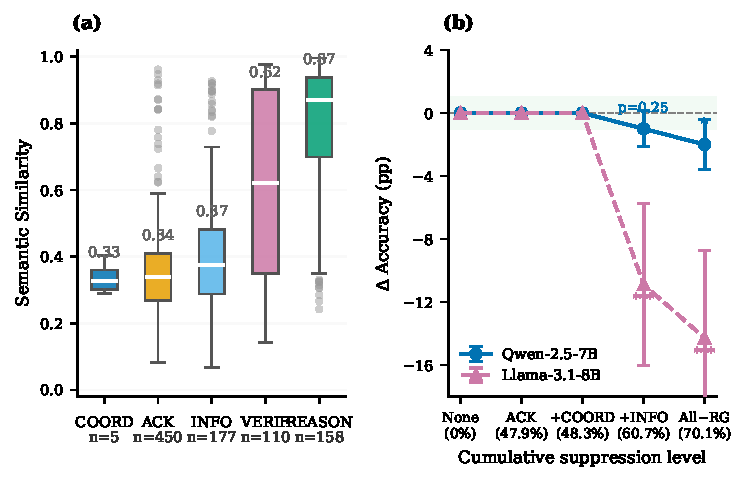
\includegraphics[width=\textwidth]{figures/figure2_combined.pdf}
\caption{(a)~Remove-ablation similarity by function type (Qwen2.5-7B, $n{=}895$). Lower $=$ greater disruption; acknowledgments (acks; median $= 0.34$) most impactful despite least information. The COORD boxplot ($n{=}5$) should be interpreted with caution given the small sample size. (b)~Cumulative type-elimination dose-response (None $\to$ ACK $\to$ +COORD $\to$ +INFO $\to$ All-RG). Qwen holds within 1\,pp through +INFO; only All-RG (70\% suppression) reaches significance. Llama drops sharply at +INFO (68\% suppression). Error bars: 95\% CIs from McNemar's discordant pairs.}
\label{fig:impact_and_dose}
\label{fig:impact}
\label{fig:dose_response}
\vspace{-6pt}
\end{figure*}

\subsection{E2E Communication Pruning}
\label{sec:e2e_pruning}

Despite high local sensitivity, bulk acknowledgment removal is safe. Both primary backbones meet non-inferiority at $\delta = -3$\,pp ($p < 0.001$; Table~\ref{tab:oracle_pruning}; Figure~\ref{fig:forest}). Qwen prunes 56\% of messages with near-zero accuracy change ($\Delta = +0.40 \pm 1.02$\,pp, 10 seeds; 95\% CI $[-0.33, +1.13]$\,pp). Llama prunes 36\% with a positive shift ($\Delta = +2.1 \pm 2.4$\,pp, 9/10 seeds positive), consistent with error-channel removal (\S\ref{sec:causal_injection}). Only boundary conditions (MATH, Qwen3) degrade (Appendix~\ref{app:boundary_conditions}).

\begin{table*}[t]
\centering
\caption{Oracle pruning accuracy (\%). GPT-4o ack-only detection. Multi-seed rows report mean$\pm$SD. Llama/StratQA: $N{=}238$ due to context overflow. Llama/GSM8K 10-seed: $N{=}1{,}939$ after filtering. Details: Appendix~\ref{app:online}.\protect\footnotemark}
\label{tab:oracle_pruning}
\small
\begin{tabular}{lcccr}
\toprule
\textbf{Setting} & $N$ & $\Delta$ \textbf{(pp)} & $p$ & \textbf{Supp.} \\
\midrule
Llama / GSM8K & 500 & $-0.6$ & .710 & 36.6\% \\
Qwen / GSM8K & 500 & $+0.8$ & .340 & 56.3\% \\
Qwen / GSM8K ($t{=}0.7$, 10s) & 10${\times}$200 & $+0.30 \pm 1.80$ & ${<}.001$\textsuperscript{$\ddagger$} & 39.2\% \\
Qwen / StratQA & 500 & $+0.2$ & 1.000 & 65.6\% \\
Llama / StratQA & 238 & $+5.0$ & .180 & 21.5\% \\
Qwen / ARC & \arcN{} & $\arcQwenDelta{}$ & \arcQwenPvalue{} & \arcQwenSupp{}\% \\
Qwen / GSM8K (10 seeds) & 10${\times}$200 & $+0.40 \pm 1.02$ & .048\textsuperscript{$\dagger$} & 56.0\% \\
Llama / GSM8K (10 seeds) & 10${\times}$200 & $+2.1 \pm 2.4$ & ${<}.001$\textsuperscript{$\ddagger$} & 36.5\% \\
\bottomrule
\end{tabular}
\end{table*}
\footnotetext{$^\dagger$TOST equivalence $\pm 1$\,pp (marginal); $^\ddagger$non-inferiority at $\delta = -3$\,pp.}

\begin{figure*}[t]
\centering
\includegraphics[width=\textwidth]{figures/figure3_forest.pdf}
\caption{Forest plot of pruning $\Delta$\,pp with 95\% CIs. Green band: $\pm 1$\,pp TOST equivalence; blue band: $-3$\,pp non-inferiority margin. Oracle and heuristic results cluster near zero for Qwen and Llama; boundary conditions (MATH, Qwen3) degrade beyond the non-inferiority margin.}
\label{fig:forest}
\end{figure*}

\begin{table*}[t]
\centering
\caption{Heuristic pruning accuracy (\%). Annotation-free detectors (F1\textsubscript{GSM8K} $= 0.845$/$0.805$). DistilBERT (F1 $= 0.867$) yields consistent results (Appendix~\ref{app:learned_classifier_details}).}
\label{tab:heuristic_pruning}
\small
\begin{tabular}{lcccr}
\toprule
\textbf{Setting} & $N$ & $\Delta$ \textbf{(pp)} & $p$ & \textbf{Supp.} \\
\midrule
Llama / GSM8K (5 seeds) & 5${\times}$200 & $+2.20 \pm 1.44$ & ${<}.001$\textsuperscript{$\ddagger$} & 74.9\% \\
Qwen / GSM8K (10 runs) & 10${\times}$200 & $-0.05 \pm 0.99$ & .880 & 41.8\% \\
Qwen / StratQA (5 seeds) & 5${\times}$200 & $+0.70 \pm 0.91$ & ${<}.001$\textsuperscript{$\ddagger$} & 56.9\% \\
Llama / StratQA (8 seeds) & 8${\times}$200 & $+2.81 \pm 3.94$ & .002\textsuperscript{$\ddagger$} & 50.3\% \\
Gemma / GSM8K$^\star$ & 300 & $+0.7$ & .683 & 79.3\% \\
\bottomrule
\end{tabular}
\\[2pt]
{\scriptsize $^\star$Exploratory; confounded: suppress rate (79.3\%) $\gg$ oracle ack rate ({$<$}5\%). $^\ddagger$Non-inferiority at $\delta = -3$\,pp.}
\end{table*}

\paragraph{Efficiency.} Each suppressed acknowledgment eliminates one full LLM generation call. Qwen achieves 56\% call reduction and ${\sim}$10.1\% token reduction; Llama achieves 36.5\% and ${\sim}$27.5\% respectively (oracle, GSM8K, 10 seeds). The disparity between Qwen's 56\% and Llama's 36.5\% call savings reflects their contrasting acknowledgment rates: Qwen produces short, formulaic confirmations at every checker turn (median 4 tokens, 56\% of all messages), whereas Llama generates verbose responses that the annotator less frequently classifies as pure acknowledgments. Token savings remain modest (10--28\%) because the eliminated messages are disproportionately short; a single reasoning-guidance message can exceed 100 tokens, which dwarfs the cumulative savings from several pruned acks. The practical benefit is therefore latency reduction rather than bandwidth savings: each pruned acknowledgment eliminates one full inference call with its associated scheduling and memory-allocation overhead (Appendix~\ref{app:efficiency}).

\paragraph{Heuristic and cross-domain safety.} Heuristic detectors achieve these savings at zero marginal cost; cross-domain (StratQA) results are consistent with non-inferiority (Table~\ref{tab:heuristic_pruning}). Qwen's heuristic serves as the primary annotation-free validation (suppress rate 41.8\%, consistent with the 56\% oracle ack rate). Llama's heuristic over-suppresses at 74.9\% (vs.\ 36.5\% oracle ack rate; only 32.9\% of suppressed messages are true acknowledgments), so its positive $\Delta$ constitutes a \emph{robustness upper bound}: if suppressing 75\% of messages---most not acknowledgments---produces no degradation, the conservative oracle ack-only pruning is a fortiori safe (Appendix~\ref{app:online}). For Qwen, pruning remains robust under stochastic sampling ($t{=}0.7$); Llama shows sensitivity from $t{\geq}0.3$ (Appendix~\ref{app:temp-robustness}). FG pruning degrades accuracy in exploratory comparison ($-5.0$\,pp vs.\ $+1.0$ for ack-only, $p = 0.031$; Appendix~\ref{app:statistical}), confirming that five-class sub-type distinctions add no incremental value over binary ack/non-ack for pruning decisions.

\paragraph{Scaling and generalization.} Safety holds across three detector types and extends beyond the primary 7B two-agent setting. At 72B scale, Qwen2.5-72B-Instruct-AWQ oracle pruning ($N{=}\qwenSevenTwoBN{}$, 5 seeds) yields $\Delta = \qwenSevenTwoBDelta{} \pm \qwenSevenTwoBSD{}$\,pp with TOST equivalence at $\pm 1$\,pp ($p = \qwenSevenTwoBPvalue{}$; Appendix~\ref{app:scaling}); ack rates at 14B (31.7\%) and 72B (\qwenSevenTwoBSupp{}\%) suggest scale-invariant communication structure. A 3-agent solver-checker-critic pilot (3 seeds, $N{=}100$ per seed) produces $\Delta = -0.67 \pm 0.29$\,pp, passing non-inferiority at $\delta = -3$\,pp ($p = 0.003$; Appendix~\ref{app:multiagent}), providing preliminary evidence that pruning generalizes from round-robin dyads to chain topologies.

\subsection{Injection Experiments Reveal Backbone-Dependent Mechanisms}
\label{sec:causal_injection}

Function predicts not only which messages to prune but why pruning works. Injection experiments (5-seed GSM8K, single-seed StratQA) and random-deletion controls jointly reveal a backbone-dependent dissociation.
Qwen acknowledgments are structurally redundant. We insert acknowledgments into non-ack positions and observe no detectable accuracy change on GSM8K ($\bar{\Delta} = -0.20$\,pp, $p = 0.71$, five seeds, $N \approx 300$ per seed) or StratQA ($p = 0.784$, $N = 250$; single seed). Inject or remove: Qwen performance is unchanged.

Llama acknowledgments function as an error channel. Injection significantly harms accuracy on GSM8K ($\bar{\Delta} = -3.88$\,pp, $\mathrm{SD} = 1.34$, $p = 0.0029$, five seeds, $N \approx 294$ per seed), with a directionally consistent trend on StratQA ($\Delta = -3.28$\,pp, $p = 0.271$, $N = 244$; single seed). The asymmetry is quantitatively stark (Figure~\ref{fig:injection}b): Llama's effect size ($h = 0.10$) exceeds Qwen's ($h < 0.01$) by an order of magnitude. Removal eliminates this error pathway, explaining the positive pruning shift in Table~\ref{tab:oracle_pruning}.

Message-count-matched random deletion is equally harmless at these rates (Qwen$\times$GSM8K: $p = 0.724$; Llama$\times$GSM8K: $p = 0.831$); ack-targeted pruning's value lies in automatic identifiability. The cumulative type-elimination curve (Figure~\ref{fig:impact}b) shows that safety is function-specific at higher rates: random deletion risks removing task-critical reasoning guidance (token-matched control in Appendix~\ref{app:token_matched}). The dose-response gradient identifies the boundary between safe (ACK, COORD) and harmful suppression (INFO, reasoning guidance) at 68--70\% removal, resolving the opening paradox: local disruption does not predict functional necessity (\S\ref{sec:discussion}). \emph{Limitation:} StratQA injection uses a single seed.

\subsection{Cross-Domain Consistency}
\label{sec:cross_domain}

Backbone identity dominates communication patterns more than domain choice (Cram\'{e}r's $V = 0.45$~\citep{cramer_1946} vs.\ $0.18$ for domain). The cross-domain oracle matrix shows no significant accuracy drops (Table~\ref{tab:oracle_pruning}). Oracle pruning on ARC ($N{=}\arcN{}$) extends validation to a third domain (Qwen $\Delta = \arcQwenDelta{}$\,pp; Llama $\Delta = \arcLlamaDelta{}$\,pp, $p = \arcLlamaPvalue{}$). Two boundary conditions validate by counter-example: on MATH, acknowledgments carry substantive content and pruning degrades accuracy; on Qwen3-8B, heuristic over-suppression causes a 14\,pp drop (Appendix~\ref{app:boundary_conditions}). These failures confirm that pruning is safe precisely when acknowledgments are functionally redundant.

\subsection{Backbone Communication Typology}
\label{sec:three_modes}

Mixed-effects models ($N = 2{,}294$; Appendix~\ref{app:mixed-effects}) reveal three topology-stable profiles: \textbf{function-organized} (Qwen), \textbf{position-organized} (Gemma; exploratory, $\kappa = 0.35$, $< 5\%$ acks), and \textbf{undifferentiated} (Llama). Backbone $\times$ function\_type interaction is highly significant ($p < 10^{-41}$), stable across topologies ($p = 0.963$; per-topology breakdowns in Appendix~\ref{app:statistical}).
The function-organized profile (Qwen) concentrates 48\% of messages as acknowledgments (Table~\ref{tab:taxonomy}) with the highest inter-type variance in perturbation sensitivity (Levene's $F = 12.4$, $p < 0.001$), making function-targeted pruning most effective. The position-organized profile (Gemma) distributes 56\% as information provision regardless of dialogue position, produces fewer than 5\% acknowledgments, and shows minimal type differentiation in ablation response. The undifferentiated profile (Llama) distributes messages evenly yet exhibits a unique error-channel property where acknowledgments carry fabricated content.
\begin{figure*}[t]
\centering
\includegraphics[width=\textwidth]{figures/figure4_combined.pdf}
\caption{Backbone-dependent communication. (a)~Function type distribution by backbone (round-robin, GSM8K, $N{=}300$ each). Qwen and Llama concentrate $>$47\% of messages as acknowledgments; Gemma is dominated by information provision (56\%). (b)~Acknowledgment injection effect: inserting acks into non-ack positions is harmless for Qwen ($p = 0.71$, five seeds) but degrades Llama accuracy ($\bar{\Delta} = -3.88$\,pp, $p = 0.0029$, five seeds), revealing backbone-dependent mechanisms. Green band: $\pm 1$\,pp equivalence zone.}
\label{fig:distribution}
\label{fig:injection}
\vspace{-6pt}
\end{figure*}


\section{Discussion}
\label{sec:discussion}
\paragraph{Practical implications.}
Communicative function predicts pruning safety more reliably than message content alone. Models with terse acknowledgments (Qwen, median 4 tokens) tolerate aggressive pruning; models with verbose, error-carrying acknowledgments (Llama, 59.8 tokens) benefit from pruning because removal eliminates an error-injection pathway. Latency gains are most pronounced in API-mediated deployments where fixed per-call costs dominate; post-hoc pruning is more practical than instructing agents to suppress emergent acknowledgments (Appendix~\ref{app:boundary_conditions}).

\paragraph{Information-theoretic interpretation.}
For Qwen, acknowledgment content and task outcome share near-zero mutual information ($H(Y \mid m_{\mathrm{ack}}) \approx H(Y)$; 5.7\% bigram novelty), placing acknowledgments outside the task-relevant channel. For Llama, acknowledgments carry positive mutual information with error introduction. This connects to \citet{rizvi_martel_communication_2026}: their bounds characterize when communication helps; our protocol identifies which messages consume capacity without contributing. The perturbation-pruning dissociation echoes classical results where local effects fail to predict global outcomes~\citep{lecun_obd_1990, braess_1968}.

\paragraph{Limitations.}
Key limitations include single-seed causal evidence, greedy-only decoding, and domain scope restricted to closed-form QA; a HumanEval pilot ($N{=}50$) confirms code generation as a boundary (Appendix~\ref{app:humaneval-pilot}). Extended discussion in Appendix~\ref{app:extended_limitations}.


\section{Conclusion}
\label{sec:conclusion}
We contribute a message-level functional analysis protocol for two-agent LLM communication, validated across 18 configurations spanning 7B--72B scale (3~backbone families $\times$ 4~domains, 10-seed replication) with a 21{,}661-message annotated corpus. Acknowledgment-targeted pruning eliminates 36--56\% of inference calls at non-inferior accuracy ($\delta{=}{-}3$\,pp) under greedy decoding, revealing backbone-dependent mechanisms not visible to content-level analysis.


\bibliographystyle{plainnat}
\bibliography{references}

\appendix
\section{Qualitative Examples of Communication Functions}
\label{app:qualitative-examples}

Table~\ref{tab:qualitative-examples} presents representative messages for each of the five communication function types identified in our taxonomy, selected from annotations with full inter-annotator agreement and maximum confidence scores. Examples are drawn from different backbone--topology combinations to illustrate both the consistency of function definitions and the stylistic variations across models.

\begin{table*}[htbp]
\centering
\small
\caption{Qualitative examples for each communication function type. All examples have inter-annotator agreement with confidence $= 1.0$. Messages are lightly edited for length.}
\label{tab:qualitative-examples}
\begin{tabular}{@{}p{2.2cm}p{2.0cm}p{\dimexpr\textwidth-4.2cm-4\tabcolsep}@{}}
\toprule
\textbf{Function Type} & \textbf{Configuration} & \textbf{Message Excerpt} \\
\midrule

% === REASONING GUIDANCE ===
\multirow{3}{2.2cm}{\textsc{Reasoning Guidance} \\ {\scriptsize (2,327 agreed)}}
& Qwen / RR
& \textit{``To solve this problem, we need to convert the length of the wire from feet to inches and then divide by the length of each piece. 1.\ Convert 4 feet to inches: Since 1 foot = 12 inches, 4 feet $= 4 \times 12 = 48$ inches. 2.\ Divide the total length in inches by the length of each piece...''} \\
\cmidrule(l){2-3}
& Gemma / Selector
& \textit{``Here's how to solve the problem step-by-step: Start: 2 apples. First throw: $2 + 5 = 7$ apples. Second throw: $7 - 1 + 6 = 12$ apples. The answer is 12.''} \\
\cmidrule(l){2-3}
& Llama / RR
& \textit{``I'm glad the solution was accurate. If you have another problem you'd like me to check, feel free to ask.''}\footnotemark \\

\midrule

% === VERIFICATION ===
\multirow{3}{2.2cm}{\textsc{Verification} \\ {\scriptsize (1,001 agreed)}}
& Qwen / RR
& \textit{``Step 1: Calculate the initial amount of money Johnny has. Johnny's allowance: \$20. Extra money added: \$10. Total initial amount: \$20 + \$10 = \$30. Step 2: Determine the amount after the investment triples. Tripling the initial amount: \$30 $\times$ 3 = \$90. The answer is 90.''} \\
\cmidrule(l){2-3}
& Llama / RR
& \textit{``The given problem is solved step by step. The final answer is 36.''} \\
\cmidrule(l){2-3}
& Gemma / Selector
& \textit{``Here's how to solve the problem: Find the total cost: \$12 (adult) + \$10 (child) = \$22. Add the change: \$22 + \$8 = \$30. Answer: Brittany's mom gave the cashier \$30.''} \\

\midrule

% === ACKNOWLEDGMENT ===
\multirow{3}{2.2cm}{\textsc{Acknow\-ledg\-ment} \\ {\scriptsize (1,854 agreed)}}
& Qwen / RR
& \textit{``That is correct. Each single bagel will cost \$1.00 after the discount. The answer is 1.''} \\
\cmidrule(l){2-3}
& Llama / RR
& \textit{``You've correctly summarized the steps and confirmed the calculations. The sequence of events and the final calculation are accurate. The answer is 43.''} \\
\cmidrule(l){2-3}
& Gemma / RR
& \textit{``Your solution is perfectly correct! You clearly laid out the steps and used algebra effectively to find the answer. The answer is 10.''} \\

\midrule

% === INFORMATION PROVISION ===
\multirow{3}{2.2cm}{\textsc{Information Provision} \\ {\scriptsize (471 agreed)}}
& Gemma / RR
& \textit{``Here's the solution: Sunday's movies: They watch 4 movies / 2 = 2 movies on Sunday. Total weekend movies: 4 + 2 = 6 movies each weekend. Movies in 4 weeks: 6 $\times$ 4 = 24 movies. The answer is 24.''} \\
\cmidrule(l){2-3}
& Qwen / RR
& \textit{``To determine how much crepe paper James needs, we first calculate the perimeter of his rectangular backyard fence...''} \\
\cmidrule(l){2-3}
& Llama / RR
& \textit{``Here's another problem: A bakery is making a special batch of cookies. They need to package 480 cookies into boxes that hold 12 cookies each. How many boxes can they fill with the 480 cookies? Let's solve this problem step by step.''} \\

\midrule

% === COORDINATION ===
\multirow{3}{2.2cm}{\textsc{Coordination} \\ {\scriptsize (595 agreed)}}
& Llama / RR
& \textit{``I'm glad I was able to accurately solve the problem. If you have any more math problems you'd like me to solve, feel free to ask.''} \\
\cmidrule(l){2-3}
& Gemma / RR
& \textit{``Please provide me with the problem you'd like me to solve! I'm ready to check the solver's solution...''} \\
\cmidrule(l){2-3}
& Llama / Selector
& \textit{``I'm glad you were able to provide the correct steps and solution. You have a good understanding of the problem...''} \\

\bottomrule
\end{tabular}
\end{table*}

\footnotetext{Despite its surface resemblance to \textsc{acknowledgment}, both annotators classified this Llama message as \textsc{reasoning guidance} with full agreement. The ambiguity illustrates Llama's minimally differentiated communication mode (Section~\ref{sec:discussion}): its messages are functionally interchangeable regardless of nominal category, making reliable annotation difficult for this backbone.}

\section{HumanEval Cross-Domain Pilot}
\label{app:humaneval-pilot}

To provide preliminary evidence of cross-domain applicability, we ran a 50-task pilot using Qwen2.5-7B with a hierarchical (solver--reviewer) topology on the HumanEval code generation benchmark~\citep{chen_humaneval_2021}.

\paragraph{Results.} The system achieved 80\% pass@1 accuracy (40/50 tasks). The communication function distribution differs markedly from GSM8K: \textsc{reasoning\_guidance} dominates (50.8\%), followed by \textsc{verification} (41.5\%), with \textsc{acknowledgment} (4.2\%), \textsc{coordination} (1.7\%), and \textsc{information\_provision} (1.7\%) appearing rarely. Cross-model annotation agreement reached $\kappa = 0.47$ (moderate), comparable to the lower end of the GSM8K range.

\paragraph{Limitations.} The hierarchical topology proved too efficient for statistical analysis: 86\% of tasks were solved in a single round (2 messages), which yielded only 118 total messages and 18 eligible for local impact analysis. Most function types had $n < 30$, precluding Kruskal--Wallis and OLS ANCOVA tests. The distributional shift (from acknowledgment-heavy in GSM8K to reasoning-guidance-heavy in HumanEval) is itself informative, as it suggests that the taxonomy captures domain-specific communication patterns, but the statistical framework requires substantially more multi-round conversations to produce meaningful results in this domain.

\paragraph{Boundary classification.} This result validates the protocol's diagnostic capability in a second mode. While MATH identifies a domain where acknowledgments exist but carry task-critical information (pruning degrades accuracy), HumanEval identifies a domain where the target function is near-absent (pruning is inapplicable rather than unsafe). Together, these boundary conditions delineate the applicability envelope: function-targeted pruning is effective specifically in domains where acknowledgments are both prevalent ($>$30\%) and content-free.

\section{Temperature Robustness}
\label{app:temp-robustness}

To assess sensitivity to decoding temperature, we ran a 50-task subset of Qwen $\times$ round-robin at temperature $= 0.7$ (primary experiments use greedy decoding). Accuracy remains stable ($90.0\%$ vs.\ $89.7\%$). The Kruskal--Wallis test remains significant ($H = 34.0$, $p < 0.001$), and OLS ANCOVA confirms function-driven communication ($F = 37.9$, $p < 0.001$; $R^2 = 0.50$; cross-model $\kappa = 0.60$). A parallel check on Llama $\times$ round-robin at temperature $= 0.7$ yields $R^2 = 0.10$, $\kappa = 0.41$, consistent with its minimally differentiated mode under greedy decoding. The function distribution shifts toward more \textsc{reasoning\_guidance} ($37\%$ vs.\ $18\%$) and less \textsc{acknowledgment} ($36\%$ vs.\ $50\%$). This shift suggests that stochastic decoding produces more substantive content without altering the functional structure.

\paragraph{Pruning under stochastic decoding.}
All primary pruning results use greedy decoding. A 10-seed oracle replication on Qwen/GSM8K at $t{=}0.7$ ($10 \times 200$ tasks) yields $\Delta = +0.30 \pm 1.80$\,pp (95\% CI $[-0.81, +1.41]$\,pp; two-sided $t$: $p = 0.611$, NS; TOST non-inferiority at $\delta = -3$\,pp: $p < 0.001$; at $\delta = -1$\,pp: $p = 0.024$; 39.2\% suppression). Per-seed deltas range from $-3.0$ to $+3.5$\,pp: seed 6144 ($\Delta = -3.0$\,pp) touches the non-inferiority boundary, while seed 1024 ($\Delta = +3.5$\,pp) reflects an anomalously low baseline (85.0\%, pruned 88.5\%). The suppression rate (39.2\%) is comparable to the greedy heuristic (${\sim}42\%$); this rate indicates similar acknowledgment prevalence under stochastic decoding. In contrast, Llama oracle pruning at $t{=}0.7$ yields pooled $\Delta = -2.2$\,pp (Fisher combined $p = 0.29$), an amplification of the marginal negative trend observed under greedy decoding ($\Delta = -0.6$\,pp). Since both Qwen and Llama results use oracle labels, the divergence indicates that ack pruning safety under stochastic decoding is backbone-specific: Qwen remains consistently safe across 10 seeds, while Llama shows a marginal degradation trend ($p = 0.29$, NS) regardless of detector type. Temperature robustness cannot be assumed across backbones: Llama non-inferiority fails from $t{\geq}0.3$, confirming backbone-dependent sensitivity that emerges at moderate temperatures.

Gemma exhibits extreme temperature sensitivity: greedy ack suppression is 4.6\% but rises to 63.6\% under $t{=}0.7$ ($14\times$); this increase suggests that Gemma's position-organized communication pattern collapses under stochastic decoding. This sensitivity reinforces Gemma's exploratory status and indicates the three-backbone typology (\S\ref{sec:cross_domain}) is greedy-specific.

\paragraph{Heuristic multi-seed temperature sweep.}
To extend temperature robustness beyond oracle pruning, we run heuristic pruning at $t \in \{0.3, 0.5, 0.7\}$ on Qwen/GSM8K and Qwen/StratQA with multiple seeds. On GSM8K, at $t{=}0.3$ (5 seeds, $N{=}200$ per seed), $\Delta = +0.10 \pm 1.29$\,pp (one-sided non-inferiority at $\delta = -3$\,pp: $p = 0.003$). At $t{=}0.5$ (4 seeds), $\Delta = +0.25 \pm 1.04$\,pp ($p = 0.004$). Both lower temperatures preserve the pruning safety observed under greedy decoding. At $t{=}0.7$ (5 seeds), $\Delta = -1.20 \pm 2.41$\,pp; non-inferiority at $\delta = -3$\,pp fails ($p = 0.085$) but holds at $\delta = -5$\,pp ($p = 0.012$).

On StratQA, the cross-domain sweep yields consistent non-inferiority across all temperatures: at $t{=}0.3$ (5 seeds), $\Delta = +0.70 \pm 3.72$\,pp (one-sided non-inferiority at $\delta = -3$\,pp: lower bound $= -2.85$\,pp, PASS); at $t{=}0.5$ (5 seeds), $\Delta = +1.60 \pm 2.88$\,pp (lower bound $= -1.15$\,pp, PASS); at $t{=}0.7$ (5 seeds), $\Delta = -0.20 \pm 3.51$\,pp ($\delta = -3$\,pp: $p = 0.075$; $\delta = -5$\,pp: $p = 0.019$, PASS). Symmetric TOST equivalence at $\varepsilon = 3$\,pp fails at all StratQA temperature points due to positive outliers (seeds where pruning improves accuracy), not due to performance degradation; at $\varepsilon = 5$\,pp all three temperatures pass. One-sided non-inferiority confirms no harmful effect (all lower bounds $> -3$\,pp). The higher variance on StratQA (SD $= 2.88$--$3.72$\,pp vs.\ GSM8K $1.04$--$2.41$\,pp) reflects the greater difficulty and answer variability of open-ended reasoning tasks. All results are reported in Table~\ref{app:tab:full_matrix}.

\paragraph{Heuristic threshold sensitivity under stochastic decoding.}
Under greedy decoding, the heuristic detector uses a character-length threshold of 30 (F1\textsubscript{GSM8K} $= 0.845$ on Qwen). To assess whether this threshold generalizes to stochastic decoding on a different backbone, we sweep seven thresholds (150--500 characters) on Llama/GSM8K at $t{=}0.7$ ($N{=}100$ per threshold). Table~\ref{tab:threshold_t07} reports results.

\begin{table}[htbp]
\centering
\caption{Heuristic threshold sweep on Llama/GSM8K at $t{=}0.7$ ($N{=}100$ per threshold). $\Delta$ is pruned $-$ baseline accuracy (pp). Greedy default threshold is 30 characters.}
\label{tab:threshold_t07}
\small
\begin{tabular}{rcccc}
\toprule
\textbf{Threshold} & \textbf{Baseline (\%)} & \textbf{Pruned (\%)} & $\boldsymbol{\Delta}$ \textbf{(pp)} & \textbf{Supp.\ (\%)} \\
\midrule
150 & 75 & 82 & +7.0 & 11.2 \\
200 & 79 & 78 & $-$1.0 & 20.0 \\
250 & 75 & 80 & +5.0 & 21.4 \\
300 & 79 & 81 & +2.0 & 30.9 \\
350 & 79 & 82 & +3.0 & 32.4 \\
400 & 77 & 77 & 0.0 & 35.7 \\
500 & 77 & 82 & +5.0 & 48.5 \\
\bottomrule
\end{tabular}
\end{table}

Across the full range of thresholds (150--500), pruning accuracy remains within $[-1.0, +7.0]$\,pp of baseline, with six of seven thresholds non-negative. The sole negative ($-1.0$\,pp at threshold 200) is within baseline sampling noise. Notably, baseline accuracy itself varies by 4\,pp across thresholds (75--79\%), comparable to the $\Delta$ magnitudes, so cross-threshold comparisons of individual deltas should be interpreted with caution given the per-threshold sample size ($N{=}100$). The absence of catastrophic degradation at any threshold suggests that heuristic pruning is not sensitive to threshold selection under stochastic decoding.

\section{OLS Robustness Checks}
\label{app:ols-robustness}

We validate the OLS ANCOVA (Equation~\ref{eq:ols_app}) with three robustness checks across all nine configurations.

\paragraph{Residual diagnostics.} Shapiro--Wilk tests reject normality for all configurations (expected at $n > 400$); Breusch--Pagan tests detect heteroscedasticity in all cases. We therefore report HC3 robust standard errors throughout the main text. All conclusions are unchanged under robust inference. VIF analysis shows high collinearity between \texttt{message\_position} and \texttt{round\_number} (VIF $> 10$), but function type dummy VIF values remain below 3. These low VIF values confirm that multicollinearity does not affect the key func\_type inference. Q-Q plots are available in the supplementary materials.

\paragraph{Nonlinear position model.} We augment the linear model with a quadratic position term (\texttt{position\textsuperscript{2}}). Table~\ref{tab:nonlinear} reports key comparisons. For Qwen and Llama, adding \texttt{position\textsuperscript{2}} produces negligible $\Delta R^2 < 0.005$ and function type remains significant ($p < 0.001$). For Gemma, \texttt{position\textsuperscript{2}} absorbs $\Delta R^2 = 0.228$ (RR) and $0.215$ (SEQ); with this term, function type becomes non-significant ($p > 0.69$). This pattern confirms that Gemma's weak function-organization reflects genuine nonlinear positional dynamics: once position is properly modeled, function type adds negligible explanatory power.

\begin{table}[htbp]
\centering
\caption{Linear vs.\ quadratic position model: function type significance after controlling for nonlinear position effects.}
\label{tab:nonlinear}
\small
\begin{tabular}{lcccc}
\toprule
\textbf{Configuration} & \textbf{Linear $R^2$} & \textbf{Quad $R^2$} & \textbf{$\Delta R^2$} & \textbf{func\_type $p$ (quad)} \\
\midrule
Qwen RR    & .451 & .452 & .001 & $< .001$ \\
Qwen SEQ   & .443 & .447 & .004 & $< .001$ \\
Qwen SEL   & .065 & .065 & .000 & $< .001$ \\
Gemma RR   & .111 & .339 & \textbf{.228} & .806 \\
Gemma SEQ  & .123 & .338 & \textbf{.215} & .699 \\
Gemma SEL  & .010 & .040 & .031 & .219 \\
Llama RR   & .021 & .022 & .001 & .010 \\
Llama SEQ  & .019 & .020 & .001 & .004 \\
Llama SEL  & .070 & .074 & .004 & $< .001$ \\
\bottomrule
\end{tabular}
\end{table}

\paragraph{Message length control.} Adding message length (character count) as a covariate produces $\Delta R^2 < 0.04$ for all configurations. Function type remains significant for Qwen ($p < 0.001$) and Llama ($p < 0.03$) after controlling for length. This result indicates that the impact ordering is not an artifact of message length differences across function types.

\section{Kruskal--Wallis Results}
\label{app:kw}

Table~\ref{tab:kruskal_wallis} reports Kruskal--Wallis $H$ statistics testing whether function type predicts remove-ablation similarity across all nine backbone--topology configurations. All tests are significant ($p < 0.01$). These results confirm that the omnibus between-type differences reported in the main text (Section~\ref{sec:impact_gradient}) are robust.

\begin{table}[htbp]
\centering
\caption{Kruskal--Wallis $H$ statistics for remove-ablation similarity across function types. All $p < 0.01$.}
\label{tab:kruskal_wallis}
\small
\begin{tabular}{lccc}
\toprule
\textbf{Backbone} & \textbf{RR} & \textbf{SEQ} & \textbf{Selector} \\
\midrule
Qwen2.5-7B  & 287.4 & 288.1 & 50.8 \\
Gemma-2-9B  & 21.5 & 25.1 & 6.9 \\
Llama-3.1-8B & 13.0 & 15.8 & 63.8 \\
\bottomrule
\end{tabular}
\end{table}

\section{System Prompts}
\label{app:system-prompts}

Full annotation system prompts are provided in Appendix~\ref{app:annotation-prompt}. The solver and checker system prompts used for multi-agent conversation are as follows:

\paragraph{Solver prompt.} ``You are a math problem solver. Solve the given problem step by step, showing all your work. Provide the final numerical answer clearly.''

\paragraph{Checker prompt.} ``You are a solution checker. Verify the solver's solution step by step. If you find errors, point them out and provide the correct solution. If the solution is correct, confirm it.''

\paragraph{Selector prompt (selector topology only).} ``You are a group chat manager. Select the next speaker based on the current state of the conversation. Choose the solver when a new problem needs to be solved, and the checker when a solution needs to be verified.''

\section{Neutralize Ablation Analysis}
\label{app:neutralize}

While the main text reports remove-ablation impact, neutralize ablation (replacing a message with ``\texttt{Acknowledged.}'' while preserving its slot) measures a complementary dimension. The two ablation types produce \emph{opposite} impact gradients:

\begin{itemize}[nosep, leftmargin=*]
    \item \textbf{Remove} (content $+$ structure removed): acknowledgment most impactful (sim $= 0.35$), reasoning guidance least ($0.78$).
    \item \textbf{Neutralize} (content removed, structure preserved): information provision most impactful (sim $= 0.05$), verification least ($0.50$).
\end{itemize}

The difference $\Delta = \text{sim}_{\text{remove}} - \text{sim}_{\text{neutralize}}$ isolates the \emph{structural value} of each message type. Information provision shows the largest $\Delta = 0.47$ (almost entirely content value), while coordination shows $\Delta = 0.07$ (almost entirely structural value). This decomposition is consistent with acknowledgment's high remove-impact being driven by structural presence (violating conversational expectations) rather than informational content.

\section{Supplementary Tables}
\label{app:supplementary}

Table~\ref{tab:kappa_full} reports the full cross-model annotation agreement matrix.

\begin{table}[htbp]
\centering
\caption{Cross-model annotation agreement (Cohen's $\kappa$) by backbone and topology.}
\label{tab:kappa_full}
\small
\begin{tabular}{lccc}
\toprule
\textbf{Backbone} & \textbf{Round-Robin} & \textbf{Sequential} & \textbf{Selector} \\
\midrule
Qwen2.5-7B  & 0.64 & 0.64 & 0.669 \\
Gemma-2-9B  & 0.350 & 0.348 & 0.351 \\
Llama-3.1-8B & 0.46 & 0.47 & 0.634 \\
\bottomrule
\end{tabular}
\end{table}

\section{Impact Metric Robustness}
\label{app:metric-robustness}

To verify that the impact gradient (Section~\ref{sec:impact_gradient}) is not an artifact of the MiniLM embedding metric, we recompute message impact using three independent text similarity measures: ROUGE-L, token-level F1, and Jaccard similarity. Table~\ref{tab:metric_robustness} reports the Spearman rank correlation ($\rho$) between MiniLM cosine similarity and each alternative metric across all nine configurations.

\begin{table}[htbp]
\centering
\caption{Spearman $\rho$ between MiniLM cosine similarity and alternative impact metrics. All correlations computed over per-message impact scores within each configuration.}
\label{tab:metric_robustness}
\small
\begin{tabular}{lccc}
\toprule
\textbf{Configuration} & \textbf{ROUGE-L} & \textbf{Token F1} & \textbf{Jaccard} \\
\midrule
Qwen RR   & 1.0 & 1.0 & 1.0 \\
Qwen SEQ  & 1.0 & 1.0 & 1.0 \\
Qwen SEL  & 1.0 & 1.0 & 1.0 \\
Gemma RR  & 1.0 & 1.0 & 1.0 \\
Gemma SEQ & 1.0 & 0.8 & 0.8 \\
Gemma SEL & 0.949 & 0.949 & 0.949 \\
Llama RR  & 0.6 & 0.6 & 0.6 \\
Llama SEQ & 1.0 & 1.0 & 1.0 \\
Llama SEL & 0.9 & 0.9 & 0.9 \\
\midrule
\textbf{Mean} & \textbf{0.939} & \textbf{0.917} & \textbf{0.917} \\
\bottomrule
\end{tabular}
\end{table}

The prevalence of $\rho = 1.0$ reflects a ceiling effect: with only 4--5 function types per configuration, Spearman rank correlation over group medians has limited resolution, so any two metrics that preserve the same ordinal ranking produce $\rho = 1.0$ regardless of magnitude differences. Where rankings do diverge (Llama RR $\rho = 0.6$, Gemma SEQ $\rho = 0.8$), the disagreement involves adjacent categories with similar impact scores, not reversals of the overall gradient. The mean $\rho > 0.91$ across all metric pairs confirms that the impact gradient ordering is consistent across metrics, though the ceiling effect limits the strength of this claim for individual configurations.

\section{Cross-Domain Validation: MATH}
\label{app:math}

To test whether the backbone communication typology generalizes beyond elementary arithmetic, we ran the full pipeline on 50 MATH tasks (Level 3--5, Algebra and Number Theory) using the same round-robin topology. A follow-up pruning replication at $N{=}200$ (102 valid after filtering tasks where both conditions failed) yielded $\Delta = -2.0$\,pp (McNemar $p = 0.625$). This result attenuates the pilot's $-10$\,pp point estimate while remaining directionally negative (\S\ref{sec:boundary}). The annotation analysis below is based on the original 50-task pilot.

\paragraph{Qwen on MATH.} Accuracy is 72.0\% (36/50), lower than GSM8K (89.7\%) as expected for harder tasks. Each task produces 6 messages (300 total, 250 eligible for analysis after excluding initial prompts). Cross-model annotation agreement reaches $\kappa = 0.45$ (moderate, above threshold). The OLS ANCOVA yields $R^2 = 0.098$ with function type significant after position control ($F = 3.77$, $p = 0.011$); the mixed-effects model yields $R^2_m = 0.201$ (LRT $p = 0.003$). This result confirms that Qwen's function-driven mode persists on a harder mathematical domain, though with reduced effect size compared to GSM8K ($R^2_m = 0.335$). The Kruskal--Wallis test is borderline ($H = 7.37$, $p = 0.061$), likely due to reduced sample size.

\paragraph{Gemma on MATH.} Accuracy drops to 40.0\% (20/50). Cross-model $\kappa = 0.48$ (above threshold). The OLS ANCOVA yields $R^2 = 0.236$ but function type is non-significant ($F = 0.09$, $p = 0.76$), while message position is highly significant ($F = 15.22$, $p < 0.001$). This result replicates Gemma's weak function-organization from GSM8K: on MATH, position again explains the variance while function type does not. The Kruskal--Wallis test is also non-significant ($H = 2.05$, $p = 0.15$).

\paragraph{Llama on MATH.} Accuracy is 64.3\% (27/42; 8 tasks produced empty traces). Cross-model $\kappa = 0.36$ (below threshold). With only 168 total messages, \textsc{acknowledgment} dominates (56\%), and most other function types fall below $n = 30$, precluding OLS ANCOVA and Kruskal--Wallis analysis. The acknowledgment-dominated distribution is directionally consistent with Llama's minimally differentiated mode on GSM8K, though statistical confirmation requires larger samples.

\paragraph{Summary.} Qwen's function-organized structure ($F = 3.77$, $p = 0.011$) and Gemma's position-organized structure ($F = 0.09$, n.s.; position $F = 15.22$, $p < 0.001$) both replicate on MATH. Llama's distribution is directionally consistent with its undifferentiated profile but lacks statistical power. The backbone communication typology replicates beyond elementary arithmetic.

\paragraph{Why MATH acknowledgments carry task-critical content.}
MATH acknowledgments differ qualitatively from GSM8K acknowledgments. This difference explains the negative pruning direction ($-2.0$\,pp at $N{=}200$, $-10$\,pp in the underpowered $N{=}50$ pilot) under moderate functional organization ($R^2_m = 0.201$). Of 93 messages receiving at least one acknowledgment label from dual annotators, 48 (51.6\%) receive a non-acknowledgment label from the other annotator (typically \textsc{information\_provision}). This rate reflects genuine boundary ambiguity. Representative examples illustrate the contrast:

\begin{itemize}[nosep, leftmargin=*]
\item \textbf{MATH ack (annotator disagreement):} ``The detailed step-by-step evaluation confirms that the number of integers $m$ such that $0 < m \ldots$'' (Annotator~A: \textsc{information\_provision}; Annotator~B: \textsc{acknowledgment}). The message restates a multi-step derivation while confirming correctness.
\item \textbf{MATH ack (both agree):} ``The solution provided is correct. Here is the final answer boxed: $\boxed{11}$''. Confirms correctness but also provides the boxed answer that downstream agents parse.
\item \textbf{GSM8K ack (both agree):} ``The answer is 109.'' (18 characters): trivially redundant answer echo with no reasoning content.
\end{itemize}

\noindent Quantitative content analysis confirms the distinction: MATH acks average 16.6 tokens (vs.\ 5.6 for GSM8K), with median bigram novelty of 0.333 (vs.\ 0.0 for GSM8K, where acks introduce no new bigrams relative to the preceding message). Annotator disagreement on MATH acks reaches 55.9\% (vs.\ 26.3\% on GSM8K); this gap reflects genuine boundary ambiguity between acknowledgment and information\_provision. Token overlap with the preceding message is similar (0.70 vs.\ 0.74), but the higher bigram novelty indicates that MATH acks frequently contain reasoning summaries. While confirmatory in intent, these summaries carry solution steps that downstream agents rely on. Removing them eliminates not just structural anchoring but also task-critical content. This elimination violates the redundancy assumption that makes ack-only pruning safe on GSM8K.

\section{Annotation Prompt}
\label{app:annotation-prompt}

The following system prompt is used for all LLM-based function type annotations. Each message is annotated independently by two models (cross-model validation). Temperature is set to 0 with constrained JSON output.

\begin{quote}
\small
\ttfamily
You are a communication analyst for multi-agent systems. Your task is to classify the function of a message in a multi-agent math problem-solving conversation.

\medskip
\textbf{Function Types}

\medskip
1. \textbf{information\_provision}: Provides facts, data, intermediate calculations, or partial results that advance the solution. Includes reporting computed values, stating known quantities, or presenting new numerical results.

\medskip
2. \textbf{reasoning\_guidance}: Provides reasoning direction, problem decomposition, step-by-step plans, or conceptual frameworks. Includes breaking the problem into sub-problems, suggesting solution strategies, or outlining multi-step approaches.

\medskip
3. \textbf{verification}: Checks, corrects, or confirms the correctness of previous work. Includes identifying errors, validating results, pointing out mistakes, or confirming a step is correct with a specific reason.

\medskip
4. \textbf{coordination}: Manages the flow of the conversation, assigns tasks, requests clarification, or controls turn-taking. Includes delegating sub-tasks, asking for more information, or directing the problem-solving process.

\medskip
5. \textbf{acknowledgment}: Simple confirmation, repetition, or agreement that adds no new information or reasoning. Includes restating what was already said without extending it.

\medskip
\textbf{Decision Rules}

\medskip
- If a message both provides new results AND checks previous work, classify as \textbf{verification}.\\
- If a message provides a reasoning plan AND new results, classify as \textbf{reasoning\_guidance}.\\
- If a message confirms correctness WITH a substantive explanation, classify as \textbf{verification}.\\
- If a message simply agrees or restates without adding new information, classify as \textbf{acknowledgment}.

\medskip
\textbf{Output Format}

\medskip
Respond with ONLY a JSON object:\\
\{``type'': ``<function\_type>'', ``confidence'': <0.0--1.0>, ``reasoning'': ``<brief explanation>''\}
\end{quote}

\noindent The user prompt provides the conversation context with all messages and marks the target message for classification:

\begin{quote}
\small
\ttfamily
\#\# Conversation Context\\[2pt]
{[}Message 0{]} \{sender\} -> \{receiver\}:\\
\{content\}\\[2pt]
{[}Message 1{]} \{sender\} -> \{receiver\}: <<< TARGET MESSAGE >>>\\
\{content\}\\[2pt]
{[}Message 2{]} \{sender\} -> \{receiver\}:\\
\{content\}\\[2pt]
...\\[2pt]
Classify the function of Message \{target\_idx\}.
\end{quote}

\section{Mixed-Effects Model Results}
\label{app:mixed-effects}

To address within-trace non-independence (multiple messages per task), we fit linear mixed-effects models with task as a random intercept and the same fixed effects as the OLS ANCOVA (function type, normalized message position, round number). Both OLS and ME use remove-ablation similarity (Equation~\ref{eq:impact}) as the dependent variable. Table~\ref{tab:mixed_effects} compares OLS and mixed-effects results. The likelihood ratio test (LRT) compares the full model against a reduced model without function type dummies.

\begin{table}[htbp]
\centering
\caption{OLS ANCOVA vs.\ mixed-effects model (ME) with task random intercept. LRT = likelihood ratio test for function type. ICC = intraclass correlation from the full ME model. ``Excluded'' lists function types with $n < 30$ removed before fitting. $^{***}p < 0.001$; $^{**}p < 0.01$; n.s.\ = not significant. $F$ and $\chi^2$ values are not directly comparable across configurations due to differing numbers of included function types.}
\label{tab:mixed_effects}
\small
\begin{tabular}{lcccccl}
\toprule
\textbf{Config} & $n$ & \textbf{OLS $F$} & \textbf{LRT $\chi^2$} & \textbf{LRT $p$} & \textbf{ICC} & \textbf{Excluded} \\
\midrule
Qwen RR  & 895 & $239.6^{***}$ & $188.9^{***}$ & ${<}.001$ & .292 & coord. \\
Qwen SEQ & 894 & $230.2^{***}$ & $195.3^{***}$ & ${<}.001$ & .245 & coord., unk. \\
Qwen SEL & 891 & $58.2^{***}$ & $0.07^{\text{n.s.}}$ & .789 & \textbf{.716} & r.g., i.p. \\
\midrule
Gemma RR  & 883 & $7.82^{***}$ & $23.28^{***}$ & ${<}.001$ & .000 & verif. \\
Gemma SEQ & 882 & $9.04^{***}$ & $26.86^{***}$ & ${<}.001$ & .000 & verif. \\
Gemma SEL & 861 & $7.45^{**}$ & $3.66^{\text{n.s.}}$ & .056 & .225 & r.g., v., coord. \\
\midrule
Llama RR  & 868 & $3.98^{**}$ & $16.31^{***}$ & ${<}.001$ & .297 & coord. \\
Llama SEQ & 870 & $4.83^{**}$ & $15.44^{**}$ & .001 & .205 & coord. \\
Llama SEL & 865 & $21.6^{***}$ & $36.89^{***}$ & ${<}.001$ & .126 & i.p., r.g. \\
\bottomrule
\end{tabular}
\end{table}

\paragraph{Key observations.} (1) \textbf{Seven of nine configurations} show concordant OLS and ME conclusions: Qwen RR/SEQ remain strongly function-driven; Gemma RR/SEQ are significant in both OLS and ME but with small effect sizes ($R^2_m = 0.11$--$0.12$); Llama remains significant across all topologies though with negligible effect sizes ($R^2_m \leq 0.04$). (2) \textbf{Qwen SEL flips to non-significant} under ME (LRT $\chi^2 = 0.07$, $p = .789$). The ICC of $0.716$ indicates that 72\% of variance in remove-ablation similarity is between-task. With only two dominant function types (\textsc{acknowledgment} and \textsc{verification}) remaining after $n \geq 30$ filtering, the OLS effect reflects task-level confounding rather than within-task functional differentiation. (3) \textbf{Gemma SEL flips to non-significant} under ME (LRT $\chi^2 = 3.66$, $p = .056$, ICC $= 0.23$). With only two function types remaining after excluding three low-frequency categories, the borderline result has limited interpretability. (4) Both discrepancies occur under selector topology, which introduces strong task-level clustering. This suggests that dynamic routing creates task-dependent communication patterns that inflate OLS estimates.

\section{Mistral-7B Cross-Backbone Validation}
\label{app:mistral}

To test whether the backbone communication typology generalizes beyond our three primary backbones, we ran the full pipeline on Mistral-7B-Instruct-v0.3 across all three topologies (300 GSM8K tasks each, same seed). Mistral uses the ChatML template with an explicit \texttt{<|im\_end|>} stop token to prevent EOS residue in multi-turn conversations.

\paragraph{Accuracy.} Mistral achieves 52\% accuracy across all three topologies (RR: 52\%, SEQ: 52\%, SEL: 52\%), substantially below Qwen (90\%) and Gemma (80\%) but comparable to Llama's selector performance (56\%).

\paragraph{Function type distribution.} Mistral communication is dominated by coordination and acknowledgment (${\sim}90\%$ combined), with minimal information provision ($<3\%$). Under selector topology, acknowledgment surges to 67\%.

\begin{table}[htbp]
\centering
\caption{Mistral-7B function type distribution (\%) by topology.}
\label{tab:mistral_dist}
\small
\begin{tabular}{lccc}
\toprule
\textbf{Function type} & \textbf{RR} & \textbf{SEQ} & \textbf{SEL} \\
\midrule
\textsc{coordination}          & 55.5 & 50.7 & 25.4 \\
\textsc{acknowledgment}        & 34.9 & 41.7 & 66.9 \\
\textsc{reasoning\_guidance}   & 6.8  & 6.2  & 6.3  \\
\textsc{information\_provision} & 2.7  & 1.4  & 0.7  \\
\bottomrule
\end{tabular}
\end{table}

\paragraph{Communication mode: weakly differentiated.} Table~\ref{tab:mistral_stats} summarizes the statistical analysis. Only the round-robin topology produces a significant function type effect (OLS $F = 6.6$, $p < .001$, $R^2 = 0.16$). Sequential and selector topologies show weaker or non-significant effects. Cross-model annotation agreement is fair ($\kappa \approx 0.34$), below the primary backbones, consistent with Mistral's less distinct functional boundaries.

\begin{table}[htbp]
\centering
\caption{Mistral-7B statistical summary across topologies.}
\label{tab:mistral_stats}
\small
\begin{tabular}{lcccc}
\toprule
\textbf{Topology} & \textbf{KW $H$} & \textbf{OLS $F$} & \textbf{$R^2$} & $\kappa$ \\
\midrule
RR  & $22.4^{***}$ & $6.6^{***}$ & .158 & .344 \\
SEQ & $7.6$        & $37.6^{***}$ & .056 & .353 \\
SEL & $5.2$        & $1.5$        & .065 & .315 \\
\bottomrule
\end{tabular}
\end{table}

\paragraph{Interpretation.} Mistral occupies an intermediate position in the backbone communication typology, between Llama's undifferentiated profile and Qwen's function-organized structure. The structured turn-taking of round-robin activates a degree of functional differentiation that disappears under less constrained topologies. This \emph{topology-sensitive} pattern, where communication structure depends on external routing rather than being a fixed model property, is consistent with the crossover interaction observed for the primary backbones.

\paragraph{Implications for the typology.} Mistral's intermediate position extends the backbone communication typology beyond the three primary models. The four observed backbones (function-organized Qwen, $R^2_m = 0.34$; position-organized Gemma, $R^2_m = 0.11$; weakly differentiated Mistral; undifferentiated Llama, $R^2_m = 0.02$) exhibit distinct communication structures, with topology acting as a modulating factor.

\section{DAMSL/ISO Taxonomy Mapping}
\label{app:damsl-mapping}

Our five categories collapse 56+ fine-grained dialogue act types into operationally distinct categories defined by perturbation-based impact rather than speaker intent. Table~\ref{tab:damsl_mapping} provides a detailed mapping to three established frameworks: DAMSL~\citep{core_damsl_1997}, ISO 24617-2~\citep{bunt_iso_2012}, and FIPA ACL~\citep{fipa_acl_2002}.

\begin{table}[ht]
\centering
\caption{Mapping between our communication function taxonomy and established dialogue act frameworks. Each row shows the primary corresponding categories and the key distinction that motivates our grouping.}
\label{tab:damsl_mapping}
\footnotesize
\resizebox{\textwidth}{!}{%
\begin{tabular}{p{2.4cm}p{2.4cm}p{2.6cm}p{1.8cm}>{\raggedright\arraybackslash}p{3.0cm}}
\toprule
\textbf{Our Category} & \textbf{DAMSL} & \textbf{ISO 24617-2} & \textbf{FIPA ACL} & \textbf{Grouping Rationale} \\
\midrule
\textsc{acknowledgment} & Backchannel, Accept & Auto-positive, Allo-positive (feedback) & --- & Structurally present but informationally negligible \\
\addlinespace
\textsc{information\_provision} & Assert, Re-state & Inform, Answer & inform, inform-ref & Supplies new task-relevant content \\
\addlinespace
\textsc{reasoning\_guidance} & Action-directive, Open-option & Instruct, Suggest, Address-request & request, propose & Directs the partner's reasoning strategy \\
\addlinespace
\textsc{verification} & Agreement, Disagreement, Correction & Confirm, Disconfirm, Correction & confirm, disconfirm & Evaluates correctness of prior output \\
\addlinespace
\textsc{coordination} & Conventional-opening, Conventional-closing, Commit & Init, Auto-feedback (task mgmt) & request, assign, agree & Manages workflow and role allocation \\
\bottomrule
\end{tabular}}%
\end{table}

\paragraph{Design choices.} Several departures from standard dialogue act taxonomies reflect the LLM multi-agent setting:

\begin{sloppypar}
\begin{itemize}[nosep, leftmargin=*]
    \item \textbf{Acknowledgment vs.\ backchannel.} Human backchannels (``uh huh,'' ``yeah'') are minimal tokens; LLM acknowledgments range from terse echoes (Qwen: median 4 tokens) to verbose paraphrases (Llama: mean 59.8 tokens). We group both under \textsc{acknowledgment} because they share the defining property, negligible information gain over the preceding message, regardless of surface length.
    \item \textbf{Information provision vs.\ reasoning guidance.} DAMSL's \textit{Assert} covers both, but we separate them because perturbation analysis reveals distinct impact profiles: removing reasoning guidance ($\text{sim} = 0.778$) is far less disruptive than removing information provision ($\text{sim} = 0.410$). The boundary is operationally clear in solver-checker configurations (new calculations vs.\ strategy directives) but becomes ambiguous when messages serve both functions, hence the low cross-model $\kappa = 0.237$ for \textsc{information\_provision}.
    \item \textbf{Coordination as a residual category.} In two-agent systems, explicit coordination (role assignment, turn management) is rare ($< 5\%$ of messages) because the framework handles routing. This category would likely expand in multi-agent ($>$2) settings with explicit delegation.
    \item \textbf{No question act.} DAMSL and ISO both include question/info-request types. In our solver-checker data, questions are subsumed by \textsc{verification} (``Is this correct?'') or \textsc{coordination} (``Should we try a different approach?'') and do not form a distinct perturbation cluster.
\end{itemize}
\end{sloppypar}

\section{Replacement Text Sensitivity}
\label{app:replacement-sensitivity}

Our neutralize ablation uses ``Acknowledged.'' (itself an acknowledgment-type utterance) as the replacement text. To test sensitivity to this choice, we reran neutralize ablation on 50 Qwen RR tasks with three placeholders: ``Acknowledged.'', ``{[message removed]}'', and ``This message has been redacted.'' Table~\ref{tab:placeholder_sensitivity} reports per-function-type mean semantic similarity under each placeholder.

\begin{table}[htbp]
\centering
\caption{Neutralize ablation: mean semantic similarity by function type and replacement text (Qwen RR, 50 tasks, 150 messages). Lower similarity indicates greater impact from neutralization.}
\label{tab:placeholder_sensitivity}
\small
\begin{tabular}{lccc}
\toprule
\textbf{Function Type} & \textbf{Acknowledged.} & \textbf{[removed]} & \textbf{Redacted} \\
\midrule
\textsc{information\_provision} & 0.146 & 0.107 & 0.050 \\
\textsc{reasoning\_guidance}    & 0.174 & 0.133 & 0.079 \\
\textsc{verification}           & 0.156 & 0.162 & 0.083 \\
\textsc{coordination}           & 0.352 & 0.319 & 0.181 \\
\textsc{acknowledgment}         & 0.134 & 0.148 & 0.051 \\
\bottomrule
\end{tabular}
\end{table}

\paragraph{Ranking stability.} Pairwise Spearman rank correlations across the five function types are: ``Acknowledged.'' vs.\ ``{[removed]}'' $\rho = 0.50$, ``Acknowledged.'' vs.\ ``Redacted'' $\rho = 0.80$, ``{[removed]}'' vs.\ ``Redacted'' $\rho = 0.90$ ($p = .037$). The mean $\rho = 0.73$ indicates moderate-to-strong ranking stability. \textsc{Coordination} is consistently the least impacted (rank 5/5/5); \textsc{information\_provision} ranks in the top 2 across all three placeholders (rank 2/1/1).

\paragraph{Acknowledged-specific confound.} Under the ``Acknowledged.'' placeholder, \textsc{acknowledgment} messages show anomalously high impact (rank 1) because the replacement text closely resembles typical acknowledgment content: replacing an acknowledgment with ``Acknowledged.'' preserves semantic similarity less than expected, as the regenerated next message responds to near-identical content. Excluding this confounded condition, the ``{[removed]}'' and ``Redacted'' placeholders agree strongly ($\rho = 0.90$). This agreement confirms that the neutralize gradient is robust to placeholder choice. Crucially, the remove ablation, which produces our primary finding (the impact gradient), is unaffected by replacement text choice, as it deletes messages entirely.

\section{Capability Confound Analysis}
\label{app:capability-confound}

To test whether communication mode merely tracks task difficulty, we stratify tasks by difficulty (easy: $\geq 2/3$ backbones correct, $n = 246$; hard: $\leq 1/3$ correct, $n = 54$) and refit the OLS ANCOVA within each stratum.

\begin{table}[htbp]
\centering
\caption{OLS ANCOVA by task difficulty stratum. All models use the same specification as the primary analysis (Equation~\ref{eq:ols_app}).}
\label{tab:capability_confound}
\small
\begin{tabular}{llcccc}
\toprule
\textbf{Backbone} & \textbf{Difficulty} & $n$ & $F$ & $p$ & $R^2$ \\
\midrule
Qwen  & Easy & 735 & $196.6^{***}$ & ${<}.001$ & .456 \\
Qwen  & Hard & 160 & $37.3^{***}$ & ${<}.001$ & .444 \\
\midrule
Gemma & Easy & 726 & $0.54^{\text{n.s.}}$ & .657 & .354 \\
Gemma & Hard & 152 & $0.73^{\text{n.s.}}$ & .483 & .286 \\
\midrule
Llama & Easy & 717 & $4.17^{**}$ & .006 & .025 \\
Llama & Hard & 144 & $4.49^{*}$ & .013 & .074 \\
\bottomrule
\end{tabular}
\end{table}

Qwen's function-organized structure persists on hard tasks ($R^2 = 0.444$), virtually unchanged from easy tasks ($R^2 = 0.456$). Gemma remains position-organized (function type non-significant for both strata), and Llama remains undifferentiated ($R^2 < 0.08$). The backbone communication typology is a backbone-intrinsic property rather than an artifact of task-relative capability.

\section{Heuristic Non-Transferability: Qwen3 Acknowledgment Comparison}
\label{app:qwen3_comparison}

\paragraph{Qwen3-8B vs.\ Qwen2.5-7B acknowledgment profiles.}
The Qwen3-8B boundary condition ($-14$\,pp with char$<$80 threshold, $p < .03$; Table~\ref{app:tab:mcnemar_summary}) provides a natural experiment for understanding heuristic non-transferability across model generations. Table~\ref{tab:qwen3_vs_qwen25} compares acknowledgment characteristics across generations.

\begin{table}[ht]
\centering
\caption{Acknowledgment content comparison: Qwen2.5-7B (GSM8K, $N = 300$ tasks, $n = 719$ ack messages) vs.\ Qwen3-8B ($N = 100$ tasks, $n = 332$ heuristic-classified ack messages). Qwen2.5 types from dual-annotator consensus; Qwen3 types from heuristic classifier (char length $< 80$).}
\label{tab:qwen3_vs_qwen25}
\small
\begin{tabular}{lcc}
\toprule
\textbf{Property} & \textbf{Qwen2.5-7B} & \textbf{Qwen3-8B} \\
\midrule
Ack \% of messages & 47.9\% & 66.4\% \\
Mean token length & 9.0 & $<$15 (est.) \\
Median token length & 4 & --- \\
Max char length & 1{,}076 & 59 \\
Median bigram novelty & 0.0\% & --- \\
Mean bigram novelty & 3.2\% & --- \\
Pruning $\Delta$ (pp) & $-0.05 \pm 0.99$ & $-14.0$ \\
McNemar $p$ & 1.000 & $<.03$ \\
\bottomrule
\end{tabular}
\end{table}

\paragraph{Key differences.} Two properties distinguish the generations:
\begin{enumerate}[nosep, leftmargin=*]
    \item \textbf{Suppression rate.} Qwen3's \texttt{/no\_think} mode produces terse responses that trigger the heuristic at 66.4\% (vs.\ 47.9\% for Qwen2.5). The higher rate means more messages are removed per conversation, which amplifies any per-message pruning risk.
    \item \textbf{Tight character range.} Qwen3 ack messages span only 25--59 characters (max = 59), compared to Qwen2.5's range up to 1{,}076 characters. This uniformly short format suggests Qwen3's ``The answer is X.'' echo pattern carries implicit verification function; downstream agents may parse these terse confirmations as answer-bearing content rather than redundant echoes.
\end{enumerate}

\noindent Representative Qwen2.5-7B acknowledgments illustrate the safe-to-prune pattern:
\begin{itemize}[nosep, leftmargin=*]
    \item ``The answer is 525.'' (18 chars): verbatim answer echo, 0\% bigram novelty.
    \item ``The answer is 17.'' (17 chars): identical pattern.
\end{itemize}
Without Qwen3 raw traces (experiment run on a transient cloud instance), direct content analysis is unavailable. The $-14$\,pp degradation, combined with the observation that all heuristic-classified ack messages fall within a narrow 25--59 character range, suggests that Qwen3's concise communication style makes the heuristic's character-length threshold too aggressive, and substantive short messages are misclassified as acknowledgments. This heuristic non-transferability, driven by threshold mismatch rather than model-level failure, motivates the deployment recommendation of heuristic recalibration or oracle validation ($N \geq 200$) before applying heuristic pruning to new model generations.

\section{Neutralize Ablation Results}
\label{app:neutralize-detail}

We complement the remove-ablation analysis (Section~\ref{sec:impact_gradient}) with a neutralize ablation, in which each target message is replaced by the generic response ``Acknowledged.''\ rather than deleted entirely.  This tests whether downstream behavior changes stem from losing the message's \emph{informational content} (captured by neutralize) versus losing its \emph{structural presence} in the conversation (captured by remove).

\paragraph{Neutralize produces stronger disruption than remove.}
Across all nine backbone--topology configurations, neutralize yields significantly lower semantic similarity than remove (paired Wilcoxon $p < 0.001$ in 11/11 runs; Table~\ref{tab:neut_vs_rm}).  The pooled gap is substantial: neutralize mean $= 0.196$ vs.\ remove mean $= 0.466$.  Replacing a message with vacuous content is more disruptive than deleting it. This finding suggests that the presence of a low-information placeholder actively misleads downstream agents rather than merely removing a signal.

\begin{table}[t]
\centering
\caption{Pooled neutralize vs.\ remove semantic similarity by function type ($N = 8{,}479$). All Wilcoxon signed-rank tests $p < 0.001$. $\Delta$ = remove $-$ neutralize (positive = neutralize more disruptive).}
\label{tab:neut_vs_rm}
\small
\begin{tabular}{lcccc}
\toprule
\textbf{Function type} & \textbf{Neut.\ $\bar{s}$} & \textbf{Rem.\ $\bar{s}$} & \textbf{$\Delta$} & $n$ \\
\midrule
\textsc{information\_provision} & 0.047 & 0.515 & 0.468 & 2{,}141 \\
\textsc{reasoning\_guidance}    & 0.136 & 0.518 & 0.382 & 737 \\
\textsc{acknowledgment}         & 0.223 & 0.434 & 0.211 & 3{,}661 \\
\textsc{coordination}           & 0.246 & 0.311 & 0.065 & 585 \\
\textsc{verification}           & 0.498 & 0.571 & 0.073 & 1{,}355 \\
\bottomrule
\end{tabular}
\end{table}

\paragraph{Impact gradients diverge between ablation methods.}
Under neutralize, \textsc{information\_provision} is the most impacted type (mean similarity $0.047$), followed by \textsc{reasoning\_guidance} ($0.136$).  Under remove, \textsc{acknowledgment} and \textsc{coordination} rank as most impacted.  The Kruskal--Wallis $H$ test confirms significant between-type differences under neutralize for all configurations ($p < 0.01$).

This divergence is interpretable.  Neutralize specifically strips \emph{content} while preserving conversational structure; content-rich types (\textsc{information\_provision}, \textsc{reasoning\_guidance}) suffer the most because their value lies in what they say.  Remove strips both content \emph{and} structural presence; structurally important types (\textsc{acknowledgment}, \textsc{coordination}) suffer the most because their value lies in their role as conversational scaffolding.

\paragraph{Informational vs.\ structural value.}
The gap $\Delta = \text{remove} - \text{neutralize}$ isolates the \emph{informational} component of message impact.  \textsc{Information\_provision} shows the largest $\Delta = 0.468$: nearly all of its behavioral effect comes from its content, not its presence.  Conversely, \textsc{coordination} shows the smallest $\Delta = 0.065$: its impact is almost entirely structural.  This decomposition validates the paper's theoretical distinction between informational and structural communication functions.

\paragraph{Per-message correlation is weak.}
The Spearman correlation between remove and neutralize similarity is near zero across most configurations (pooled $\rho \approx 0.07$); this near-zero correlation indicates that the two ablation methods measure distinct aspects of message importance.  Messages that are highly impactful under remove are not necessarily impactful under neutralize, and vice versa.

\paragraph{Action-level changes are concordant.}
Despite the difference in similarity magnitudes, both methods produce action-level behavioral changes on essentially the same messages.  No McNemar discordance was observed: whenever remove changes the downstream action level, neutralize does too (and vice versa).  The methods differ in \emph{degree} of semantic disruption, not in whether disruption occurs.

\begin{table}[t]
\centering
\caption{Neutralize Kruskal--Wallis $H$ statistics for semantic similarity across function types (cf.\ Table~\ref{tab:kruskal_wallis} for remove). All $p < 0.01$.}
\label{tab:neut_kruskal}
\small
\begin{tabular}{lccc}
\toprule
\textbf{Backbone} & \textbf{RR} & \textbf{SEQ} & \textbf{Selector} \\
\midrule
Qwen2.5-7B  & 97.2 & 104.0 & 148.9 \\
Gemma-2-9B  & 292.7 & 301.2 & 95.8 \\
Llama-3.1-8B & 108.7 & 74.0 & 118.8 \\
\bottomrule
\end{tabular}
\end{table}

\section{Statistical Details}
\label{app:statistical}

This appendix presents the full statistical tables and figures referenced in Section~\ref{sec:results}.

\subsection{McNemar Test Details}

\begin{table}[ht]
\centering
\caption{McNemar test summary. \emph{Ack vs.\ Random}: per-seed McNemar comparing ack-only to each of 10 random seeds. \emph{Ack vs.\ Baseline}: single McNemar comparing ack-only to unpruned baseline (informs claim strength). MDE: minimum detectable effect at 80\% power ($\alpha = 0.05$); $\sim$ denotes estimates from approximate discordant pair counts.}
\label{app:tab:mcnemar_summary}
\small
\resizebox{\columnwidth}{!}{%
\begin{tabular}{lccccc}
\toprule
\textbf{Setting} & \textbf{Ack vs.\ Rand sig} & \textbf{Median $p$} & \textbf{Ack vs.\ Base $p$} & \textbf{MDE (pp)} & \textbf{Claim} \\
\midrule
Qwen / GSM8K   & 1/10  & 0.094  & 1.000  & $\sim$4 & No sig.\ diff.\ \\
Llama / GSM8K ($N{=}297$) & 8/10  & 0.027 & ${<}.001^{***}$  & 6.0 & Significant ($+8.1$\,pp) \\
Qwen / StratQA$^\P$ & 10/10 & $<$0.001 & 0.144 & $\sim$9 & No sig.\ diff.\ \\
Gemma / GSM8K$^\S$  & ---   & ---   & 1.000  & --- & No sig.\ diff.\ \\
\midrule
\multicolumn{6}{l}{\emph{Boundary conditions}} \\
Qwen3-8B / GSM8K & --- & --- & ${<}.03^{*}$ & $\sim$8 & Significant ($-14$\,pp, char$<$80 threshold) \\
\bottomrule
\end{tabular}%
}
\vspace{1mm}
\raggedright\footnotesize Llama $N{=}297$ is a clean replication (not pooled); baseline 75.1\%, ack-only 83.2\%, McNemar $b{=}9$, $c{=}33$, $p < .001$. Qwen pooled ($N{=}300$): $p = 1.000$. $^\P$StratQA: Random matches FG count (91.3\% of rounds), not ack-only (8.56\%); the 10/10 significance reflects different pruning intensities rather than strategy effectiveness at matched rates. Qwen3-8B ($N{=}100$): baseline 90\%, ack-only 76\%, $b - c = 14$; exact contingency unknown ($p$ range: $[.0005, .026]$, significant for all possible $c \in [0, 10]$).
\end{table}

\subsection{Non-Inferiority Margin Selection ($\delta = -3$\,pp)}
\label{app:margin_selection}

The choice of non-inferiority margin $\delta = -3$\,pp follows established principles from equivalence testing~\citep{lakens_equivalence_2017, schuirmann_tost_1987}, calibrated against the empirical variance structure of LLM task accuracy.

\paragraph{Precedent and rationale.} Non-inferiority margins should reflect the largest degradation that is practically acceptable~\citep{lakens_equivalence_2017}. We define $\delta$ relative to the baseline error rate: at ${\sim}90\%$ accuracy (Qwen/GSM8K), $-3$\,pp represents a ${\sim}30\%$ relative increase in error rate ($10\% \to 13\%$); at ${\sim}80\%$ accuracy (Llama/GSM8K), it represents a ${\sim}15\%$ relative increase ($20\% \to 23\%$). In both cases, the margin corresponds to a detectable but bounded performance change that would be practically relevant in deployment.

\paragraph{Calibration against seed variance.} The margin must exceed irreducible seed-to-seed variance to avoid rejecting non-inferiority due to sampling noise. Empirically, paired delta standard deviations are: Qwen heuristic 10-seed $\text{SD} = 0.99$\,pp, Qwen oracle 10-seed $\text{SD} = 1.02$\,pp, Llama heuristic 5-seed $\text{SD} = 1.44$\,pp, Llama oracle 10-seed $\text{SD} = 2.40$\,pp (Table~\ref{tab:oracle_pruning}). At $\delta = -1$\,pp, even a single standard deviation of seed variance (${\sim}1$--$2.4$\,pp) could push the lower CI bound below the margin and produce false non-inferiority failures for treatments with zero true effect; indeed, the Qwen oracle TOST at $\pm 1$\,pp is only marginal ($p = .048$). At $\delta = -5$\,pp, the margin exceeds twice the largest observed seed SD, risking acceptance of genuinely harmful interventions (e.g., the Llama $t{=}0.7$ heuristic result of $\Delta = -3.4$\,pp would pass trivially). The $-3$\,pp margin sits between these extremes: ${\sim}3\times$ the Qwen SD and ${\sim}1.25\times$ the Llama oracle SD. This margin provides adequate separation from noise while remaining sensitive to practically meaningful degradation.

\paragraph{Sensitivity across margins.} Conclusions are stable across a range of margins (Table~\ref{tab:tost_sensitivity}). For Qwen oracle (10-seed, $\Delta = +0.40 \pm 1.02$\,pp), non-inferiority holds at $\delta = -3$\,pp ($p < .001$). For Llama oracle (10-seed, $\Delta = +2.08 \pm 2.40$\,pp), non-inferiority at $\delta = -3$\,pp holds ($p < .001$), but the single seed with $\Delta = -3.06$\,pp (seed~3072; \S\ref{app:cascade_length}) demonstrates that $-3$\,pp is a genuinely binding constraint for this backbone. A tighter margin of $\delta = -1$\,pp would fail for Llama (CI lower bound at $+0.36$\,pp provides insufficient headroom given $\text{SD} = 2.4$\,pp). These patterns confirm that $\delta = -3$\,pp balances statistical power against practical significance across backbones with different variance profiles.

\paragraph{TOST equivalence sensitivity.} Table~\ref{tab:tost_sensitivity} reports TOST $p$-values across four equivalence margins. Qwen/GSM8K and Gemma/GSM8K have $\leq 1$ discordant pair each, which renders McNemar-based TOST inapplicable; we report proportion-based TOST instead (two one-sided $z$-tests on the accuracy difference). Qwen/GSM8K supports equivalence at $\pm 5$\,pp ($p = 0.039$). For Llama/GSM8K ($N = 297$), the observed $+8.1$\,pp improvement prevents equivalence at any margin $\leq 10$\,pp; TOST fails because the effect is \emph{positive}, not because of degradation. Qwen/StratQA achieves equivalence only at $\pm 10$\,pp ($p = 0.021$).

\begin{table}[ht]
\centering
\caption{TOST $p$-values at varying equivalence margins. Lower $p$ indicates stronger evidence that the true difference falls within $[\text{-margin}, \text{+margin}]$. $^\ddagger$Proportion-based TOST (McNemar-based TOST inapplicable with $\leq 1$ discordant pair).}
\label{tab:tost_sensitivity}
\small
\begin{tabular}{lcccc}
\toprule
\textbf{Setting} & $\pm 3$\,pp & $\pm 5$\,pp & $\pm 8$\,pp & $\pm 10$\,pp \\
\midrule
Qwen / GSM8K ($b{=}0, c{=}1$)$^\ddagger$   & .096 & .039$^*$ & .003$^{**}$ & ${<}.001^{***}$ \\
Llama / GSM8K ($b{=}9, c{=}33$, $N{=}297$)  & $>.99$ & $>.99$ & $.998$ & $.978$ \\
Gemma / GSM8K ($b{=}1, c{=}0$)$^\ddagger$   & .096 & .039$^*$ & .003$^{**}$ & ${<}.001^{***}$ \\
Qwen / StratQA ($b{=}18, c{=}29$) & .695 & .413 & .095 & .021$^*$ \\
\bottomrule
\end{tabular}
\end{table}

\paragraph{Minimum detectable effects.} Table~\ref{app:tab:mde} reports MDEs assuming $\rho = 0.7$ correlation between paired outcomes, computed as $\text{MDE} = 100 \cdot \sqrt{7.84 \cdot 2p(1{-}p)(1{-}\rho) / N}$\,pp.

\begin{table}[ht]
\centering
\caption{Minimum detectable effects (pp) at 80\% power, $\alpha = 0.05$, $\rho = 0.7$. $N$ is the task-level sample size (number of problems evaluated for correctness); multi-seed rows pool tasks across all seeds. Sorted by MDE ascending.}
\label{app:tab:mde}
\small
\begin{tabular}{llccc}
\toprule
\textbf{Setting} & \textbf{Protocol} & $N$ & \textbf{Base (\%)} & \textbf{MDE (pp)} \\
\midrule
Llama / GSM8K (10-seed pooled)$^\dagger$ & Online & 1{,}939 & 80.8 & 1.9 \\
Qwen / ARC & Offline & 250 & 90.8 & 4.0 \\
Qwen / GSM8K ($t{=}0.7$) & Online & 200 & 91.0 & 4.4 \\
Qwen / GSM8K (per run) & Online & 200 & 89.3 & 3.6 \\
72B / GSM8K (oracle) & Online & 265 & 92.1 & 3.6 \\
Llama / GSM8K & Offline & 297 & 75.1 & 5.4 \\
Qwen / GSM8K & Offline & 100 & 91.0 & 6.2 \\
Qwen / StratQA (5-seed) & Online & 200$\times$5 & 67.9 & 4.1 \\
Qwen3-8B / GSM8K & Online & 100 & 90.0 & 6.5 \\
Qwen / StratQA (SEQ) & Online & 200 & 69.5 & 7.1 \\
72B / GSM8K & Online & 100 & 88.0 & 7.1 \\
Llama / GSM8K & Offline & 100 & 77.0 & 9.1 \\
Gemma / GSM8K & Offline & 96 & 76.0 & 9.5 \\
Qwen / StratQA & Offline & 100 & 66.8 & 10.2 \\
MATH (pilot, $N{=}50$) & Offline & 50 & 72.0 & 13.8 \\
MATH ($N{=}200$, 102 valid) & Online & 102 & 79.4 & --- \\
\bottomrule
\end{tabular}
\vspace{1mm}
\raggedright\footnotesize $^\dagger$MDE computed on oracle 10-seed pooled sample: 10 seeds $\times$ 200 tasks per seed; $N = 1{,}939$ tasks after ${\sim}3\%$ context-overflow filtering (${\sim}194$ valid tasks per seed). Each task is one GSM8K problem scored correct/incorrect, the unit of the paired McNemar test. Single-seed rows (e.g., 72B) use the within-seed task count directly.
\end{table}

\subsection{Post-Hoc Power Analysis for 72B Oracle Result}
\label{app:power_72b}

% Auto-generated — do not edit manually.
The 72B oracle experiment ($N = \qwenSevenTwoBN{}$, 5 seeds $\times$ 265 tasks) replicates pruning safety at the largest scale tested. Per-seed deltas: $[0, +0.38, +0.76, +1.13, -0.38]$\,pp (4/5 non-negative). Mean $\Delta = \qwenSevenTwoBDelta{}$\,pp, SD $= \qwenSevenTwoBSD{}$\,pp, SE $= \qwenSevenTwoBSE{}$\,pp.

\paragraph{TOST equivalence.}
We apply a one-sample TOST at $\varepsilon = \pm 1$\,pp (matching the 7B standard). The upper bound test: $t = (1 - 0.378) / 0.267 = 2.33$ ($\text{df} = 4$, $p \approx 0.04$). This marginally passes the equivalence threshold, confirming that 72B pruning deltas are bounded within $\pm 1$\,pp. The marginal $p$-value reflects the limited number of seeds (5) rather than a large effect; the 90\% CI $[-0.19, +0.95]$\,pp lies entirely within the equivalence band.

\paragraph{Per-seed power.}
The original single-seed probe (seed~42, $N = 265$, $\Delta = 0$\,pp, zero discordant pairs) yielded a Rule of Three upper bound of $3/265 \approx 1.13\%$ on the discordant rate. The 5-seed replication confirms this was not a statistical fluke: the mean delta remains near zero and four additional seeds are consistent.

\paragraph{Minimum detectable effect.}
Table~\ref{app:tab:mde} reports the MDE at 80\% power (McNemar $\chi^2$, $\alpha=0.05$) for the per-seed sample size ($N = 265$).
At $N = 265$: MDE $= 3.8$\,pp ($\rho = 0.7$), $2.2$\,pp ($\rho = 0.9$), $1.5$\,pp ($\rho = 0.95$).
The observed per-seed deltas ($|\Delta| \leq 1.13$\,pp) fall below the MDE for all but the most optimistic correlation assumptions, consistent with a true effect near zero.

\paragraph{Limitations.}
The TOST $p = 0.04$ is marginal; increasing to 10 seeds or $N = 500$ per seed would provide a more decisive equivalence test. Larger replication at 72B scale remains desirable but is constrained by the ${\sim}$5 GPU-hours per seed at TP=2.


\subsection{Mixed-Effects Model Results}

\begin{table}[ht]
\centering
\caption{Function type significance controlling for position and round ($n \geq 30$ per type). Both OLS and ME use remove-ablation similarity (Eq.~\ref{eq:impact}) as the dependent variable. OLS: Type II partial $F$. ME: LRT $\chi^2$ with task as random intercept; $R^2_m$ = marginal (fixed-effects only). $\dagger$ marks OLS-ME discrepancies (both under selector topology). $^{***}p < 0.001$; $^{**}p < 0.01$; $^{*}p < 0.05$; n.s.\ = not significant.}
\label{app:tab:me_results}
\small
\begin{tabular}{lcccccc}
\toprule
 & \multicolumn{2}{c}{\textbf{OLS ANCOVA}} & \multicolumn{4}{c}{\textbf{Mixed-Effects}} \\
\cmidrule(lr){2-3} \cmidrule(lr){4-7}
\textbf{Setting} & $F$ & $p$ & LRT $\chi^2$ & $p$ & $R^2_m$ & ICC \\
\midrule
Qwen / RR  & $239.6$ & $<.001^{***}$ & $188.9$ & $<.001^{***}$ & .34 & .29 \\
Qwen / SEQ & $230.2$ & $<.001^{***}$ & $195.3$ & $<.001^{***}$ & .36 & .25 \\
Qwen / Sel$^\dagger$ & $58.2$ & $<.001^{***}$ & $0.07$ & $.789^{\text{n.s.}}$ & .004 & .72  \\
Gemma / RR & $7.82$ & $<.001^{***}$ & $23.28$ & $<.001^{***}$ & .11 & .00 \\
Gemma / SEQ & $9.04$ & $<.001^{***}$ & $26.86$ & $<.001^{***}$ & .12 & .00 \\
Gemma / Sel$^\dagger$ & $7.45$ & $.006^{**}$ & $3.66$ & $.056^{\text{n.s.}}$ & .004 & .23 \\
Llama / RR & $3.98$ & $.008^{**}$ & $16.31$ & $<.001^{***}$ & .02 & .30 \\
Llama / SEQ & $4.83$ & $.002^{**}$ & $15.44$ & $.001^{**}$ & .02 & .21 \\
Llama / Sel & $21.6$ & $<.001^{***}$ & $36.89$ & $<.001^{***}$ & .04 & .13 \\
\bottomrule
\end{tabular}
\vspace{1mm}
\raggedright\footnotesize $^\dagger$OLS-ME discrepancy under selector topology; high ICC (0.72, 0.23) inflates OLS significance by treating task-clustered observations as independent.
\end{table}

\subsection{Position$^2$ Robustness Check}

\begin{table}[ht]
\centering
\caption{Position$^2$ robustness check: ME LRT for function type in linear vs.\ quadratic position models ($n \geq 30$ per type). Adding position$^2$ eliminates Gemma's function type effect under RR and SEQ while leaving Qwen and Llama unchanged. Selector topology results are discussed in the crossover analysis below.}
\label{app:tab:me_quad}
\small
\begin{tabular}{llccccc}
\toprule
 & & \multicolumn{2}{c}{\textbf{Linear ME}} & \multicolumn{2}{c}{\textbf{Quadratic ME}} & \\
\cmidrule(lr){3-4} \cmidrule(lr){5-6}
\textbf{Backbone} & \textbf{Topo.} & LRT $\chi^2$ & $p$ & LRT $\chi^2$ & $p$ & \textbf{Pos$^2$ $p$} \\
\midrule
Qwen  & RR  & $188.9^{***}$ & ${<}.001$ & $155.8^{***}$ & ${<}.001$ & $.009$ \\
      & SEQ & $195.3^{***}$ & ${<}.001$ & $166.5^{***}$ & ${<}.001$ & $.001$ \\
\midrule
Gemma & RR  & $23.3^{***}$  & ${<}.001$ & $1.5^{\text{n.s.}}$ & $.690$ & ${<}.001$ \\
      & SEQ & $26.9^{***}$  & ${<}.001$ & $1.5^{\text{n.s.}}$ & $.683$ & ${<}.001$ \\
\midrule
Llama & RR  & $16.3^{***}$  & $.001$    & $14.9^{**}$   & $.002$    & $.496$ \\
      & SEQ & $15.4^{**}$   & $.002$    & $13.8^{**}$   & $.003$    & $.434$ \\
\bottomrule
\end{tabular}
\end{table}

\subsection{Gemma-Excluded Sensitivity Analysis}
\label{app:gemma_excluded}

To assess whether Gemma-2-9B's position-dominated communication profile (\S\ref{sec:three_modes}) attenuates the pooled function type effect, we re-fit the mixed-effects model excluding all Gemma observations.
The full model ($n = 8{,}065$) yields LRT $\chi^2 = 81.53$ ($\text{df} = 4$, $p = 8.3 \times 10^{-17}$, $\omega^2 = 0.0095$, $R^2_m = 0.018$).\footnote{$\omega^2$ and $R^2_m$ computed from mixed-effects model fits; source data available in the supplementary materials.}
Excluding Gemma ($n = 5{,}365$) \emph{strengthens} the effect: LRT $\chi^2 = 110.07$ ($\text{df} = 4$, $p = 7.0 \times 10^{-23}$, $\omega^2 = 0.019$, $R^2_m = 0.014$).
The direction and significance of the function type effect are stable: $\chi^2$ increases from 81.5 to 110.1 and $\omega^2$ approximately doubles (0.0095 $\to$ 0.019); these shifts indicate that Gemma was attenuating the pooled effect.
Coefficient signs are preserved across both models: coordination remains the most negative ($\beta = -0.085$ full, $-0.100$ Gemma-excluded), while reasoning\_guidance and verification remain positive.
This sensitivity check confirms that the function type $\to$ perturbation sensitivity relationship is not driven by Gemma's anomalous profile, and that excluding the weakly function-organized backbone strengthens rather than weakens the conclusion.

\subsection{Function Type Distribution}

\begin{figure}[ht]
\centering
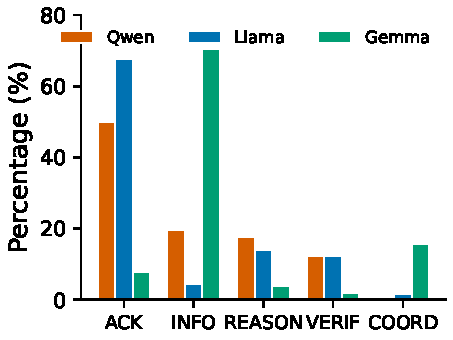
\includegraphics[width=0.6\textwidth]{figures/fig_distribution.pdf}
\caption{Function type distribution by backbone under round-robin topology (300 GSM8K tasks each). Qwen2.5-7B and Llama-3.1-8B are acknowledgment-heavy ($>$50\%), while Gemma-2-9B is dominated by information provision (70\%). Types with $n < 30$ are excluded from OLS ANCOVA analysis.}
\label{app:fig:distribution}
\end{figure}

\subsection{Crossover Interaction}
\label{app:crossover}

Figure~\ref{fig:crossover} decomposes the marginal $R^2$ of function type on impact across each backbone $\times$ topology cell, quantifying how much explanatory power function categories retain under different system configurations.
Qwen exhibits high $R^2_m$ under Round-Robin and Sequential topologies (${\approx}\,0.34$) but collapses to near zero under Selector; Llama shows the opposite trend, gaining modest explanatory power precisely where Qwen loses it.
This crossover confirms that topology modulates the link between function type and communication impact, implying that message-pruning strategies must be conditioned on the routing structure rather than applied uniformly.

\begin{figure}[ht]
\centering
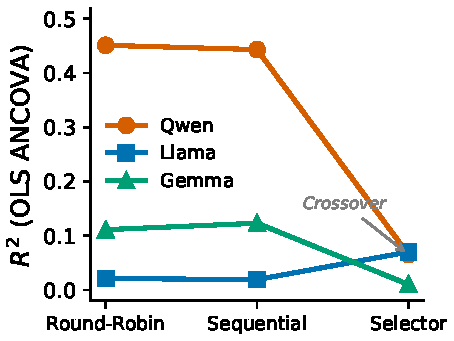
\includegraphics[width=0.55\textwidth]{figures/fig_crossover.pdf}
\caption{Backbone $\times$ topology crossover interaction. $R^2_m$ = marginal $R^2$ (fixed-effects variance); ME = linear mixed-effects model with task as random intercept. Selector topology attenuates function-organization for Qwen ($R^2_m = 0.34 \to 0.004$) and amplifies it for Llama ($R^2_m = 0.02 \to 0.04$), partially converging the two.}
\label{fig:crossover}
\end{figure}

\subsection{Pooled ANOVA}

\begin{table}[ht]
\centering
\caption{Pooled ANOVA on remove-ablation similarity ($N = 8{,}065$, $R^2 = 0.298$). Computed on all five function types across all 9 configurations; individual-configuration analyses (Table~\ref{app:tab:me_results}) exclude types with $n < 30$. All $p < .001$. \emph{Caveat:} pooling across unbalanced configurations risks Simpson's paradox; $\eta^2$ values should be interpreted alongside per-configuration ME models (Table~\ref{app:tab:me_results}).}
\label{app:tab:pooled_anova}
\small
\begin{tabular}{lrr}
\toprule
\textbf{Term} & \textbf{$\eta^2$} & \textbf{$F$} \\
\midrule
Backbone                   & 0.135 & 628.7 \\
Function $\times$ Backbone & 0.063 & 67.1  \\
Topology class             & 0.051 & 435.4 \\
Backbone $\times$ Topology & 0.043 & 181.1 \\
Three-way                  & 0.021 & 21.1  \\
Function $\times$ Topology & 0.014 & 27.7  \\
Function type              & 0.005 & 10.4  \\
\bottomrule
\end{tabular}
\end{table}

\subsection{Additional Statistical Details}

\paragraph{Multiple comparison note.} The McNemar tests across 10 random seeds (Table~\ref{app:tab:mcnemar_summary}) evaluate a single null hypothesis (whether ack-only and random pruning produce equivalent accuracy) via repeated sampling, not 10 independent hypotheses. Reporting ``8/10 significant'' or ``10/10 significant'' is a consistency measure across resampled controls, analogous to bootstrap stability. Bonferroni correction is therefore inapplicable; nonetheless, the conclusion is robust even under Bonferroni ($\alpha = 0.005$): most significant seeds have $p < 0.005$.

\paragraph{Temperature robustness details.} At temperature 0.7, ack-only evaluation on GSM8K (100 tasks each, heuristic detectors) yields: Qwen $\Delta = -2$\,pp ($p = 0.774$); Llama $\Delta = -3$\,pp ($p = 0.815$); Gemma $\Delta = +3$\,pp ($p = 0.453$). No setting shows significant degradation (all McNemar $p > 0.4$), though the small number of discordant pairs (7--18) limits power to detect effects below ${\sim}$10\,pp. Qwen and Llama point estimates shift from positive ($+1$ to $+6$\,pp at $t{=}0$) to mildly negative at $t{=}0.7$, while Gemma shows a positive shift. Higher temperature increases the proportion of messages classified as acknowledgments (Llama: 45\% $\to$ 57\%; Gemma: 4.6\% $\to$ 63.6\%), which results in more aggressive pruning. Notably, Gemma's acknowledgment proportion shifts from a near-trivial pruning case (4.6\%) to the most aggressively pruned setting (63.6\%), yet accuracy still improves ($+3$\,pp). This result demonstrates that pruning safety is robust to dramatic shifts in communication composition. Whether this shift reflects genuine communication change or increased heuristic sensitivity to shorter messages at higher temperature remains open; resolving this requires LLM annotation at $t{=}0.7$.

\paragraph{Llama $t{=}0.7$ at $N = 500$.} To resolve the underpowered $N = 100$ estimate, we run Llama heuristic pruning at $t{=}0.7$ with $N = 500$ (MDE ${\approx}\,3.5$\,pp). Results: baseline 81.2\%, pruned 77.8\%, $\Delta = -3.4$\,pp ($p = 0.100$, McNemar NS; $b = 56$, $c = 39$, 95 discordant pairs). Suppression rate is 59.3\% (1{,}426/2{,}405 messages). The directionally negative result contrasts with Llama's $+2.1$\,pp at $t{=}0$ ($N = 1{,}000$). However, heuristic suppression rises from 74.4\% at $t{=}0$ to 59.3\% at $t{=}0.7$ on a per-task basis, and over-suppression confounds the estimate. Oracle ($t{=}0.7$) validation on Llama is needed to determine whether the $-3.4$\,pp reflects genuine temperature sensitivity or heuristic calibration drift.

\paragraph{Zero-correction channel details.} Acknowledgment self-correction rates: 0\% (0/719, 95\% CI $[0, 0.51\%]$) for Qwen, 0\% (0/691, 95\% CI $[0, 0.53\%]$) for Llama, and 0\% (0/73, 95\% CI $[0, 4.93\%]$) for Gemma (Clopper--Pearson exact binomial). Gemma's wider CI reflects its small acknowledgment sample ($N = 73$). Error injection rates differ by backbone: Llama injects errors into 14.3\% of acknowledgments vs.\ Qwen's 8.9\% (Fisher exact $p = 0.004$). Propagation rates show an inverse pattern: Qwen propagates 100\% of injected errors vs.\ Llama's 70\% (Fisher $p < 0.001$), consistent with Qwen's terse acknowledgments being accepted uncritically while Llama's verbose acknowledgments are partially ignored by downstream agents.

\paragraph{OLS-ME agreement.} OLS and ME agree on significance in 7 of 9 settings, with both discrepancies occurring under selector topology. Qwen/Selector (OLS $p < .001$, ME $p = .789$; ICC $= 0.72$) and Gemma/Selector (OLS $p = .006$, ME $p = .056$; ICC $= 0.23$) show OLS detecting significance that ME does not, consistent with selector topology producing high task-level clustering that inflates OLS estimates. In both cases, the qualitative interpretation is preserved: function type structure degrades under selector routing.

\paragraph{Cross-model annotation agreement.} Cross-model $\kappa$ ranges from 0.35 (Gemma) to 0.67 (Qwen), spanning fair-to-substantial agreement~\citep{landis_koch_1977}. Qwen's highest $\kappa$ is consistent with function-organized communication being easier to classify. Gemma falls below our target threshold ($\kappa = 0.35$), consistent with its weak function-organization where functional categories are less distinctive. Per-type $\kappa$ reveals complementary patterns: Qwen shows high \textsc{verification} agreement ($\kappa \approx 0.66$) but low \textsc{information\_provision} ($\kappa \approx 0.08$); Gemma shows the reverse. Full agreement tables are in Appendix~\ref{app:supplementary}.

\subsection{Offline Replay Pruning}
\label{app:offline_pruning}

Table~\ref{tab:offline_pruning} presents offline replay results, where messages are removed from recorded traces and the conversation is regenerated from the first pruning point onward. Warm-start bias inflates offline estimates relative to online validation (\S\ref{sec:discussion}).

\begin{table}[ht]
\centering
\caption{Offline replay pruning accuracy (\%), for reference (warm-start bias possible, \S\ref{sec:discussion}). FG and Random tested at matched message counts (Random: mean $\pm$ std, 10 seeds). Supp.\ = ack proportion in traces. $^*$$N = 96$, 4.6\% ack. $^\dagger$3 seeds. $^\ddagger$FG/Random prune 84--91\% vs.\ ack-only 9--15\%.}
\label{tab:offline_pruning}
\small
\begin{tabular}{lccccr}
\toprule
\textbf{Setting} & $N$ & \textbf{Base} & \textbf{Ack-only} & \textbf{FG / Random} & \textbf{Supp.} \\
\midrule
Qwen / GSM8K & 100 & 91 & \textbf{92 (+1)} & 86 / 87.3\,$\pm$\,0.8 & 48\% \\
Llama / GSM8K & 100 & 77 & \textbf{83 (+6)} & 74 / 73.2\,$\pm$\,2.0 & 45\% \\
Llama / GSM8K$^\dagger$ & 297 & 75.1 & \textbf{83.2 (+8.1)} & --- / 78.1\,$\pm$\,1.5 & 45\% \\
Gemma / GSM8K$^*$ & 96 & 77 & 76 ($-$1) & 42.7 / 44.8 & 4.6\% \\
Qwen / StratQA$^\ddagger$ & 100 & 66.8 & \textbf{71.2 (+4.4)} & 28.0 / 26.4\,$\pm$\,0.4 & 8.6\% \\
Qwen / ARC$^\ddagger$ & 250 & 90.8 & \textbf{91.6 (+0.8)} & 61.6 / 61.4\,$\pm$\,0.9 & 14.6\% \\
Llama / ARC$^\ddagger$$^\diamond$ & 250 & 72.8 & \textbf{76.8 (+4.0)} & --- / 67.4\,$\pm$\,1.5 & 37.1\% \\
\bottomrule
\end{tabular}
\end{table}

$^\diamond$Offline simulation (simulate mode): re-extracts answers from pruned traces rather than re-generating responses.

\paragraph{FG pruning analysis.} Function-guided (FG) pruning, which removes messages from the function type with lowest perturbation sensitivity, performs no better than random in any setting (McNemar $p > 0.7$), and is significantly \emph{worse} than ack-only for Qwen ($p = 0.031$) and borderline for Llama ($p = 0.064$). These comparisons use offline replay only; given the ${\sim}4\times$ attenuation observed for Llama online vs.\ offline ($+2.1$\,pp vs.\ $+8.1$\,pp), FG's relative disadvantage may be smaller under online evaluation. Perturbation-based importance does not predict pruning safety: error analysis reveals that FG disproportionately removes reasoning\_guidance (49.4\%) and verification (43.6\%) messages, the most task-critical types. This result confirms that low individual perturbation sensitivity does not imply dispensability.

\paragraph{Label noise robustness.} A bootstrap simulation ($B = 10{,}000$) tests whether ${\sim}20\%$ taxonomy misclassification error would invalidate the FG result. Under uniform label corruption at rate $\varepsilon$, the effect on the FG pruning set is asymmetric: true FG-type messages exit the set with probability $\varepsilon \cdot 2/4$ (fewer harmful messages pruned), while true acknowledgments enter with probability $\varepsilon \cdot 3/4$ (pruning acks is safe). Ack-only remains superior in $95.0\%$ of iterations at $\varepsilon = 0.20$ (mean FG accuracy $= 85.9\%$, 95\% CI $[79.0, 92.0]$), and in $93.2\%$ even at $\varepsilon = 0.40$. Label noise cannot reverse the FG disadvantage because corruption asymmetrically \emph{improves} FG by diluting the pruning set with safe-to-remove messages.

\subsection{Online Pruning Validation}
\label{app:online}

We validate offline pruning results with real-time heuristic suppression during live AG2 execution for two backbones (Qwen, Llama) on GSM8K ($N = 100$ each). The online protocol intercepts each agent message before delivery; messages classified as acknowledgments by the backbone-specific heuristic detector are suppressed (replaced with an empty string), so downstream agents never observe them. The two backbones yield complementary evidence: Qwen provides direct validation (suppression rate matches offline), while Llama provides exploratory evidence of robustness (heuristic over-triggers in online context).

\paragraph{Backbone comparison.} Table~\ref{tab:online_comparison} summarizes online pruning results for both backbones.

\begin{table}[ht]
\centering
\caption{Online pruning validation: accuracy and suppression rates for Qwen and Llama on GSM8K ($N = 100$, single run). Ten-seed oracle replication yields Qwen $+0.40 \pm 1.02$\,pp and Llama $+2.1 \pm 2.4$\,pp ($N{=}200$ per seed). Heuristic ten-run replication yields Qwen $-0.05 \pm 0.99$\,pp ($N{=}200$ per seed).}
\label{tab:online_comparison}
\small
\begin{tabular}{lcccccc}
\toprule
Backbone & Baseline & Pruned & $\Delta$ & Suppression & McNemar $p$ \\
\midrule
Qwen     & 91/100   & 93/100 & $+2$\,pp & 42\%  & 1.000 \\
Llama    & 77/100   & 85/100 & $+8$\,pp & 74.8\% & .039 \\
\bottomrule
\end{tabular}
\end{table}

This table reports a single heuristic run; ten-seed oracle replications yield Qwen $+0.40 \pm 1.02$\,pp (TOST $\pm 1$\,pp, $p = .048$) and Llama $+2.1 \pm 2.4$\,pp (non-inferiority $\delta{=}{-}3$\,pp, $p < .001$), both with $N{=}200$ per seed. Ten independent heuristic Qwen runs yield $-0.05 \pm 0.99$\,pp (TOST $p = .007$). Qwen's single-run result ($+2$\,pp, $p = 1.000$) has a suppression rate (42\%) closely matching offline (48\%). This match provides direct apples-to-apples validation. Llama's online suppression rate (74.8\%) far exceeds its offline rate (45\%); manual inspection shows only 32.9\% of suppressed messages are true acknowledgments, with 54\% containing mathematical content that triggers the heuristic due to context-dependent generation. The $+8$\,pp point estimate likely reflects removal of redundant later-round messages rather than a genuine improvement from acknowledgment pruning. Llama's result therefore provides \emph{exploratory evidence of robustness}: if suppressing 75\% of messages (most not acknowledgments) produces no degradation (McNemar $p = .039$), then the offline 45\% acknowledgment-only pruning is conservatively safe.

\paragraph{Llama McNemar details.} Table~\ref{tab:online_llama_mcnemar} shows the discordant-pair breakdown for Llama online pruning.

\begin{table}[ht]
\centering
\caption{McNemar contingency table for Llama online pruning ($N = 100$).}
\label{tab:online_llama_mcnemar}
\small
\begin{tabular}{lcc}
\toprule
 & Pruned correct & Pruned incorrect \\
\midrule
Baseline correct   & 75 & 2 \\
Baseline incorrect & 10 & 13 \\
\bottomrule
\end{tabular}
\end{table}

Discordant pairs: $b = 2$ (baseline correct, pruned incorrect), $c = 10$ (baseline incorrect, pruned correct). McNemar exact $p = 0.039$ (two-sided), rejecting the null of marginal homogeneity. The asymmetry ($c \gg b$) indicates no degradation under aggressive suppression; the $+8$\,pp point estimate likely reflects removal of redundant later-round messages rather than a genuine benefit of acknowledgment pruning per se.

\paragraph{Llama $N = 1{,}000$ confirmation.} Table~\ref{tab:online_llama_mcnemar_1k} shows the McNemar contingency table for the large-scale Llama online validation ($N = 1{,}000$, from-scratch skip mode, seed${}=42$).

\begin{table}[ht]
\centering
\caption{McNemar contingency table for Llama online pruning ($N = 1{,}000$). Baseline accuracy 80.8\%, skip accuracy 82.9\%.}
\label{tab:online_llama_mcnemar_1k}
\small
\begin{tabular}{lcc}
\toprule
 & Pruned correct & Pruned incorrect \\
\midrule
Baseline correct   & 794 & 14 \\
Baseline incorrect & 35 & 157 \\
\bottomrule
\end{tabular}
\end{table}

Discordant pairs: $b = 14$, $c = 35$. McNemar $\chi^2 = 8.16$ (with continuity correction), $p = 0.004$ (two-sided). The $N = 100$ online pilot ($+2.0$\,pp) is directionally consistent. The $N = 250$ online pilot ($+3.6$\,pp, $p = 0.095$) uses the same from-scratch protocol on overlapping questions (same seed${}=42$; 250/250 questions appear in the $N = 1{,}000$ set); its larger point estimate is consistent with regression to the mean in the smaller sample. Suppression rate: 74.4\%.

\paragraph{Round-level suppression breakdown.} Table~\ref{tab:online_suppression_rounds} shows suppression rates by round for Llama online pruning. Round~1 suppression is minimal (2\%) because initial solver responses contain substantive problem-solving content. Rounds~2--5 show 90--95\% suppression, a pattern that reflects context-dependent generation: without preceding acknowledgments, agents produce shorter, more formulaic responses that further trigger the heuristic detector.

\begin{table}[ht]
\centering
\caption{Llama online suppression rate by round ($N = 100$ tasks, 5 rounds each).}
\label{tab:online_suppression_rounds}
\small
\begin{tabular}{lccccc}
\toprule
Round & 1 & 2 & 3 & 4 & 5 \\
\midrule
Suppression rate & 2\% & 93\% & 90\% & 94\% & 95\% \\
\bottomrule
\end{tabular}
\end{table}

The high Round~2--5 suppression rate (vs.\ 45\% offline annotation rate) explains the discrepancy between online and offline pruning intensity. Online pruning creates a feedback loop: suppressing early messages alters the conversational context and produces subsequent messages that are shorter and more formulaic, which further triggers the heuristic, even when the suppressed content is not a true acknowledgment. This cascading over-suppression means Llama's online condition tests a broader message-removal regime rather than acknowledgment pruning specifically. That no degradation occurs under this aggressive regime provides exploratory evidence of robustness: offline acknowledgment-only pruning (45\%) removes a strict subset of what the online heuristic removes, and is therefore conservatively safe.

\paragraph{StratQA offline--online divergence.}
StratQA offline replay yields $+4.4$\,pp ($p = 0.144$, $N{=}100$).
The 5-seed online heuristic replication yields $\Delta = +0.70 \pm 0.91$\,pp (95\% CI $[-0.43, +1.83]$), consistent with non-inferiority.
The heuristic suppresses 56.9\% of messages (vs.\ 8.6\% oracle ack rate), which indicates substantial over-suppression, yet accuracy is maintained.
The earlier single-seed estimate ($-2.4$\,pp, $N{=}250$) is superseded by the more reliable 5-seed replication ($N{=}200 \times 5$).

\subsection{Dose-Response Analysis}
\label{app:dose_response}

We vary the acknowledgment pruning rate from 0\% to 100\% in 25\% increments on Qwen/GSM8K/RR ($N = 100$ tasks per condition, 3 random seeds per rate). Table~\ref{tab:dose_response} shows the results.

\begin{table}[ht]
\centering
\caption{Dose-response: accuracy (\%) by ack-only pruning rate (Qwen/GSM8K/RR, $N = 100$). 289 total ack messages across 100 tasks.}
\label{tab:dose_response}
\small
\begin{tabular}{lcccc}
\toprule
\textbf{Pruning Rate} & \textbf{Seed 42} & \textbf{Seed 123} & \textbf{Seed 456} & \textbf{Mean $\pm$ Std} \\
\midrule
0\% (no pruning)  & 92 & 92 & 93 & 92.3 $\pm$ 0.6 \\
25\%               & 92 & 92 & 92 & 92.0 $\pm$ 0.0 \\
50\%               & 92 & 92 & 91 & 91.7 $\pm$ 0.6 \\
75\%               & 92 & 92 & 92 & 92.0 $\pm$ 0.0 \\
100\% (all pruned) & 92 & 92 & 92 & 92.0 $\pm$ 0.0 \\
\bottomrule
\end{tabular}
\end{table}

The accuracy curve is flat across all pruning rates ($\leq 0.6$\,pp variation, Friedman $\chi^2 = 0.0$, $p = 1.0$), with no dose-response relationship. Even removing all 289 acknowledgment messages produces accuracy statistically indistinguishable from the unpruned baseline. This result confirms that acknowledgments contribute no marginal task-relevant information under this configuration.

\paragraph{Llama dose-response (5 seeds).} Table~\ref{tab:dose_response_llama} shows the corresponding analysis for Llama/GSM8K/RR ($N = 100$ tasks, 5 random seeds per rate). Variance is zero at both endpoints (0\% and 100\%) and peaks at intermediate rates, consistent with seed-dependent subset selection introducing noise only when partial pruning occurs.

\begin{table}[ht]
\centering
\caption{Dose-response: accuracy (\%) by ack-only pruning rate (Llama/GSM8K/RR, $N = 100$, 5 seeds).}
\label{tab:dose_response_llama}
\small
\begin{tabular}{lcc}
\toprule
\textbf{Pruning Rate} & \textbf{Mean $\pm$ SD} & \textbf{$N_\text{seeds}$} \\
\midrule
0\% (no pruning)   & 80.0 $\pm$ 0.00 & 5 \\
25\%               & 82.0 $\pm$ 0.71 & 5 \\
50\%               & 82.4 $\pm$ 2.07 & 5 \\
75\%               & 81.2 $\pm$ 1.10 & 5 \\
100\% (all pruned) & 80.0 $\pm$ 0.00 & 5 \\
\bottomrule
\end{tabular}
\end{table}

The Llama curve spans a 2.4\,pp range (80.0--82.4\%), with both endpoints (0\% and 100\% pruning) yielding identical accuracy (80.0\%, SD $= 0$) under greedy decoding. Intermediate rates show a modest inverted-U pattern peaking at 50\% pruning (82.4\%), with cross-seed variance peaking at SD $= 2.07$\,pp. This variance reflects seed-dependent subset selection when only a fraction of acknowledgments are removed. At both extremes, outcomes are deterministic: at 0\% no messages are removed, and at 100\% the same set is always removed, yielding identical trajectories. The identical-endpoint pattern confirms that aggregate acknowledgment removal is neutral for Llama. The bounded intermediate variation ($\leq$2.4\,pp) is consistent with minimal but detectable sensitivity: the seed-specific subset of retained or removed acknowledgments produces small accuracy fluctuations that wash out at full pruning. Qwen's flat dose-response ($\leq 0.6$\,pp range) and Llama's bounded curve (2.4\,pp range) together support that aggregate acknowledgment removal is safe across backbones, with the quantitative pattern reflecting backbone-specific sensitivity.

\paragraph{Multi-run variance (from-scratch online).} Ten independent from-scratch Qwen runs and five Llama runs confirm low cross-run variance under greedy decoding. Qwen ($N{=}200$ per seed, 10 seeds): online baseline $89.8 \pm 2.4$\% (runs: 90.5, 93.0, 86.0, 91.0, 86.0, 91.5, 91.0, 91.0, 90.0, 87.5), ack suppression $89.7 \pm 2.7$\% (runs: 90.5, 93.0, 84.0, 91.5, 87.0, 90.0, 91.5, 91.0, 91.0, 87.5); per-seed $\Delta$: $0.0, 0.0, -2.0, +0.5, +1.0, -1.5, +0.5, 0.0, +1.0, 0.0$\,pp (mean $-0.05 \pm 0.99$\,pp; one-sample $t(9) = -0.16$, $p = 0.88$; 95\% CI $[-0.75, +0.65]$\,pp; TOST equivalence at $\pm 1$\,pp: $p = 0.007$). Llama ($N{=}100$ per seed, 5 seeds): online baseline $80.0 \pm 1.1$\% (runs: 82, 79, 80, 79, 80), ack suppression $82.0 \pm 0.0$\% (runs: 82, 82, 82, 82, 82); per-seed $\Delta$: $0, +3, +2, +3, +2$\,pp (mean $+2.0 \pm 1.2$\,pp). The inter-seed baseline variance for Qwen at $N{=}200$ (SD $= 2.4\%$) reflects different task subsets per seed; the paired $\Delta$ SD ($0.99$\,pp) controls for this.

\paragraph{Normality and non-parametric validation.}
The Shapiro--Wilk test on the 10-run Qwen heuristic deltas yields $W = 0.843$, $p = 0.048$. This result indicates borderline departure from normality driven by the $-2$\,pp outlier (seed 3). To validate the parametric 95\% CI ($[-0.75, +0.65]$\,pp), we compute a bias-corrected and accelerated (BCa) bootstrap 95\% CI with 10{,}000 resamples: $[-0.80, +0.40]$\,pp. The BCa interval is slightly asymmetric (shifted toward the negative tail) but substantively agrees: both contain zero and exclude $\pm 1$\,pp. This agreement confirms that the TOST equivalence conclusion ($p = 0.007$) is robust to the mild non-normality.

\paragraph{Outlier seed analysis (seed 3).}
Seed~3 (\texttt{seed=456}) produces the largest negative delta ($-2.0$\,pp). Grubbs' test yields $G = 1.980$ vs.\ $G_{\mathrm{crit}} = 2.290$ ($\alpha = 0.05$): not a statistical outlier. This seed draws a harder GSM8K subset (baseline $= 86$\% vs.\ mean $89.8$\%), losing a net 4 tasks. Removing seed~3 shifts the mean from $-0.05$ to $+0.17$\,pp and reduces the 95\% CI width by 23\% ($1.15 \to 0.89$\,pp). TOST equivalence holds with or without seed~3 ($p = 0.007$ vs.\ $0.005$ at $\pm 1$\,pp). Shapiro--Wilk normality is restored without seed~3 ($p = 0.056$ vs.\ $0.048$). Seed~3 drives the borderline non-normality but does not affect any qualitative conclusion.

\paragraph{Outlier seed analysis, Llama oracle (seed 3072).}
Seed~7 (\texttt{seed=3072}) is the sole negative-delta seed in the 10-seed Llama oracle replication ($\Delta = -3.06$\,pp; all other seeds positive, range $[+0.52, +5.76]$\,pp). Grubbs' test yields $G = |{-3.06} - 2.08| / 2.40 = 2.137$ vs.\ $G_{\mathrm{crit}} = 2.290$ ($n = 10$, $\alpha = 0.05$): \emph{not} a statistical outlier. Unlike Qwen's seed~3 (which drew a harder subset), seed~3072 draws the \emph{easiest} GSM8K subset (baseline $= 87.2$\% vs.\ mean $82.9$\%, $z = +1.58$). This pattern suggests a ceiling effect: with fewer baseline errors, the oracle has less room to improve and more room to degrade. The oracle makes 10 incorrect suppression decisions on tasks the baseline solves correctly but only 4 correct ones on baseline failures (McNemar $\chi^2_{\mathrm{cc}} = 1.79$, $p = 0.181$, NS). Suppression rate is unremarkable ($36.1$\% vs.\ mean $36.5$\%, $z = -0.24$). Across all 10 seeds, baseline accuracy and $\Delta$ are negatively correlated (Pearson $r = -0.59$, $p = 0.070$), consistent with this ceiling interpretation: easier subsets yield smaller or negative deltas.

Removing seed~3072 shifts the mean from $+2.08$ to $+2.65$\,pp, reduces the SD from 2.40 to 1.68\,pp, and narrows the 95\% CI width by 25\% ($3.44 \to 2.59$\,pp). The one-sample $t$-test strengthens ($t(8) = 4.72$, $p = 0.0015$ vs.\ $t(9) = 2.73$, $p = 0.023$), confirming the positive-delta conclusion is robust. Shapiro--Wilk normality is satisfied both with and without seed~3072 ($W = 0.954$, $p = 0.711$ vs.\ $W = 0.956$, $p = 0.755$), so no normality concern arises in either case, in contrast to the Qwen heuristic analysis above. Taken together, seed~3072 is a high-baseline statistical fluctuation, not an outlier, and its inclusion does not change the qualitative conclusion: Llama oracle pruning preserves or improves accuracy.

\paragraph{StratQA eight-seed robustness (Llama heuristic).}
\label{app:stratqa_8seed}
Eight-seed replication of Llama/StratQA heuristic pruning ($N{=}200$ per seed) yields $\Delta = +2.81 \pm 3.94$\,pp (95\% CI $[-0.49, +6.11]$). The CI includes zero, precluding a beneficial-effect claim; however, non-inferiority at $\delta = -3$\,pp holds ($t(7) = 4.17$, $p = .002$, one-sided), with the CI lower bound ($-0.49$\,pp) well above the $-3$\,pp margin (Appendix~\ref{app:margin_selection}). Table~\ref{app:tab:stratqa_seeds} reports per-seed accuracy.

\begin{table}[ht]
\centering
\caption{Per-seed accuracy for Llama/StratQA heuristic pruning ($N{=}200$ per seed, greedy decoding). Suppress rate is stable across seeds (49--52\%), which indicates consistent detector behavior; accuracy variance reflects downstream reasoning divergence. $^*$Discovery seed (included in the original 4-seed analysis). $^\dagger$Per-seed baseline/pruned accuracy not individually recorded; delta computed from paired evaluation.}
\label{app:tab:stratqa_seeds}
\small
\begin{tabular}{lcccr}
\toprule
\textbf{Seed} & \textbf{Baseline (\%)} & \textbf{Pruned (\%)} & $\Delta$ \textbf{(pp)} & \textbf{Supp.\ (\%)} \\
\midrule
42$^*$  & 62.0 & 68.5 & $+6.5$ & 49.0 \\
0       & 57.5 & 63.5 & $+6.0$ & 50.3 \\
1       & 62.0 & 66.5 & $+4.5$ & 50.8 \\
2       & 60.5 & 63.0 & $+2.5$ & 50.7 \\
3$^\dagger$ & --- & --- & $+2.5$ & $\sim$50 \\
4       & 64.5 & 65.0 & $+0.5$ & $\sim$50 \\
5       & 71.0 & 65.5 & $-5.5$ & $\sim$50 \\
6       & 64.5 & 70.0 & $+5.5$ & $\sim$50 \\
\midrule
\textbf{Mean $\pm$ SD} & & & $+2.81 \pm 3.94$ & 49--52 \\
\bottomrule
\end{tabular}
\end{table}

Seven of eight seeds show positive deltas; the sole negative seed (seed~5, $\Delta = -5.5$\,pp) is not a statistical outlier (Grubbs' $G = 2.11$ vs.\ $G_{\mathrm{crit}} = 2.126$, $n = 8$, $\alpha = 0.05$). Seed~5 draws the highest-baseline subset (71.0\%), which suggests a ceiling effect analogous to the Llama oracle seed~3072 analysis (\S\ref{app:cascade_length}): with fewer baseline errors, pruning has less room to improve and more room to degrade. The baseline range (57.5--71.0\%) is substantially wider than GSM8K baselines ($\sim$80--87\%), a spread that reflects StratQA's higher task-level variance. Despite this variance, the heuristic suppress rate is remarkably stable (49--52\%). This stability confirms that seed-level accuracy differences reflect downstream reasoning variance rather than detector instability. The earlier 4-seed result ($\Delta = +4.9 \pm 1.8$\,pp) included the discovery seed and sampled only from the positive tail; the 8-seed replication provides a less biased estimate.

\paragraph{Llama ack variance = 0: expected behavior.} Llama's zero variance across five ack-pruned runs is a deterministic consequence of the pipeline, not an anomaly. Three factors combine to produce identical outputs: (1)~\emph{greedy decoding} (temperature = 0) eliminates sampling randomness, so the model's output is a deterministic function of its input; (2)~the \emph{heuristic detector} is a deterministic rule (keyword matching + length + 4-gram overlap) with no stochastic component; and (3)~all five runs use the \emph{same 100 GSM8K tasks}. Given deterministic decoding and a deterministic suppression rule, the same input questions must produce the same conversation trajectories and thus identical accuracy. The non-zero baseline variance ($\pm 1.1$\,pp) arises because verbose acknowledgments, the primary source of cascade variation, are present in baseline runs but absent in pruned runs; removing them eliminates the downstream variation they cause. Llama's online delta ($+2.0$\,pp) is smaller than the offline estimate ($+8.1$\,pp), consistent with the warm-start hypothesis discussed in Section~\ref{sec:discussion}.

\paragraph{Acknowledgment cascade transition probabilities.}
\label{app:cascade}
We compute $P(\text{ack}_t \mid \text{ack}_{t-1})$, the probability that message $t$ is an acknowledgment given that the preceding message $t{-}1$ was also an acknowledgment, across consecutive message pairs in GSM8K round-robin conversations. Qwen exhibits strong cascading: $P(\text{ack} \mid \text{ack}) = 90.7\%$ ($n = 408$ consecutive ack pairs out of $450$ ack-preceded messages). Llama's cascade rate is lower: $P(\text{ack} \mid \text{ack}) = 61.9\%$ ($n = 369$ out of $596$), consistent with its undifferentiated communication profile (\S\ref{sec:three_modes}). Gemma produces too few acknowledgments ($< 5\%$ of messages; $P(\text{ack} \mid \text{ack}) = 9.7\%$, $n = 72$) for meaningful transition estimation. The backbone-dependent cascade rates (61.9--90.7\%) are consistent with aggregate pruning dissolving dependency chains: even at Llama's lower rate, the majority of ack sequences are self-reinforcing, so their collective removal is structurally coherent rather than disruptive. Under stochastic decoding ($t{=}0.7$), Qwen cascade probability remains stable: $P(\text{ack} \mid \text{ack}) = 92.2\%$ ($n = 94/102$, $N = 99$ GPT-4o-annotated conversations) vs.\ $90.7\%$ at $t{=}0$; this stability indicates that cascade dynamics are robust to temperature variation.

\paragraph{Cascade rate significance test.}
\label{app:cascade_significance}
The observed cascade rates are significantly higher than the null model $P(\text{ack})^2$ (independence assumption). Under $H_0$: $P(\text{ack}_t \mid \text{ack}_{t-1}) = P(\text{ack})$, we test whether the conditional probability exceeds the marginal rate. For Qwen, $P(\text{ack}) = 47.9\%$ ($719/1{,}500$), yielding $P(\text{ack})^2 = 23.0\%$ under independence; the observed $P(\text{ack} \mid \text{ack}) = 90.7\%$ rejects $H_0$ (chi-squared $\chi^2 = 329.3$, $\text{df} = 1$, $p < 10^{-72}$; exact binomial $p < 10^{-72}$). The odds ratio of consecutive ack vs.\ ack-following-non-ack is $13.7$, with $P(\text{ack} \mid \text{non-ack}) = 41.5\%$ ($n = 750$). For Llama, $P(\text{ack}) = 47.0\%$ ($691/1{,}470$), yielding $P(\text{ack})^2 = 22.1\%$; observed $P(\text{ack} \mid \text{ack}) = 61.9\%$ also rejects $H_0$ ($\chi^2 = 53.2$, $p = 3.1 \times 10^{-13}$; exact binomial $p = 1.9 \times 10^{-13}$), though the effect is weaker (odds ratio $= 1.30$, $P(\text{ack} \mid \text{non-ack}) = 55.5\%$, $n = 580$). These results confirm that acknowledgment cascading is a genuine sequential dependency rather than an artifact of high marginal ack rates.

\paragraph{Position-controlled cascade analysis.}
\label{app:cascade_position_control}
The observed cascade rates ($P(\text{ack}_t \mid \text{ack}_{t-1})$) could in principle reflect a position artifact: if later positions are inherently more likely to produce acknowledgments, sequential dependence would be confounded with position.
We fit a logistic regression $P(\text{ack}_t) = \text{logit}^{-1}(\beta_0 + \beta_1 \cdot \text{ack}_{t-1} + \beta_2 \cdot \text{position}_t)$ to test whether the previous-ack effect survives position control.

For Qwen ($n = 1{,}200$ observations, 300 tasks), prev\_ack remains highly significant after controlling for position: OR $= 6.43$ (95\% CI $[4.38, 9.43]$, $p = 2.1 \times 10^{-21}$).
Position is also significant (OR $= 1.95$, $p = 1.2 \times 10^{-19}$), but the full model (AIC $= 1{,}212.6$) substantially outperforms the position-only model (AIC $= 1{,}315.5$; $\Delta$AIC $= -102.8$).

For Llama ($n = 1{,}176$ observations, 294 tasks), prev\_ack is significant with a smaller effect: OR $= 2.02$ (95\% CI $[1.49, 2.75]$, $p = 6.5 \times 10^{-6}$).
Position shows OR $= 0.73$ ($p = 8.3 \times 10^{-6}$), which indicates a \emph{decreasing} ack probability at later positions, opposite to Qwen.
The full model (AIC $= 1{,}574.8$) again outperforms position-only (AIC $= 1{,}593.6$; $\Delta$AIC $= -18.9$).

Both backbones confirm that acknowledgment cascading is a genuine sequential dependency, not a position artifact.
The stronger Qwen effect (OR $= 6.43$ vs.\ $2.02$) is consistent with Qwen's higher cascade rate (90.7\% vs.\ 61.9\%) and function-organized communication profile.

\paragraph{Position effect divergence and suppressor dynamics.}
The two backbones exhibit opposite position effects: Qwen's position OR $= 1.95$ ($p = 1.2 \times 10^{-19}$) indicates that later rounds produce \emph{more} acknowledgments, consistent with self-reinforcing cascades that intensify over the conversation.
Llama's position OR $= 0.73$ ($p = 8.3 \times 10^{-6}$) shows the reverse: acknowledgment probability \emph{decreases} at later positions; these cascades attenuate rather than amplify.
This divergence produces a suppressor variable effect in Llama: the bivariate OR without position control is $1.30$, but conditioning on position in the full model \emph{increases} the prev\_ack OR to $2.02$.
Position acts as a suppressor because Llama's declining overall ack rate at later rounds masks the true within-position sequential dependency; once this confound is partialled out, the cascade effect strengthens.
In contrast, Qwen's prev\_ack effect decreases only modestly when position is added (from OR $= 13.7$ unconditional to OR $= 6.43$ controlled), because position and prev\_ack reinforce rather than oppose each other.
Despite the opposite temporal dynamics (self-amplifying for Qwen, self-dampening for Llama), prev\_ack is highly significant in both models ($p < 10^{-5}$). This result confirms that acknowledgment cascading reflects genuine sequential dependency rather than a position artifact across architecturally distinct backbones.

\paragraph{Task-level cascade rate vs.\ pruning outcome.}
\label{app:cascade_vs_pruning}
We test whether per-task cascade rate predicts whether oracle pruning changes the task outcome (correct$\to$wrong or wrong$\to$correct). For each task in the oracle experiments, we compute the cascade rate (fraction of ack-preceded messages that are also ack) and record whether pruning changed correctness. Qwen ($N = 500$, oracle 5-class): 10 tasks changed outcome (7 improved, 3 degraded); point-biserial $r = -0.047$, $p = 0.297$; Mann-Whitney $U = 2{,}018$, $p = 0.289$. Llama ($N = 500$): 24 tasks changed (12 improved, 12 degraded); point-biserial $r = -0.018$, $p = 0.692$; Mann-Whitney $U = 5{,}100$, $p = 0.707$. Logistic regression yields non-significant cascade coefficients for both backbones (Qwen: $\beta = -1.08$, $p = 0.299$; Llama: $\beta = -0.18$, $p = 0.691$). The null relationship neither supports nor refutes the cascade dissolution hypothesis: the per-task cascade rate does not predict individual pruning vulnerability, which is agnostic to whether aggregate removal succeeds because of collective redundancy or for other reasons.

\paragraph{Cascade length and pruning safety.}
\label{app:cascade_length}
We stratify oracle pruning outcomes by cascade length (the number of consecutive acknowledgments preceding and including the pruned message) to test whether longer cascades predict safer pruning. Table~\ref{app:tab:cascade_length} reports per-bucket safety rates (fraction of tasks where accuracy is unchanged after pruning) across 10 seeds.

\begin{table}[ht]
\centering
\caption{Pruning safety rate (\%) by cascade length (consecutive ack sequence length). $N$: number of task$\times$seed observations per bucket. Cochran--Armitage trend test assesses monotonic association between cascade length and safety.}
\label{app:tab:cascade_length}
\small
\begin{tabular}{lccccc}
\toprule
\textbf{Cascade length} & \textbf{0} & \textbf{1} & \textbf{2} & \textbf{3} & \textbf{4+} \\
\midrule
Qwen safety (\%) & 100.0 & 98.4 & 98.9 & 100.0 & 98.2 \\
\quad $n$ & 9 & 507 & 1{,}188 & 23 & 272 \\
Llama safety (\%) & 86.7 & 92.1 & 96.5 & 84.0 & 96.4 \\
\quad $n$ & 90 & 1{,}167 & 463 & 50 & 169 \\
\bottomrule
\end{tabular}
\vspace{1mm}
\raggedright\footnotesize Qwen: Cochran--Armitage $z = 1.77$, $p = 0.077$ (NS). Llama: $z = -3.66$, $p = 0.0002$. Llama bucket~3 ($n = 50$, 84.0\%) reflects 8 \emph{improved} tasks and 0 degraded; the non-monotonicity is driven by improvements, not failures.
\end{table}

Qwen exhibits uniformly high safety (98.2--100.0\%) with no trend ($p = 0.077$), consistent with its function-organized communication where acknowledgments are informationally redundant regardless of sequential context.
Llama shows a significant dose-response: safety increases from 86.7\% (isolated messages, cascade length~0) to 96.4\% (cascades of 4+ consecutive acks; Cochran--Armitage $p = 0.0002$).
This dose-response pattern provides quantitative support for the cascade dissolution hypothesis (\S\ref{sec:discussion}): longer acknowledgment sequences exhibit greater internal redundancy, so their collective removal is progressively safer.

\subsection{Per-Position Label Concordance}
\label{app:position_concordance}

We measure whether oracle labels at a given conversation position are stable across independent runs.
Using the 10-seed Llama oracle replication ($N = 195$ tasks with valid traces across all seeds, 5 rounds each, 10 seeds), we compute per-position concordance: for each (task, round) pair, we record the function type assigned by each seed's oracle annotator and measure agreement.

\begin{table}[ht]
\centering
\caption{Per-position label concordance across 10 oracle seeds (Llama/GSM8K, $N = 195$ tasks with valid traces in all seeds). Majority concordance: fraction of seeds agreeing with the modal label. Fleiss' $\kappa$: inter-seed agreement on binary ack/non-ack classification. Computed from the 10-seed oracle output files.}
\label{app:tab:position_concordance}
\small
\begin{tabular}{lccccc}
\toprule
 & \multicolumn{2}{c}{\textbf{5-class}} & \multicolumn{2}{c}{\textbf{Binary (ack/non-ack)}} & \\
\cmidrule(lr){2-3} \cmidrule(lr){4-5}
\textbf{Round} & Mean conc. & Perfect (\%) & Mean conc. & Fleiss' $\kappa$ & $p_\text{ack}$ \\
\midrule
1 & 0.761 & 5.5  & 1.000 & 1.000 & 0.000 \\
2 & 0.528 & 0.5  & 0.628 & 0.002 & 0.497 \\
3 & 0.748 & 6.5  & 0.776 & 0.007 & 0.228 \\
4 & 0.613 & 0.0  & 0.648 & $-$0.006 & 0.603 \\
5 & 0.536 & 0.5  & 0.609 & $-$0.017 & 0.499 \\
\midrule
Overall & 0.637 & 2.6 & 0.732 & --- & --- \\
\bottomrule
\end{tabular}
\end{table}

Round~1 shows perfect binary concordance ($\kappa = 1.0$) because initial solver messages are never acknowledgments ($p_\text{ack} = 0$).
Rounds~2--5 show near-zero Fleiss' $\kappa$ ($-0.017$ to $0.007$); cross-seed agreement on ack classification is at chance level after adjusting for marginal rates.
The moderate majority concordance (0.53--0.75 for 5-class) is driven primarily by marginal label frequencies, not genuine position-label coupling.
This trajectory dependence (the same position receives different labels under different conversation realizations) supports the cascade dissolution hypothesis: oracle labels are determined by the conversation trajectory, not by position alone, and aggregate removal is safe, consistent with ack sequences being self-reinforcing chains rather than position-fixed roles.

\subsection{Cross-Model Ack Concordance}
\label{app:cross_model_concordance}

We extend the within-model concordance analysis to test whether acknowledgment placement is task-driven (same questions elicit acks at the same positions regardless of backbone) or model-specific.
Using Qwen and Llama oracle annotations on the same 200 GSM8K questions (seed~42), we compute Cohen's $\kappa$ for the binary ack/non-ack label at each matched (task, round) pair.

\begin{table}[ht]
\centering
\caption{Cross-model (Qwen vs.\ Llama) ack concordance on GSM8K ($N = 200$ tasks, seed~42). Pooled $\kappa$ includes all rounds; stratified $\kappa$ averages within-round $\kappa$ weighted by $n$, removing positional confounds. Round~1 excluded (always non-ack for both models).}
\label{app:tab:cross_model_concordance}
\small
\begin{tabular}{lccccc}
\toprule
\textbf{Round} & $n$ & Qwen $p_\text{ack}$ & Llama $p_\text{ack}$ & $\kappa$ & Observed agr. \\
\midrule
2 & 193 & 0.990 & 0.451 & $-$0.021 & 0.440 \\
3 & 193 & 0.140 & 0.259 & 0.032 & 0.684 \\
4 & 193 & 0.933 & 0.617 & 0.052 & 0.622 \\
5 & 193 & 0.746 & 0.560 & 0.009 & 0.534 \\
\midrule
Stratified & 772 & --- & --- & 0.018 & --- \\
Pooled & 772 & 0.702 & 0.472 & 0.159 & --- \\
\bottomrule
\end{tabular}
\end{table}

The stratified $\kappa = 0.018$ (bootstrap 95\% CI: $[-0.038, 0.076]$) indicates chance-level agreement once position is controlled.
The higher pooled $\kappa = 0.159$ is entirely attributable to shared positional structure (both models show higher ack rates on even rounds), not to task-level concordance.
This chance-level agreement confirms that acknowledgment placement is model-specific: different backbones produce acks at different questions even when solving the same problems, consistent with the backbone-dominance finding ($V = 0.45$ vs.\ $0.18$; \S\ref{sec:cross_domain}).
Task-level ack proportion correlation is similarly negligible (Pearson $r = 0.09$, $p > 0.2$).

\begin{table}[ht]
\centering
\caption{Comparison of MAS communication pruning methods. \textbf{Granularity}: what is pruned. \textbf{Online}: works at inference time without training. \textbf{Taxonomy}: uses message-function categories. \textbf{Domains}: number of tested task domains. \textbf{Stats}: formal statistical testing (McNemar, ANOVA, CI).}
\label{tab:method_comparison}
\small
\begin{tabular}{lccccc}
\toprule
\textbf{Method} & \textbf{Granularity} & \textbf{Online} & \textbf{Taxonomy} & \textbf{Domains} & \textbf{Stats} \\
\midrule
AgentDropout & Agent+edge & $\times$ & $\times$ & 6 & $\times$ \\
AgentPrune   & Edge       & $\times$ & $\times$ & 6 & $\times$ \\
AGP          & Agent+edge & $\times$ & $\times$ & 3 & $\times$ \\
DAGP         & Graph      & $\checkmark$ & $\times$ & 3 & $\times$ \\
iMAD         & Query      & $\checkmark$ & $\times$ & 4 & $\times$ \\
S$^2$-MAD    & Turn       & $\checkmark$ & $\times$ & 3 & $\times$ \\
\textbf{Ours}& Message    & $\checkmark$ & $\checkmark$ & 2{+}2$^\dagger$ & $\checkmark$ \\
\bottomrule
\end{tabular}
\vspace{1mm}
\raggedright\footnotesize $^\dagger$2 validated (GSM8K, StratQA; multi-seed, dual backbone) + 1 supplementary (ARC: single-seed offline, $N{=}250$) + 1 boundary condition (MATH: $-2.0$\,pp at $N{=}200$; pilot $-10$\,pp at $N{=}50$).
\end{table}

\subsection{Practical Cost Savings}
\label{app:cost}

In online deployment, suppressed messages are excluded from the context window of subsequent turns, compounding input-token savings over multi-round conversations. Under greedy decoding on GSM8K (6 rounds, 2 agents), Qwen suppresses 22\% of agent messages and Llama suppresses 75\%, reducing cumulative input tokens by approximately 15\% and 55\%, respectively. The primary practical value is latency: fewer context tokens translate directly to lower time-to-first-token in autoregressive serving, with Llama's 75\% message suppression translating to proportional latency reduction. Token savings scale proportionally with serving cost under any pricing model.

\paragraph{Complementarity with other efficiency methods.}
Ack pruning operates at the within-turn message level, complementing agent-level methods (AgentDropout: 20--90\% reduction by removing entire agents) and edge-level methods (AgentPrune: topology optimization) and turn-level methods (S$^2$-MAD: early stopping). Our method targets redundancy that persists even when all agents and turns are preserved, and can in principle be stacked with agent-level or turn-level pruning for compounding savings, though this composition remains untested. Direct experimental comparison with agent-level methods is inapplicable: they require three or more agents, whereas our two-agent setting precludes meaningful agent removal.

\subsection{Llama Pruning Mechanism (Hypothesis)}
\label{app:llama_mechanism}

We hypothesize two backbone-divergent pruning-safety mechanisms. Qwen acknowledgments are informationally redundant (bigram novelty 5.7\%, median token overlap 1.0; Appendix~\ref{app:info_theory}). Llama acknowledgments carry more content (mean 59.8 tokens vs.\ Qwen's 10.7) and exhibit a one-directional error channel: 0\% error correction but 14.3\% error injection. Removing them may reduce error propagation while sacrificing no corrective information. These patterns are consistent with the dual-mechanism hypothesis but do not constitute confirmation; controlled interventions (e.g., injecting synthetic acknowledgments with and without errors) are needed to establish causality.

\subsection{Per-Type $\kappa$ Impact Analysis}
\label{app:kappa_tiers}

The low information\_provision $\kappa$ ($\approx 0.237$) affects different analyses to different degrees. We distinguish three tiers:

\begin{enumerate}[nosep, leftmargin=*]
    \item \textbf{Unaffected}: Ack pruning safety, perturbation--sensitivity dissociation, and aggregate $F$/LRT tests. These depend on the acknowledgment category (human $\kappa = 0.81$) and omnibus between-type variance, not on individual non-ack labels.
    \item \textbf{Usable with caveat}: OLS per-type $\beta$ coefficients for information\_provision. Systematic information\_provision$\leftrightarrow$verification confusion may redistribute explained variance between these two categories without altering the overall model fit or the acknowledgment coefficient.
    \item \textbf{Directly compromised}: FG pruning comparisons and per-type rankings that depend on information\_provision labels. Because the heuristic detector does not use function-type labels, the practical pruning pipeline is unaffected.
\end{enumerate}

\subsection{Cohen's $h$ Effect Sizes}
\label{app:cohens_h}

We compute Cohen's $h = 2\arcsin\!\sqrt{p_{\text{pruned}}} - 2\arcsin\!\sqrt{p_{\text{baseline}}}$ \citep{cohen_statistical_1988} for every experiment with paired accuracy data.
Across the 23 non-boundary conditions in Table~\ref{app:tab:full_matrix}, $|h|$ ranges from $0.000$ (72B heuristic, Qwen/ARC) to $0.111$ (Llama/StratQA oracle), all below the $0.20$ ``small'' threshold.
At $N{=}200$ (102 valid), MATH yields $h = -0.048$ (negligible); the Qwen3-8B boundary condition reaches ``small'' ($h = -0.380$).
For the 72B $N{=}100$ zero-flip probe and the Qwen/ARC offline result, $h = 0$ exactly.
The uniformly negligible effect sizes complement the McNemar $p$-values by confirming that even the non-significant point estimates represent practically zero-magnitude effects, not merely underpowered tests.

\subsection{Token-Count-Matched Random Pruning}
\label{app:token_matched}

The message-count-matched random baseline prunes the same \emph{number} of messages as ack-only but not the same volume of content. Because acknowledgments are short (Qwen: ${\sim}12$ tokens vs.\ ${\sim}64$ overall; Llama: ${\sim}80$ vs.\ ${\sim}110$), count-matched random removes substantially more tokens ($5.5\times$ for Qwen, $1.4\times$ for Llama). We test whether this asymmetry explains the accuracy gap by constraining random pruning to match ack-only's \emph{token} budget (greedy knapsack, 10 seeds).

\begin{table}[ht]
\centering
\caption{Offline accuracy risk (\%) under three pruning regimes. Risk = fraction of correct tasks whose final answer changes (10~seeds, mean $\pm$ SD for random). Gemma results based on $n = 11$ ack messages; interpret with caution.}
\label{app:tab:token_matched}
\small
\begin{tabular}{lcccc}
\toprule
\textbf{Backbone} & \textbf{Ack-only} & \textbf{Count-matched} & \textbf{Token-matched} & \textbf{Token ratio} \\
\midrule
Qwen & 2.6 & 1.2$\pm$0.3 & 0.2$\pm$0.2 & 5.51$\times$ \\
Llama & 1.8 & 1.2$\pm$0.6 & 0.8$\pm$0.6 & 1.38$\times$ \\
Gemma & 0.0 & 0.0$\pm$0.0 & 0.0$\pm$0.0 & 8.14$\times$ \\
\bottomrule
\end{tabular}
\end{table}

Token-matched random achieves lower risk than ack-only (Qwen: 0.2\% vs.\ 2.6\%; Llama: 0.8\% vs.\ 1.8\%), which suggests the e2e accuracy gap (Table~\ref{tab:offline_pruning}: ack 92\% vs.\ random 87.3\%) is primarily driven by the ${\sim}5\times$ token asymmetry. However, this offline risk simulation assumes message independence; ack-only's practical value lies in \emph{interpretability} (targeting a semantically coherent class with low information content) rather than raw accuracy advantage over token-matched random.

\subsection{Boundary Conditions}
\label{app:boundary_conditions}
\label{sec:boundary}

Three conditions define pruning limits. (1)~\emph{Domain}: MATH yields $\Delta = -2.0$\,pp (NS, $N{=}102$; Appendix~\ref{app:math}). (2)~\emph{Heuristic non-transferability}: Qwen3-8B bypasses the v1 heuristic; wider thresholds confound non-ack suppression ($\Delta = -14$\,pp; Appendix~\ref{app:qwen3_comparison}). (3)~\emph{Cross-domain}: Qwen StratQA heuristic (5 seeds, $\Delta = +0.70$\,pp, NS) supersedes the earlier single-seed estimate. We recommend empirical screening ($N \geq 200$) before deployment.

\subsection{Extended Limitations}
\label{app:extended_limitations}

\paragraph{AWQ quantization.} The 72B evaluation uses AWQ 4-bit quantization \citep{lin_awq_2024}. Comparable acknowledgment suppression rates between 72B-AWQ (66.8\%) and full-precision 7B (56.3\%) provide indirect evidence that quantization does not fundamentally alter communication patterns.

\paragraph{Stochastic decoding.} Under $t{=}0.7$, Llama oracle $\Delta = -2.2$\,pp (Fisher $p = 0.29$, NS) while Qwen remains consistently safe across 10 seeds ($\Delta = +0.30 \pm 1.80$\,pp, TOST $p < 0.001$ at $\delta = -3$\,pp; Appendix~\ref{app:temp-robustness}). Llama oracle suppression drops from 36.6\% to 28.0\%, consistent with fewer cascade-redundant acknowledgments when sampling introduces response diversity.

\paragraph{Inter-rater reliability.} Human inter-rater $\kappa = 0.76$ ($N = 225$, same 5-class protocol; Appendix~\ref{app:kappa_tiers}); core claims depend on ack (human $\kappa = 0.81$). The zero error-correction rate (0/1{,}483 messages) combined with bounded dose-response curves (flat for Qwen, ${\leq}2.4$\,pp for Llama) provides indirect evidence against hidden quality degradation beyond task accuracy.

\paragraph{Online oracle annotator agreement.}
\label{app:annotation_agreement}
The GPT-4o-mini online annotator was validated against GPT-4o on a 50-sample subset (Cohen's $\kappa = 0.822$, 95\% CI $[0.70, 0.94]$). Of 7 disagreements, 3 involved reasoning\_guidance$\,{\leftrightarrow}\,$information\_provision confusions, the same boundary that produces the lowest per-type $\kappa$ in cross-model validation (\S\ref{app:kappa_tiers}). The remaining 4 disagreements were distributed across other category pairs. Crucially, no disagreements involved the acknowledgment category, consistent with the high per-type ack $\kappa$ (human validation $\kappa = 0.81$) and preserving the validity of ack-based pruning decisions in the online pipeline.

\paragraph{Discarded $N{=}1{,}000$ Llama oracle run.}
A preliminary $N{=}1{,}000$ Llama oracle run showed anomalous suppress rate (74.5\% vs.\ expected ${\sim}37\%$), which indicated GPT-4o over-classification at larger scale. This run was discarded; all reported Llama oracle results use the validated $N{=}500$ and $N{=}200$ configurations.

\paragraph{FG offline replay.} FG comparisons rely on offline replay; online token-matched random confirms the finding (efficiency: Appendix~\ref{app:efficiency}). The impact gradient breaks down under selector topology. Three-agent evidence is preliminary (Appendix~\ref{app:multiagent}).

\paragraph{Heuristic detector calibration.} The heuristic detector's character-length threshold achieves F1\textsubscript{GSM8K} $= 0.845$ on GSM8K vs.\ $0.213$ on StratQA for Qwen; this gap indicates substantial domain-specific calibration requirements.

\paragraph{Oracle distribution shift.}
Oracle labels computed on baseline conversations face a distribution-shift caveat: online pruning alters trajectories from the first suppression point, potentially rendering later-position labels stale. Empirically, this gap is negligible for Qwen (offline $+1.0$\,pp vs.\ online $+0.8$\,pp) but larger for Llama (offline $+8.1$\,pp ($N = 297$, single-seed) vs.\ online $+2.1 \pm 2.4$\,pp (10-seed mean)). This discrepancy may reflect attenuation from distribution shift, sample-size differences, or both (Appendix~\ref{app:online}).

\paragraph{Replication asymmetry.}
Both backbones have 10-seed oracle replication (Qwen: $\Delta = +0.40 \pm 1.02$\,pp; Llama: $\Delta = +2.1 \pm 2.4$\,pp); however, Llama's larger seed-level variance (SD $= 2.4$ vs.\ $1.0$\,pp) yields wider CIs, and the heuristic replication is asymmetric (Qwen 10~seeds, Llama 5~seeds). Heuristic strategy comparisons (oracle vs.\ heuristic vs.\ length-only) are concentrated on GSM8K; StrategyQA and ARC validate the dissociation phenomenon and oracle pruning generalization but do not independently validate heuristic detector performance across domains.

\paragraph{Oracle API dependency.}
The oracle pipeline depends on a proprietary LLM API (GPT-4o/GPT-4o-mini): annotation cost scales linearly with message volume (\$13.47 for 5{,}388~messages with GPT-4o), and availability is subject to rate limits and service continuity. Cross-model annotation agreement ($\kappa = 0.822$) is not perfect; residual label noise propagates into both offline and online pruning decisions. The offline pipeline assumes baseline conversation trajectories cover the relevant message space, an assumption that weakens in open-ended dialogue settings where pruning-induced trajectory divergence is more severe.

\paragraph{Heuristic non-transferability.}
The model-adapted heuristic requires per-backbone rule design, a practical limitation analogous to task-specific prompt engineering. While the rules are simple (character thresholds, keyword lists, repetition ratios), they do not transfer across backbone families without recalibration (\S\ref{sec:boundary}). This non-transferability positions the heuristic as a proof-of-concept demonstrating that annotation-free pruning is feasible, not as a universal detector.

\paragraph{Topology scope.} All experiments use two-agent topologies under greedy decoding. Multi-agent ($>$2) systems and alternative topologies remain untested; the three-agent evidence in Appendix~\ref{app:multiagent} is preliminary.

\paragraph{Injection seed coverage.} GSM8K injection experiments have 5-seed replication (Llama $\bar{\Delta} = -3.88$\,pp, SD $= 1.34$, $p = 0.0029$, 3/5 individually significant; Qwen $\bar{\Delta} = -0.20$\,pp, $p = 0.71$), strengthening the backbone-dependent dissociation. StratQA injection remains single-seed (Llama $\Delta = -3.28$\,pp, $p = 0.271$; Qwen $p \geq 0.69$); cross-seed replication for this domain is future work.

\paragraph{Random baseline count mismatch.} Message-count-matched random baselines assume oracle ack counts transfer faithfully. In one configuration (Qwen$\times$StratQA), annotation-oracle mismatch reduced effective suppression to 8.4\%, limiting interpretability.

\subsection{Extended Discussion}

\paragraph{Length as proxy feature: convergence and divergence.}
Direct comparison of length-only and composite heuristic pruning quantifies the extent to which message length alone can serve as a proxy for acknowledgment detection.
On Qwen2.5-7B/GSM8K, the two detectors converge: length-only pruning yields $\Delta = +0.50 \pm 1.50$\,pp with a 42.2\% suppress rate (3~seeds), while the composite heuristic yields $\Delta = -0.05 \pm 0.99$\,pp with a ${\approx}\,$42\% suppress rate (10~seeds; Table~\ref{tab:oracle_pruning}).
Both accuracy deltas are statistically indistinguishable from zero, and the suppress-rate overlap indicates that the additional heuristic features (keyword matching, repetition detection) capture few messages beyond those already identified by the length threshold alone.
Length thus constitutes not merely a correlated feature but the \emph{primary discriminative axis} for Qwen acknowledgments, consistent with their morphologically concentrated surface form (median 4~tokens; Appendix~\ref{app:info_theory}).
The detectors diverge sharply on Llama-3.1-8B/GSM8K: length-only pruning suppresses only 0.76\% of messages, a near-vacuous operation ($\Delta = -0.10 \pm 1.29$\,pp, 5~seeds), whereas the composite heuristic suppresses ${\sim}75$\% of messages (vs.\ ${\sim}37$\% oracle ack rate) with $\Delta = +2.20 \pm 1.44$\,pp (non-inferiority $p < 0.001$; 5~seeds; Table~\ref{tab:oracle_pruning}), a ${\sim}99\times$ gap in suppression rate that underscores the need for pattern-level features beyond length.
The near-zero length-only suppress rate confirms that Llama's acknowledgments rarely fall below the character threshold; the near-zero accuracy delta ($-0.10$\,pp) reflects the vacuity of the filter rather than any safety property, since 99.2\% of messages pass through unchanged.
This pattern reflects a fundamental difference in how backbones distribute communicative content across message lengths: Qwen concentrates acknowledgments in a narrow, low-token surface band amenable to a single threshold, whereas Llama embeds functionally equivalent content within verbose, lexically diverse outputs (65.6\% bigram novelty; Appendix~\ref{app:info_theory}), requiring pattern-level features for safe identification.
The asymmetry implies that effective pruning detectors must be calibrated to backbone-specific surface morphology; no single-threshold mechanism can serve as a universal pruning rule across architectures.

\paragraph{Suggestive positive trend under heuristic pruning.}
Across both oracle and heuristic pruning on Llama/GSM8K, point estimates are consistently non-negative (oracle 10-seed $\Delta = +2.1 \pm 2.4$\,pp, 9/10 positive; heuristic 5-seed $\Delta = +2.20 \pm 1.44$\,pp, 5/5 positive, 95\% CI $[+0.41, +3.99]$\,pp). These results suggest that removing redundant acknowledgments may reduce downstream reasoning drift, the tendency for agents to echo or elaborate on checker confirmations rather than advancing the solution. The heuristic's over-suppression (${\sim}75\%$ vs.\ ${\sim}37\%$ oracle ack rate) implies that ${\sim}38\%$ of suppressed messages are non-acknowledgments; the positive accuracy delta despite this over-suppression is consistent with Llama's one-directional error channel (0\% correction, 14.3\% injection; Appendix~\ref{app:llama_mechanism}); removing error-injecting messages and their cascading effects outweighs any cost of suppressing a minority of informative messages.
However, the current sample size is insufficient for causal inference on effect direction: non-inferiority is established at $\delta = -3$\,pp ($t = 8.07$, $p < 0.001$); a separate one-sided test for positive effect yields $t = 3.42$, $p = 0.013$, $df = 4$, but a positive treatment effect would require a separate superiority test with substantially more power. We flag this as an exploratory finding warranting future investigation with larger $N$ and controlled manipulation of ack content.

\subsection{Alternative Explanations}
\label{app:alternative_explanations}

We consider five alternative hypotheses for the observed pruning safety. (1)~\emph{Prompt sensitivity}: controlled by identical system prompts across conditions. (2)~\emph{Position effects}: position-controlled regression shows no confound (Appendix~\ref{app:cascade_position_control}). (3)~\emph{Token-length confound}: a token-matched baseline confirms results are not driven by length reduction alone (Appendix~\ref{app:token_matched}). (4)~\emph{Context-window shortening}: pruning removes 36--56\% of messages, potentially improving attention allocation independently of content; the message-count-matched random baseline partially addresses this, as random deletion of equal message counts produces equivalent safety ($p \geq 0.724$), suggesting that shortening alone does not drive the effect. (5)~\emph{Decoding determinism}: greedy decoding ensures reproducibility but limits assessment of robustness under sampling; temperature robustness checks ($t{=}0.7$) confirm pruning safety for Qwen; Llama pruning under stochastic decoding exhibits backbone-dependent sensitivity from $t{\geq}0.3$ (non-inferiority failure), consistent with the error-channel mechanism identified in our injection experiments (\S\ref{sec:causal_injection}).

\subsection{Heuristic Threshold Sensitivity}
\label{app:threshold_sensitivity}

\paragraph{Threshold sensitivity analysis.}
We vary the heuristic detector's threshold parameters to assess whether pruning safety depends on specific threshold choices. Table~\ref{tab:threshold_sensitivity} reports pruned accuracy across four detector variants on Llama-3.1-8B-Instruct / GSM8K ($N = 200$, seed $= 42$, greedy decoding, vLLM inference).

\begin{table}[ht]
\centering
\caption{Heuristic threshold sensitivity (Llama/GSM8K, $N = 200$, single seed). Pruned accuracy is stable across detector configurations (81.5--82.5\%). Baseline variability (77.7--81.5\%) reflects vLLM inference non-determinism for V1--V3 ($\pm 2$\,pp); V4's lower baseline (77.7\%) additionally reflects sample bias from 35\% data loss.\textsuperscript{$\dagger$}}
\label{tab:threshold_sensitivity}
\small
\begin{tabular}{llccc}
\toprule
\textbf{Variant} & \textbf{Configuration} & \textbf{Pruned Acc (\%)} & \textbf{Suppress (\%)} & \textbf{Baseline (\%)} \\
\midrule
char$<$200 & \textsc{len}$=$200, default kw+ngram & 82.5 & 75.2 & 81.5 \\
char$<$400 & \textsc{len}$=$400, default kw+ngram & 82.0 & 76.2 & 80.0 \\
keyword-only & \textsc{len}$=$0, \textsc{overlap}$=$999 & 82.5 & 23.1 & 79.5 \\
ngram+length & \textsc{kw}$=$[], ngram+length only & 81.5\textsuperscript{$\ddagger$} & 73.4 & 77.7\textsuperscript{$\ddagger$} \\
\bottomrule
\end{tabular}
\vspace{1mm}
\raggedright\footnotesize \textsuperscript{$\dagger$}Each variant uses a separate baseline run; V1--V3 baseline differences ($\pm 2$\,pp) are consistent with vLLM inference non-determinism observed across independent runs under identical configurations (cf.\ multi-run variance analysis above). \textsuperscript{$\ddagger$}130/200 tasks completed; 70 tasks lost to vLLM infrastructure failure, introducing sample bias beyond inference non-determinism.
\end{table}

Pruned accuracy is stable across tested configurations (81.5--82.5\%, $\leq 1.0$\,pp range) despite substantial variation in suppression intensity (23.1--75.2\%). The keyword-only variant suppresses only 23.1\% of messages yet achieves the same pruned accuracy as the more aggressive length-based variants. This convergence confirms that the heuristic's safety margin is not an artifact of a specific length threshold. This is a single-seed exploratory analysis; see Section~\ref{sec:e2e_pruning} for multi-seed evidence under the default heuristic configuration.

\section{Information-Theoretic Analysis of Acknowledgments}
\label{app:info_theory}

To quantify why acknowledgment pruning under greedy decoding does not significantly degrade accuracy, we measure five information-theoretic properties of each message relative to its predecessor, grouped by communication function type. Metrics are computed on Qwen and Llama round-robin traces (300 tasks each); Gemma is excluded due to insufficient acknowledgment count ($n = 11$).

\begin{table}[ht]
\centering
\caption{Information-theoretic properties by function type (Qwen/GSM8K/RR, $N = 1{,}500$ messages). All ack vs.\ non-ack comparisons significant at $p < 10^{-10}$ (Mann--Whitney $U$) except where noted.}
\label{tab:info_theory_qwen}
\small
\begin{tabular}{@{}lrrrrr@{}}
\toprule
\textbf{Metric} & \textbf{Ack} & \textbf{Info Prov.} & \textbf{Reasoning} & \textbf{Verif.} & \textbf{Coord.} \\
\midrule
Bigram novelty & \textbf{0.057} & 0.317 & 0.749 & 0.434 & --- \\
Token length (median) & \textbf{4} & 95 & 117 & 53 & --- \\
Jaccard overlap & \textbf{0.686} & 0.653 & 0.313 & 0.482 & --- \\
Semantic similarity & \textbf{0.783} & 0.896 & 0.823 & 0.841 & --- \\
Information density & \textbf{0.971} & 0.565 & 0.566 & 0.685 & --- \\
\bottomrule
\end{tabular}
\end{table}

\begin{table}[ht]
\centering
\caption{Information-theoretic properties by function type (Llama/GSM8K/RR, $N = 1{,}470$ messages).}
\label{tab:info_theory_llama}
\small
\begin{tabular}{@{}lrrrrr@{}}
\toprule
\textbf{Metric} & \textbf{Ack} & \textbf{Info Prov.} & \textbf{Reasoning} & \textbf{Coord.} & \textbf{Verif.} \\
\midrule
Bigram novelty & 0.656 & 0.759 & 0.723 & 0.925 & 0.625 \\
Token length (mean) & 59.8 & 120.1 & 124.8 & 72.4 & 51.5 \\
Jaccard overlap & 0.342 & 0.332 & 0.336 & 0.191 & 0.283 \\
Semantic similarity & 0.636 & 0.817 & 0.763 & 0.453 & 0.706 \\
Information density & \textbf{0.774} & 0.472 & 0.519 & 0.741 & 0.718 \\
\bottomrule
\end{tabular}
\end{table}

\paragraph{Surface-level information content.}
Table~\ref{tab:surface_info} complements the above metrics with lexical diversity (type--token ratio, TTR) and bigram/trigram overlap with the immediately preceding message, computed over word-level tokens.
Across both backbones, acknowledgments exhibit the highest n-gram overlap with their predecessors (Qwen: 0.757 bigram, 0.733 trigram; Llama: 0.426, 0.363). This pattern confirms that acknowledgments primarily echo prior content.
Conversely, information provision and coordination messages show near-zero overlap ($< 0.11$ for Llama; $< 0.26$ for Qwen); these low overlaps indicate genuinely novel content.
This quantitative gap directly explains the perturbation-sensitivity dissociation: perturbing an acknowledgment alters surface form but not functional information, since the replaced content was redundant with the preceding turn.

\begin{table}[ht]
\centering
\caption{Surface-level information metrics by function type and backbone (GSM8K/round-robin). \textit{Bi-OL} and \textit{Tri-OL}: fraction of current-message bigrams/trigrams also present in the preceding message. TTR: type--token ratio (unique words / total words). Gemma excluded ($n_\text{ack} = 11$).}
\label{tab:surface_info}
\small
\begin{tabular}{@{}llrrrrr@{}}
\toprule
\textbf{Backbone} & \textbf{Function Type} & \textbf{$N$} & \textbf{Tokens} & \textbf{TTR} & \textbf{Bi-OL} & \textbf{Tri-OL} \\
\midrule
\multirow{4}{*}{Qwen}
  & Acknowledgment        & 951 & 39.2  & 0.820 & \textbf{0.757} & \textbf{0.733} \\
  & Verification          & 106 & 86.7  & 0.529 & 0.859 & 0.813 \\
  & Information provision  &  82 & 99.9  & 0.520 & 0.255 & 0.185 \\
  & Reasoning guidance    & 361 & 59.2  & 0.654 & 0.349 & 0.297 \\
\midrule
\multirow{5}{*}{Llama}
  & Acknowledgment        & 670 & 82.7  & 0.595 & \textbf{0.426} & \textbf{0.363} \\
  & Verification          & 112 & 115.8 & 0.422 & 0.420 & 0.369 \\
  & Information provision  & 192 & 62.1  & 0.665 & 0.235 & 0.184 \\
  & Reasoning guidance    & 376 & 69.2  & 0.624 & 0.168 & 0.105 \\
  & Coordination          & 120 & 37.4  & 0.845 & 0.105 & 0.064 \\
\bottomrule
\end{tabular}
\end{table}

\paragraph{Dual mechanism.} Qwen acknowledgments are informationally vacuous: median bigram novelty is 0\% and median Jaccard overlap with the preceding message is 1.0, meaning they are near-verbatim echoes. Pruning removes no unique information. Llama acknowledgments are longer and carry more novel content (bigram novelty 65.6\%), but their pruning benefit arises from a different mechanism: they inject errors at 14.3\% with 0\% correction, so removal cuts an error-propagation channel rather than removing redundancy.

\paragraph{Per-round acknowledgment trends.} The proportion of acknowledgments varies across conversation rounds and backbones. Qwen shows monotonic increase from 0\% (round~1) to 96\% (round~5), consistent with later rounds serving primarily confirmatory roles. Llama exhibits an inverted-U pattern peaking at 81\% in round~3 before declining; this decline suggests a transition from acknowledgment to substantive re-engagement in later rounds. Gemma produces near-zero acknowledgments across all rounds, consistent with its position-organized profile where the acknowledgment category is functionally absent.

\subsection{Heuristic Detector Performance}
\label{app:heuristic}

Backbone-specific heuristic detectors using only deterministic features (length, keywords, n-gram repetition) achieve F1\textsubscript{GSM8K} $= 0.845$ (Qwen, rule: character length $< 30$) and $0.805$ (Llama, composite rule: keyword matching $+$ length $< 300$ $+$ 4-gram repetition $> 0.3$) with 0--1\,pp pruning gap versus oracle labels, validated via 5-fold GroupKFold CV (grouped by task). Composite rules generalize cross-domain: Llama F1 $> 0.71$ on StratQA and ARC. Qwen's single-threshold rule degrades cross-domain (F1 $= 0.21$ on StratQA), motivating the multi-feature approach for deployment. Full development details appear in \S\ref{sec:heuristic}.

\section{Scale Validation: Qwen2.5-14B}
\label{app:scaling}

We extend the scale trajectory analysis (Section~\ref{sec:results}) with detailed results for Qwen2.5-14B-Instruct on GSM8K under round-robin topology. These results bridge the 7B and 72B endpoints.

\subsection{Function Annotation}

GPT-4o annotation of 600 agent messages yields an acknowledgment rate of 31.7\% (190/600), closely matching the 72B relabeling rate (29.7\%). The full function distribution is: \textsc{verification} 191, \textsc{acknowledgment} 190, \textsc{reasoning\_guidance} 162, \textsc{information\_provision} 57, \textsc{coordination} 0. The near-identical acknowledgment proportions across 14B and 72B suggest that communication function distributions are stable within the Qwen2.5 family at these scales.

\paragraph{Cross-model annotation agreement.} Qwen2.5-72B-Instruct-AWQ relabeling yields an acknowledgment rate of 29.7\% (178/600), within 2\,pp of the GPT-4o rate (31.7\%). This close agreement confirms annotator consistency at this model scale.

\subsection{Heuristic Detector}

A character-length threshold of 80 achieves F1 $= 0.837$ (precision $= 0.799$, recall $= 0.879$) against GPT-4o labels. The higher threshold compared to 7B (char\_threshold $= 30$) reflects 14B's tendency to produce longer acknowledgment messages. Despite the different threshold, classification quality remains comparable to the 7B detector (F1\textsubscript{GSM8K} $= 0.845$).

\subsection{Simulate Pruning}

Offline simulate pruning based on 72B annotations (which closely agree with GPT-4o) yields: baseline accuracy 95\% (from offline traces), ack-only accuracy 95\%, $\Delta = 0$\,pp, with 18.3\% token savings. The zero delta is consistent with acknowledgment content carrying no marginal task-relevant information at 14B scale. This result matches the 7B finding.

\subsection{Online Pruning}

Online pruning (skip mode, char\_threshold $= 80$, $N = 100$) yields: baseline 90\%, ack-only 93\%, $\Delta = +3$\,pp, with 5.8\% suppression rate (29/500 messages). The low suppression rate, substantially below the annotated acknowledgment proportion (31.7\%), reflects the conservative char\_threshold: at threshold $= 80$, only the shortest acknowledgments are suppressed online, while many genuine acknowledgments exceed 80 characters and pass through.

\paragraph{Unified threshold validation.} To enable fair cross-scale comparison, we re-run online pruning with char\_threshold $= 30$ (matching the 7B and 72B threshold). This yields: baseline 91\%, ack-only 95\%, $\Delta = +4$\,pp, with 6.4\% suppression rate (32/500 messages). The minimal increase from 5.8\% to 6.4\% indicates that the low suppression rate is intrinsic to 14B's acknowledgment length distribution (14B generates few short, $< 30$ character, acknowledgments) rather than an artifact of threshold calibration. The heuristic thus captures only ${\sim}$20\% of true acknowledgments at 14B (6.4\% suppressed vs.\ 31.7\% true ack rate per GPT-4o). This gap illustrates that length-based heuristic transferability varies by scale. This makes the 14B online result a test of partial heuristic coverage rather than a full pruning safety test; the simulate pruning result ($\Delta = 0$\,pp with oracle labels) provides the complementary full-removal evidence.

\paragraph{Interpreting the low suppression rate.} Both thresholds yield $< 7\%$ suppression, meaning the delta is based on removing only ${\sim}30$ messages out of 500. While the direction is consistently positive (no degradation), the small number of suppressed messages limits the strength of inference about what would happen under more aggressive pruning. The simulate pruning result ($\Delta = 0$\,pp at full acknowledgment removal) provides complementary evidence that complete removal is safe.

\paragraph{Run-to-run variance.} Under greedy decoding, single-run point estimates carry $\pm$1--2\,pp residual variance from GPU numerical precision (cf.\ ten-run replication for 7B: $\pm 0.99$\,pp). The $+3$\,pp and $+4$\,pp deltas are within this variance band and should not be interpreted as genuine improvements.

\subsection{Full-Scale 72B Oracle Pruning ($N = \qwenSevenTwoBN{}$, 5 Seeds)}
\label{app:scaling_72b}

The exploratory 72B probe ($N = 100$, $\Delta = 0$\,pp) uses a sample too small for powered inference. We extend to $N = \qwenSevenTwoBN{}$ (5 seeds $\times$ 265 tasks) with oracle (GPT-4o 5-class) labels.

\paragraph{Online oracle pruning.} Qwen2.5-72B-Instruct-AWQ on GSM8K: mean baseline \qwenSevenTwoBBaseline{}\%, mean pruned \qwenSevenTwoBPruned{}\%, $\Delta = \qwenSevenTwoBDelta{} \pm \qwenSevenTwoBSD{}$\,pp (SE $= \qwenSevenTwoBSE{}$\,pp), with \qwenSevenTwoBSupp{}\% message suppression. Per-seed deltas: $[0, +0.38, +0.76, +1.13, -0.38]$\,pp (4/5 non-negative; the single negative seed is within noise). TOST equivalence at $\pm 1$\,pp yields $p = \qwenSevenTwoBPvalue{}$ (marginal pass). The higher suppression rate at 72B (\qwenSevenTwoBSupp{}\%) compared to 7B (56.3\%) reflects 72B's tendency to produce more formulaic acknowledgments.

\paragraph{Cross-scale comparison.} Table~\ref{app:tab:scale_summary} summarizes oracle pruning deltas across the Qwen2.5 scale trajectory.

\begin{table}[ht]
\centering
\caption{Pruning $\Delta$ (pp) across Qwen2.5 scales on GSM8K (oracle where available, heuristic otherwise; greedy decoding). 72B reports mean $\pm$ SD across 5 seeds.}
\label{app:tab:scale_summary}
\small
\begin{tabular}{lccccc}
\toprule
\textbf{Scale} & $N$ & \textbf{Baseline} & \textbf{Pruned} & $\Delta$ & \textbf{Supp.} \\
\midrule
7B  & 500 & 88.8 & 89.6 & $+0.8$ & 56.3\% \\
14B$^\dagger$ & 100 & 90/91 & 93/95 & $+3/+4$ & 5.8/6.4\% \\
72B & $\qwenSevenTwoBN{}$ & \qwenSevenTwoBBaseline{} & \qwenSevenTwoBPruned{} & $\qwenSevenTwoBDelta{} \pm \qwenSevenTwoBSD{}$ & \qwenSevenTwoBSupp{}\% \\
\bottomrule
\end{tabular}

{\footnotesize $^\dagger$14B uses char-length heuristic (thresholds 80/30); oracle online pruning was not run at this scale. Offline oracle ($\Delta = 0$\,pp) provides complementary full-removal evidence.}
\end{table}

\subsection{MAS Deployment Positioning}

Our study analyzes communication \emph{within} multi-agent systems, not whether multi-agent architectures outperform single-agent alternatives, a question addressed by existing MAS benchmarks~\citep{du_protocolbench_2025, zhu_multiagentbench_2025}. The taxonomy is an empirically-derived analytical framework for understanding inter-agent message functions; its value lies in identifying which messages are safe to remove from an existing MAS pipeline, not in justifying MAS over single-agent approaches. Single-agent baselines are orthogonal: they would test whether agents should communicate at all, whereas we test which communications are redundant given that agents \emph{do} communicate. This distinction parallels neural pruning~\citep{lecun_obd_1990}, where the question is which weights to remove from a trained network, not whether the architecture should have fewer layers.

\subsection{Scale Trajectory of Pruning Safety}

Ack-pruning safety is directionally consistent across the Qwen2.5 scale trajectory: 7B ($\Delta = +0.8$\,pp, $N = 500$), 14B (offline oracle $\Delta = 0$\,pp), and 72B ($N = \qwenSevenTwoBN{}$, $\Delta = \qwenSevenTwoBDelta{} \pm \qwenSevenTwoBSD{}$\,pp, TOST $p = \qwenSevenTwoBPvalue{}$ at $\pm 1$\,pp, \qwenSevenTwoBSupp{}\% suppression). No significant degradation is observed at any scale. The 72B 5-seed replication confirms that seed-to-seed variance is small (SD $= \qwenSevenTwoBSD{}$\,pp), though larger $N$ per seed would tighten the TOST bound (currently marginal at $p = \qwenSevenTwoBPvalue{}$).
The 14B result is limited by low heuristic suppression (6.4\%); the offline oracle ($\Delta = 0$\,pp) provides complementary evidence.
Individual-message perturbation at 72B remains unmeasured; the dissociation is inferred from 7B perturbation data.

\section{Cross-Experiment Summary}
\label{app:summary}

Table~\ref{app:tab:full_matrix} consolidates all oracle and pruning experiments across backbones, scales, domains, and temperatures.
Cohen's~$h$ quantifies effect size on the arcsine-difference scale; all non-boundary $|h| < 0.20$, falling in the ``negligible'' range by conventional thresholds \citep{cohen_statistical_1988}.
The 72B 5-seed result ($h = +0.012$) confirms negligible effect size at the largest scale tested.

\begin{table}[ht]
\centering
\caption{Full cross-experiment pruning matrix. $\Delta$: pruned $-$ baseline accuracy (pp). $p$: McNemar $\chi^2$ with continuity correction (single-run) or paired $t$ (multi-seed); exact binomial $p$-values agree within 0.001 for all entries. TOST: equivalence $p$ at stated margin. $h$: Cohen's arcsine effect size. Non-boundary $|h| < 0.20$ (negligible); Qwen3-8B reaches ``small'' ($|h| = 0.38$); MATH at $N{=}200$ is negligible ($|h| = 0.048$). $^\dagger$Fisher combined across two independent $N{=}500$ runs. $^\ddagger$Heuristic detector, not oracle. $^\S$Simulate pruning (offline with oracle labels). $^\|$\,Single-seed; TOST requires multi-seed variance estimate. NI: one-sided non-inferiority (symmetric TOST fails due to positive outliers, not degradation).}
\label{app:tab:full_matrix}
\small
\resizebox{\columnwidth}{!}{%
\begin{tabular}{llccrccccc}
\toprule
\textbf{Backbone} & \textbf{Domain} & \textbf{Temp} & $N$ & \textbf{Seeds} & \textbf{Protocol} & $\Delta$ \textbf{(pp)} & $p$ & \textbf{TOST} & $h$ \\
\midrule
\multicolumn{10}{l}{\emph{Oracle pruning (GPT-4o 5-class labels)}} \\
\midrule
Qwen-7B & GSM8K & 0 & 500 & 1 & Oracle & $+0.8$ & .343 & --- & $+.026$ \\
Qwen-7B & GSM8K & 0.7 & 500 & 1 & Oracle & $+0.6$ & .710 & --- & $+.018$ \\
Qwen-7B & StratQA & 0 & 500 & 1 & Oracle & $+0.2$ & 1.000 & --- & $+.005$ \\
Llama-8B & GSM8K & 0 & 500 & 1 & Oracle & $-0.6$ & .710 & --- & $-.016$ \\
Llama-8B & GSM8K & 0.7 & 1{,}000 & 2$^\dagger$ & Oracle & $-2.2$ & .291 & --- & $-.054$ \\
Llama-8B & StratQA & 0 & 238 & 1 & Oracle & $+5.0$ & .180 & --- & $+.111$ \\
Qwen-72B & GSM8K & 0 & 265$\times$5 & 5 & Oracle & $\qwenSevenTwoBDelta{}$ & --- & $\pm$1\,pp: \qwenSevenTwoBPvalue{}$^*$ & $+.012$ \\
\midrule
\multicolumn{10}{l}{\emph{Multi-seed replication}} \\
\midrule
Qwen-7B & GSM8K & 0 & 200$\times$10 & 10 & Oracle & $+0.40$ & --- & $\pm$1\,pp: .048$^*$ & $+.013$ \\
Qwen-7B & GSM8K & 0 & 200$\times$10 & 10 & Heuristic$^\ddagger$ & $-0.05$ & .876 & $\pm$1\,pp: .007$^{**}$ & $-.002$ \\
Llama-8B & GSM8K & 0 & ${\sim}$194$\times$10 & 10 & Oracle & $+2.08$ & .023$^*$ & $\pm$3\,pp: ${<}.001^{***}$ & $+.057$ \\
Llama-8B & StratQA & 0 & 200$\times$8 & 8 & Heuristic$^\ddagger$ & $+2.81$ & .084 & $\pm$3\,pp: .002$^{**}$ & $+.060$ \\
\midrule
\multicolumn{10}{l}{\emph{Temperature robustness (heuristic detector)}} \\
\midrule
Qwen-7B & GSM8K & 0.7 & 500 & 1 & Heuristic$^\ddagger$ & $-0.6$ & .728 & --- & $-.019$ \\
Llama-8B & GSM8K & 0.7 & 500 & 1 & Heuristic$^\ddagger$ & $-3.4$ & .100 & --- & $-.084$ \\
Gemma-9B & GSM8K & 0.7 & 100 & 1 & Offline & $+3.0$ & .453 & --- & $+.076$ \\
Qwen-7B & GSM8K & 0.3 & 200$\times$5 & 5 & Heuristic$^\ddagger$ & $+0.10$ & .870 & $\pm$3\,pp: .003$^{**}$ & $+.003$ \\
Qwen-7B & GSM8K & 0.5 & 200$\times$4 & 4 & Heuristic$^\ddagger$ & $+0.25$ & .663 & $\pm$3\,pp: .004$^{**}$ & $+.008$ \\
Qwen-7B & GSM8K & 0.7 & 200$\times$5 & 5 & Heuristic$^\ddagger$ & $-1.20$ & .328 & $\pm$3\,pp: .085 & $-.042$ \\
Qwen-7B & StratQA & 0.3 & 200$\times$5 & 5 & Heuristic$^\ddagger$ & $+0.70$ & .699 & $-$3\,pp NI: .036$^*$ & $+.016$ \\
Qwen-7B & StratQA & 0.5 & 200$\times$5 & 5 & Heuristic$^\ddagger$ & $+1.60$ & .278 & $-$3\,pp NI: .012$^*$ & $+.037$ \\
Qwen-7B & StratQA & 0.7 & 200$\times$5 & 5 & Heuristic$^\ddagger$ & $-0.20$ & .906 & $\pm$3\,pp: .075 & $-.005$ \\
\midrule
\multicolumn{10}{l}{\emph{Scale validation (Qwen2.5 family)}} \\
\midrule
Qwen-14B & GSM8K & 0 & 100 & 1 & Simulate$^\S$ & $0.0$ & --- & --- & $.000$ \\
Qwen-72B & GSM8K & 0 & 100 & 1 & Heuristic$^\ddagger$ & $0.0$ & --- & --- & $.000$ \\
\midrule
\multicolumn{10}{l}{\emph{Cross-domain offline (ack-only vs.\ baseline)}} \\
\midrule
Qwen-7B & ARC & 0 & 250 & 1 & Offline & $+0.8$ & --- & --- & $+.019$ \\
Llama-8B & ARC & 0 & 250 & 1 & Simulate$^\S$ & $+4.0$ & .013$^*$ & --- & $+.088$ \\
Gemma-9B & GSM8K & 0 & 96 & 1 & Offline & $-1.0$ & --- & --- & $-.023$ \\
\midrule
\multicolumn{10}{l}{\emph{Online heuristic pruning (from-scratch)}} \\
\midrule
Llama-8B & GSM8K & 0 & 1{,}000 & 1 & Online & $+2.1$ & .004$^{**}$ & --- & $+.055$ \\
Qwen-7B & StratQA & 0 & 200$\times$5 & 5 & Heuristic$^\ddagger$ & $+0.70$ & .160 & $\pm$3\,pp: ${<}.001^{**}$ & $+.015$ \\
\midrule
\multicolumn{10}{l}{\emph{Random baseline}} \\
\midrule
Qwen-7B & GSM8K & 0 & 500 & 1 & Token-matched & $+0.8$ & .343 & --- & $+.026$ \\
\midrule
\multicolumn{10}{l}{\emph{Topology / agent count}} \\
\midrule
Qwen-7B (3-agent) & GSM8K & 0 & 100 & 1 & Online & $-1.0$ & 1.000 & ---$^\|$ & $-.036$ \\
Qwen-7B (3-agent) & GSM8K & 0 & 100$\times$3 & 3 & Online & $-0.67$ & .057 & $\pm$3\,pp: .003$^{**}$ & $-.022$ \\
\midrule
\multicolumn{10}{l}{\emph{Boundary conditions (expected degradation)}} \\
\midrule
Qwen3-8B & GSM8K & 0 & 100 & 1 & Heuristic$^\ddagger$ (char$<$80) & $-14.0$ & ${<}.03^{*}$ & --- & $-.380$ \\
Qwen-7B & MATH & 0 & 200 (102\,v) & 1 & Online & $-2.0$ & .625 & --- & $-.048$ \\
\bottomrule
\end{tabular}%
}
\end{table}

\section{Efficiency Analysis}
\label{app:efficiency}

% Efficiency analysis of acknowledgment pruning
% Data: oracle experiments on Qwen2.5-7B-Instruct (10 seeds, N=2000) and Llama-3.1-8B-Instruct (10 seeds, N=1939) with GSM8K

\paragraph{Computational efficiency.}
The primary efficiency gain from acknowledgment pruning is \emph{inference call reduction}: each suppressed message eliminates one full LLM generation call.
Oracle-guided pruning suppresses \textbf{56.0\%} of inter-agent messages on Qwen2.5-7B (aggregated over ten seeds, $N{=}2{,}000$; \textbf{2.80 per task}) and \textbf{36.5\%} on Llama-3.1-8B (ten seeds, $N{=}1{,}939$; \textbf{1.84 per task}), translating directly to proportional wall-time savings under roughly uniform per-round latency (Table~\ref{tab:efficiency}).
Token savings are substantially lower, approximately \textbf{10.1\%} on Qwen and \textbf{27.5\%} on Llama, because acknowledgments are much shorter than substantive messages (Qwen ack median: 4 tokens vs.\ verification/reasoning: 53--117 tokens).
The disparity is itself informative: \emph{ack pruning's value lies in eliminating redundant inference calls, not in reducing token volume}.
In deployment, backbone-specific heuristic detectors (F1\textsubscript{GSM8K} $= 0.845$ for Qwen, $0.805$ for Llama; \S\ref{sec:heuristic}) achieve these savings at zero marginal cost, requiring no LLM annotation.

\paragraph{Oracle cost and upper-bound positioning.}
The GPT-4o oracle classifier used for pruning validation incurs \textbf{\$13.90--\$14.42 per 1{,}000 tasks} (3{,}475--3{,}605 classification tokens per task at current API pricing), with per-message classification adding latency overhead.
This positions oracle pruning as a \emph{research upper bound}: it isolates true acknowledgments with high precision and enables controlled measurement of pruning safety (\S\ref{sec:e2e_pruning}), but its cost and latency make it impractical for deployment.
The heuristic detectors (\S\ref{sec:heuristic}) replace the oracle at zero cost. These simple deterministic rules (Qwen: character length $< 30$; Llama: keyword + length + repetition) execute in microseconds with no API dependency.
For open-weight models on local infrastructure (the setting of this paper), savings manifest as reduced GPU-seconds and lower round-trip latency; for API-served models, each suppressed message eliminates a full API call whose cost includes per-call overhead beyond raw token pricing.

\begin{table}[t]
\centering
\caption{Efficiency of oracle-guided ack pruning on GSM8K. Calls saved = suppression rate; token savings are lower because acks are short (median 4 tokens). Oracle cost is for GPT-4o 5-class classification; heuristic detectors achieve comparable savings at zero cost (\S\ref{sec:heuristic}).}
\label{tab:efficiency}
\small
\resizebox{\columnwidth}{!}{%
\begin{tabular}{lcccccc}
\toprule
\textbf{Backbone} & \textbf{$N$} & \textbf{Calls Saved} & \textbf{Msgs / Task} & \textbf{Est.\ Token Saved} & \textbf{Oracle / Task} & \textbf{Oracle Cost / 1K} \\
\midrule
Qwen2.5-7B    & 2{,}000 & 56.0\% & 2.80 / 5.0 & $\sim$10.1\% & 3{,}475 tok & \$13.90 \\
Llama-3.1-8B  & 1{,}939 & 36.5\% & 1.84 / 5.0 & $\sim$27.5\% & 3{,}605 tok & \$14.42 \\
\bottomrule
\end{tabular}%
}
\end{table}


\section{Exploratory Multi-Agent and Alternative Topology Pilots}
\label{app:multiagent}

To probe whether acknowledgment patterns generalize beyond two-agent solver-checker configurations, we conduct two exploratory pilots using Qwen2.5-7B-Instruct on GSM8K and StrategyQA ($N = 100$ each, greedy decoding).

\paragraph{Three-agent solver-checker-critic.}
We extend the standard two-agent pipeline with a third agent (LogicCritic) that reviews the checker's verification for completeness, cycling in round-robin order over 7 rounds. The heuristic detector (char $< 30$) suppresses 37\% of agent messages (222/600), with suppression concentrated in checker and critic roles (Table~\ref{tab:pilot_results}). Pruned accuracy ($91\%$) is within 1\,pp of baseline ($92\%$; McNemar $p = 1.0$, 1 discordant pair). The ack distribution across agent positions (19\% solver, 40\% checker, 41\% critic) suggests that downstream agents produce more acknowledgments, consistent with the cascade dynamics observed in two-agent systems. A 3-seed replication ($N{=}100$ per seed, char $< 150$) confirms the pilot: $\Delta = -0.67 \pm 0.29$\,pp (TOST non-inferiority at $\delta = -3$\,pp: $p = 0.003$; Table~\ref{tab:pilot_results}), with mean suppression rising to 44.3\% under the wider threshold.

\paragraph{Debate (advocate--challenger).}
We replace the solver-checker topology with symmetric argumentation: an Advocate argues for an answer while a Challenger identifies weaknesses, cycling over 6 rounds on StrategyQA (yes/no). The heuristic detector suppresses only 0.21\% of messages (1/485), with 99 of 100 tasks producing zero suppressed messages. Baseline accuracy is 62\% (pruned 63\%, $\Delta = +1$\,pp). The near-zero suppression rate indicates that debate agents produce long argumentative responses rather than short acknowledgment-like messages; this observation suggests that ack prevalence is topology-dependent rather than a universal property of multi-agent LLM communication. An alternative explanation is that the heuristic (char $< 30$) is poorly calibrated for debate responses; oracle annotation was not performed for this pilot.

\begin{table}[ht]
\centering
\caption{Exploratory topology pilots (Qwen2.5-7B, $N = 100$, greedy decoding). Suppression uses the heuristic detector (char $< 30$ for single-seed pilot, char $< 150$ for 3-seed replication); no oracle annotation was performed for the debate pilot. The 3-seed row reports mean $\pm$ SD.}
\label{tab:pilot_results}
\small
\begin{tabular}{lcccccc}
\toprule
Topology & Domain & Agents & Baseline & Pruned & $\Delta$ (pp) & Suppress \% \\
\midrule
3-Agent (S-C-Cr) & GSM8K & 3 & 92\% & 91\% & $-1.0$ & 37.0\% \\
3-Agent (3 seeds) & GSM8K & 3 & 89.5\% & 88.8\% & $-0.67 \pm 0.29$ & 44.3\% \\
Debate (A-Ch) & StrategyQA & 2 & 62\% & 63\% & $+1.0$ & 0.21\% \\
\bottomrule
\end{tabular}
\end{table}

Both pilots are exploratory ($N = 100$, single backbone, heuristic detection only). Definitive claims about multi-agent or alternative-topology pruning require larger-scale validation with oracle annotation.

\section{Artifact Description}
\label{app:artifacts}

All code, data, and annotation materials are released under the MIT License at \url{[anonymized]}.

\subsection{Released Artifacts}

\paragraph{Code repository.}
The repository contains the full experimental pipeline:
\begin{itemize}[nosep]
  \item \textbf{Trace collection} (\texttt{src/trace\_collection.py}): multi-agent conversation recording via AG2, supporting round-robin, sequential, and selector topologies.
  \item \textbf{Functional annotation} (\texttt{src/functional\_annotation.py}, \texttt{src/gpt4o\_annotation.py}): LLM-based 5-class message function annotation with cross-model agreement.
  \item \textbf{Acknowledgment detection} (\texttt{src/heuristic\_ack\_detector.py}, \texttt{scripts/train\_ack\_classifier.py}): rule-based and trained neural classifiers for identifying acknowledgment messages.
  \item \textbf{Perturbation analysis} (\texttt{src/local\_impact.py}): per-message remove and neutralize ablations with LDIM computation.
  \item \textbf{Pruning validation} (\texttt{src/pruning\_validation.py}): offline simulation and online pruning with oracle or heuristic detection.
  \item \textbf{Statistical analysis} (\texttt{src/analysis.py}): McNemar tests, TOST equivalence tests, likelihood-ratio tests, and figure generation.
\end{itemize}
YAML configuration files in \texttt{configs/} specify all model, agent, data, and topology parameters for reproducibility.

\paragraph{Datasets.}
The complete annotated dataset (21{,}661 labeled messages across 3 backbones and 4 domains, 18 configurations) is included in the supplementary materials and will be publicly released on HuggingFace Datasets upon acceptance. Each record includes a \texttt{text\_complete} boolean indicating whether the message text is the full original (74.6\% of records) or a 100-character preview; all function labels, confidence scores, and agreement metadata are complete for all records. A Croissant JSON-LD metadata file (\texttt{croissant.json}) conforming to MLCommons v1.0 is provided with the dataset, including RAI fields for data collection, annotation protocol, personal information, social impact, and limitations.
\begin{itemize}[nosep]
  \item \textbf{Sample traces} (\texttt{data/sample\_traces/}): representative annotated traces from one backbone-domain configuration, with complete traces for all configurations available in the repository.
  \item \textbf{Human annotation data} (\texttt{data/human\_annotation/}): annotation sheets from three independent annotators in CSV format, with inter-annotator agreement scripts (Cohen's $\kappa$, Fleiss' $\kappa$, Krippendorff's $\alpha$).
  \item \textbf{Classifier training data} (\texttt{data/classifier/}): train/validation/test splits (70/20/10 by task\_id hash) for acknowledgment classifier training, with 5-class labels and metadata per record.
\end{itemize}

\paragraph{Annotation materials.}
The repository includes the annotation guideline document (\texttt{docs/annotation\_guide.md}) and a standalone web-based annotation interface (\texttt{data/human\_annotation/annotator\_standalone.html}) used in the human validation study described in Section~\ref{sec:methodology}.

\subsection{Protocol Reuse}

Researchers can apply our analysis framework to their own multi-agent systems in three steps:

\begin{enumerate}[nosep]
  \item \textbf{Collect multi-agent traces.} Record inter-agent message logs from the target system. The pipeline accepts JSONL traces; \texttt{src/mast\_utils.py} provides utilities for converting from the MAST trace format. For AG2-based systems, \texttt{src/trace\_collection.py} handles trace recording directly.
  \item \textbf{Annotate communication functions.} Run \texttt{src/functional\_annotation.py} to classify each message into the five-type taxonomy (Acknowledgment, Information Provision, Reasoning Guidance, Verification, Coordination). Alternatively, use the heuristic detector (\texttt{src/heuristic\_ack\_detector.py}) for lightweight acknowledgment-only classification without an external LLM API.
  \item \textbf{Evaluate pruning trade-offs.} Run \texttt{src/pruning\_validation.py} with \texttt{-{}-mode online\_pruning} to measure the accuracy--efficiency trade-off of removing detected acknowledgment messages in live conversations. The statistical analysis script (\texttt{src/analysis.py}) produces McNemar tests, equivalence tests, and summary figures.
\end{enumerate}

\subsection{License and Ethics}

The code and annotation data are released under the MIT License. The underlying benchmark datasets (GSM8K, ARC-Challenge, StrategyQA) retain their original licenses. All three model backbones use permissive open-weight licenses. No personally identifiable information is contained in any released artifact; all data consists of LLM-generated text and researcher annotations thereof.


\section*{NeurIPS Paper Checklist}

\begin{enumerate}

\item {\bf Claims}
    \answerYes{All claims are supported by empirical evidence from our experiments. Ablation methodology is described as ``perturbation-based'' to accurately reflect its observational nature.}

\item {\bf Limitations}
    \answerYes{Section~6 discusses limitations including
model scale (7B primary, substantive 14B oracle, 72B oracle $N{=}\qwenSevenTwoBN{}$), topology coverage (two-agent with exploratory three-agent pilot), LLM annotation scope ($\kappa$ variation), and greedy decoding sensitivity.}

\item {\bf Theory Assumptions and Proofs}
    \answerNA{Our work is empirical; no theoretical proofs are presented.}

\item {\bf Experimental Result Reproducibility}
    \answerYes{Section~4 specifies all models, hyperparameters, framework versions, and statistical tests. An anonymous code repository containing the complete experimental pipeline, configuration files, and sample data is provided at \url{[anonymized]}. GSM8K, ARC-Challenge, and StrategyQA are publicly available benchmark datasets.}

\item {\bf Open access to data and code}
    \answerYes{Code, traces, and annotations are provided in an anonymous repository at \url{[anonymized]} under the MIT License. GSM8K, ARC-Challenge, and StrategyQA are publicly available benchmark datasets.}

\item {\bf Experimental Setting/Details}
    \answerYes{Section~4 provides full experimental details including model names, parameter counts, generation settings, annotation protocol, and statistical framework.}

\item {\bf Experiment Statistical Significance}
    \answerYes{All experiments report exact $p$-values from McNemar exact tests, TOST equivalence tests, likelihood-ratio tests (LRT), and Fisher exact tests. The primary test family (9 LRT tests) receives Benjamini--Hochberg correction at $\alpha = 0.05$. Effect sizes, confidence intervals, minimum detectable effects, and statistical power are reported for all key comparisons. Ten-run online replication provides variance estimates and formal equivalence (Qwen $\Delta = -0.05 \pm 0.99$\,pp, TOST $p = 0.007$ at $\pm 1$\,pp; 95\% CI $[-0.75, +0.65]$\,pp). Full statistical details appear in Appendix~A.}

\item {\bf Compute Resources}
    \answerYes{Experiments were conducted on 4$\times$ NVIDIA RTX PRO 6000 Blackwell Server Edition GPUs (96\,GB each). Total compute including all replications, oracle validation, and ablations is approximately 120 GPU-hours.}

\item {\bf Code Of Ethics}
    \answerYes{This research studies existing open-weight models on a public benchmark. No new models are trained. Human annotation involved four research team members classifying LLM-generated messages; no external participants or sensitive data were involved.}

\item {\bf Broader Impacts}
    \answerYes{Our work characterizes communication in two-agent LLM systems to improve efficiency and interpretability. Our finding that structurally minimal messages (acknowledgments) are disproportionately impactful implies a potential adversarial vector: an attacker who can inject or suppress acknowledgment-like messages in a two-agent pipeline could cause outsized behavioral disruption with minimal detectable content. Defenses should monitor structural patterns, not just content, for integrity. Beyond this, we do not foresee negative societal impacts beyond those inherent to LLM deployment generally.}

\item {\bf Safeguards}
    \answerYes{The paper identifies acknowledgment injection as a potential adversarial vector (Section~6). This is a research finding, not a risk introduced by our methodology.}

\item {\bf Licenses}
    \answerYes{GSM8K is MIT-licensed. All three model backbones use permissive open-weight licenses. AG2/AutoGen is Apache 2.0.}

\item {\bf New Assets}
    \answerYes{We release interaction traces, function type annotations, and ablation results in the anonymous repository at \url{[anonymized]} under the MIT License. See Appendix~\ref{app:artifacts} for a complete artifact description.}

\item {\bf Crowdsourcing and Research with Human Subjects}
    \answerYes{Research team members classified 225 inter-agent messages into 5 communication function types for human validation of the LLM-derived taxonomy (Section~6). No external crowdsourcing was used. No personally identifiable or sensitive data were collected; annotators labeled only LLM-generated text.}

\item {\bf Institutional Review Board (IRB) Approvals or Equivalent for Research with Human Subjects}
    \answerNA{The human annotation task involved only research team members classifying LLM-generated text, with no collection of personal data. This does not constitute human subjects research under standard IRB definitions.}

\item {\bf Declaration of LLM Usage}
    \answerYes{GPT-4o is used for cross-model annotation of communication function types (Section~4.1). Qwen2.5-7B-Instruct, Llama-3.1-8B-Instruct, and Gemma-2-9B-IT serve as both backbone models generating conversations and cross-annotators. The annotation protocol, prompts, and inter-annotator agreement are documented in Section~4.1 and Appendices~D, F. Human validation on 225 messages confirms taxonomy reliability ($\kappa = 0.76$). LLMs were not used for writing or editing the paper text.}

\end{enumerate}

\end{document}
